
\documentclass[numbers=noenddot, abstract=on, a4paper, headsepline,
footsepline, oneside, draft=off]{scrreprt}

% Setting heading fonts to serif
\addtokomafont{disposition}{\rmfamily}

% Setting description label fonts to serif
\addtokomafont{descriptionlabel}{\rmfamily}

\usepackage[T1]{fontenc}

\usepackage[english]{babel} 
\usepackage[utf8]{inputenc}

% biblatex
\usepackage[backend=bibtex8]{biblatex}
\bibliography{bib/bibliography.bib}

% switch last names in bibliography to small caps
\renewcommand*{\mkbibnamelast}[1]{\textsc{#1}}

% we need these packages for the gantt chart
\usepackage{pgfgantt}
\usepackage{rotating}

% We need this to display the group symbols correctly
\usepackage{amssymb}
\usepackage{amsmath}

\usepackage{upgreek}

% activate the headings
\pagestyle{headings}
% make sure that the headings also appear on the first page of the chapter
\renewcommand*{\chapterpagestyle}{headings}
% change the font of the headings to smallcaps
\setkomafont{pagehead}{\scshape}

% UML stuff
\usepackage{tikz}
\usepackage{tikz-uml}

\usetikzlibrary{matrix,arrows,positioning,decorations.pathreplacing,calc,decorations.pathmorphing}

% Intelligent references
\usepackage{varioref} 

% Nomenclauture
\usepackage{nomencl}

% Draft watermark
\usepackage[firstpage]{draftwatermark}
\SetWatermarkScale{5}
\SetWatermarkLightness{0.9}

\usepackage{subcaption} 
\usepackage[section]{placeins}

% improve word spacing
\usepackage{microtype}

\usepackage{gnuplottex}
\usepackage{epstopdf}

% Using links in PDFs, but without the ugly borders
\usepackage{hyperref}
\hypersetup{
    colorlinks=false,
    pdfborder={0 0 0},
    pdfauthor={Juerg Ritter},
    pdftitle={Decentralized E-Voting on Android Devices Using Homomorphic
    Tallying},
    pdfsubject={Master's Thesis},
    pdfkeywords={E-Voting;Android;Master Thesis},
}

\usepackage{cleveref}


% definitions of own commands
%\newcommand{\myref}[1]{(see section \ref{#1} on page \pageref{#1})}
\newcommand{\myref}[1]{(see \Vref{#1})}

\usepackage[enabled]{easy-todo}

% Pretty tables
\usepackage{tabularx}
\usepackage{booktabs}
\usepackage{multirow}
\usepackage{siunitx}



% menukeys for handbook in appendix
\usepackage{menukeys}
\renewmenumacro{\menu}{roundedmenus} % default: menus
\renewmenumacro{\keys}{roundedkeys}

\begin{document}

\title{\bf Decentralized E-Voting on Android Devices Using Homomorphic Tallying}
\subject{Master's Thesis}
\author{Jürg Ritter\\
\\
Bern University of Applied Sciences\\
Engineering and Information Technology\\
CH-2501 Biel, Switzerland\\
}
\date{\today}
\publishers{Adviser:\\
Prof. Dr. Rolf Haenni, Bern University of Applied Sciences\\
\bigskip
Expert:\\
Stephan Neumann, Technical University of Darmstadt}
\maketitle

\clearpage
\pagenumbering{roman}

\begin{abstract}
During this master's thesis, a decentralized e-voting system for mobile devices
such as smartphones and tablets running Android has been implemented. The term
``decentralized'' in that context means that there is no central server
infrastructure involved in the voting process. The main application of such
e-voting systems are votes with a low number of participants, for example the
board of directors in a company. The idea is that the participants create an
ad-hoc network with their mobile devices and then use this network to run a
secure e-voting protocol. In order to guarantee privacy and verifiability, we are using
a voting scheme that uses homomorphic tallying. It also provides robustness in the sense
that it is not possible for a single party to break the voting process just by
refusing the collaboration at a certain step throughout the voting process. A
big focus area is also the usability of this system, it should be possible for
participants without extensive knowledge in the area of information security to
use this e-voting system.
\end{abstract}

\chapter*{Statutory declaration}
\label{chap:decalration}

I hereby declare having done this master's thesis myself without any
unauthorized help. All information sources that strongly helped me in my work,
are fully referenced in this document t or directly in the source code.

\begin{flushleft}


\vspace{3.5cm}
\begin{tabbing}
xxxxxxxxxxxxxxxxxxxxxx\=xxxxxxxxxxxxxxxxxxxxxxx \kill

Title of the thesis:		\>  Decentralized E-Voting on Android Devices\\
 \> Using Homomorphic Tallying
\\
\\
Firstname, Lastname:		\>  Jürg Ritter		\\
\\
\\
Date, Place:		\> \today, \\
\>Biel, Switzerland			\\
\\
\\
Signature:
\end{tabbing}
\end{flushleft}

\tableofcontents
\listoffigures
\listoftables

\markright{Acknowledgments}
\chapter*{Acknowledgments} I would like to thank the E-Voting Group of the Bern
University of Applied Sciences for giving me the opportunity to realize this
project. Many interesting and inspiring discussions helped driving on this
project. A special thanks goes to my adviser Prof. Dr. Rolf Haenni who supported
me throughout the whole time during my master studies. A big thank you also goes
to my fellow student Philémon von Bergen, with whom I worked closely during this
master's thesis. Coming a long way from Germany for serving as an Expert for
this master's thesis, I would like to express my gratitude to Stephan Neumann.
I am also deeply grateful for the support of my employer Swisscom for supporting
me during the whole time of my studies, especially my team who always gave me
the necessary flexibility.

% Nomenclature 
% ------------------------------------------------------------------
%\nomenclature{$p, q, g$}{The ElGamal parameters}
%\nomenclature{$m$}{A cleartext message}
%\nomenclature{$(a, b)$}{An ElGamal ciphertext tuple}
%\nomenclature{$x$}{An ElGamal private key}
%\nomenclature{$y$}{An ElGamal public key}


%\printnomenclature
% ------------------------------------------------------------------

\chapter{Introduction}
\pagenumbering{arabic}
\label{cha:introduction}
The history of voting on a particular question in order to determine the will of
a group of people goes far back to the ancient Greeks, who laid the groundwork of
today's democratic societies. Over the years, the purpose of holding elections
remained the same, while the procedures on how voting is done has changed
significantly. The most ancient way of expressing the will by a hand sign has
been replaced by modern technologies. The 20th century has seen a lot of changes
in this area. Paper based voting has been introduced, and with the
industrialization, the first voting machines appeared on the surface. The
purpose of these machines was to simplify the counting process. In today's internet
society where a lot of tasks such as banking, shopping, mailing, etc. have been
revolutionized by the internet, it is not surprising that there are a lot of
efforts going on to revolutionize the process of voting as well.

One of the research fields of the Bern University of Applied Sciences is the
area of electronic voting, hereinafter abbreviated as e-voting. E-voting has
become a big field of research in the past couple years. Still, there is no
generic approach which meets all the criteria such as privacy, transparency,
etc. which we want in e-voting. These properties are discussed in
\Vref{sec:evoting}. The e-voting research group of the Bern University of
Applied Sciences\footnote{\url{http://e-voting.bfh.ch/}} tries to improve this
situation with the following approaches:
\begin{itemize}
  \item Contribute to the scientific community in the area of e-voting by
  publishing new approaches.
  \item Take existing approaches and evaluate them in terms of practicability.
  These approaches are usually available as scientific papers.
\end{itemize}

The evaluation of these approaches is usually done by implementing them into a
prototype level application. This implementation is used to show that the
approach works in practice and provides a certain usability. The E-Voting Group
would like to gain some experience on how decentralized e-voting systems could
be implemented and how they behave in practice. A decentralized e-voting system
aims to provide a platform to do secure e-voting without the need of having a
central infrastructure (e.g. a server) available. There are some approaches which
focus explicitly on this kind of e-voting systems, such as the proposal of D.
Khader et al. \cite{HKRS12}. In this project however, we would like to adapt the
voting scheme proposed by Cramer et. al. \cite{CGS97} in a way that it can be
used as a decentralized e-voting system.

A potential use case of such a system could be boardroom voting, for example a
vote held in a board of directors of a company. The architecture of our system
requires that all the participants are in a confined space and are able to
exchange some sort of credential using a communication channel which relies on
physical proximity (e.g. near field communication) or visual contact (e.g.
QR-codes).

In previous projects during the master studies, some groundwork has been
implemented which can now be used as a foundation for this project. The
previously implemented projects are the following:
\begin{itemize}
  \item \textbf{UniCrypt:} UniCrypt is a cryptographic library developed by the
  members of the E-Voting Group of the Bern University of Applied Sciences. It
  provides cryptographic building blocks such as the ElGamal cryptosystem, zero
  knowledge proofs, digital signatures, etc. 
  \item \textbf{InstaCircle: } InstaCircle provides a decentralized
  communication platform for Android devices. It allows to exchange messages
  using Wi-Fi communication among a closed user group.
\end{itemize}
The projects mentioned above will be discussed in more detail in \Vref{cha:brw}.

\section{Goals}
\label{cha:goals}
The final result of this project is a fully-fledged decentralized e-voting
application which runs on Android devices and does not require any equipment
other than the Android smartphones or tablets. The CGS97 e-voting
scheme \cite{CGS97} will be used as the theoretical foundation for this project.
Having said this, we divide the following goals for this project:
\paragraph{E-Voting Functionality.}
The main goal of this project is the implementation of the logic of CGS97
\cite{CGS97}, by assembling the cryptographic building blocks to a working
application. The final product needs to be able to handle a
voting scenario \emph{one-out-of-k}, meaning that a user can choose exactly one
out of $k$ options. 

\paragraph{Graphical User Interface.}
In many cases, cryptographic functions which are heavily used in the context of
e-voting have a negative impact on the usability. Many steps such as key
generation, decryption, etc. have to be done in order to guarantee all the
desired properties for e-voting. All these steps bring a certain complexity
into the handling of the application. Therefore it is crucial to guide the user
through the process, and this can only be done by providing them a carefully
crafted user interface. A further goal of this project is to implement a user
interface which provides a good usability.

\paragraph{Extension of UniCrypt.}
UniCrypt implements many cryptographic building blocks which are necessary in
order to implement a CGS97 based e-voting system, however two crucial parts are
missing:
\begin{itemize}
  \item \textbf{ElGamal Proof of Validity:} This type of zero-knowledge proof is
  used in order to make sure that a cipher text is an ElGamal encryption of an
  element which belongs to a set of possible plain texts. This type of proof is
  an instance	 of a more generic \emph{OR-composition} of multiple proofs of
  knowledge. This type of zero-knowledge proof is discussed in detail in
  \Vref{sec:zeroknowledgeproofs}.
  \item \textbf{Threshold Cryptosystem:} In order to ensure privacy of
  the ballots, the CGS97 e-voting scheme uses a so called threshold system. This
  system allows to split a secret key and distribute \emph{key shares} to a
  given set of participants. In order to decrypt a cipher text, the parties have
  to collaborate in order to reconstruct the secret key. Threshold cryptosystems
  are discussed in further detail in \Vref{sec:secretsharing}.
\end{itemize}

As a goal of this project, these two essential building blocks have to be
implemented and integrated into the UniCrypt library.
\\

The time budget of this master's thesis is one year, although the project will
be implemented part time. It is equivalent to 27 ECTS credits.

\section{Contribution}
\label{sec:contribution}
Currently there are a couple of Android apps available in the Google Play
store\footnote{\url{http://play.google.com/}} which allow to do simple votes, or
else they are clients of e-voting systems of a specific organization. A
decentralized e-voting system which offers the cryptographic level of this
project is currently not available. The implementation and the evaluation of
this project will help to understand further strong and weak points of the CGS97
e-voting scheme, especially when using it in a decentralized configuration. So
far, the E-Voting Group of the Bern University of Applied Sciences has gained
expertise by implementing and operating e-voting systems on centralized systems
which are usually operated on notebooks or desktop computers. This project will
help gaining some experience in how e-voting systems can be used on mobile
devices.

Furthermore, the extensions for the UniCrypt library can be used for other
projects as well. In the area of e-voting, threshold cryptosystems and validity
proofs are considered being standard building blocks and can be used for the
implementation of other e-voting schemes.

\section{Outline}
\Vref{cha:brw} gives an overview of the work on which this project has
been based on. The cryptographic building blocks which we use are discussed,
as well as the e-voting scheme on which this work is based on. We also discuss
projects which have been implemented as a preparation of this master's thesis.
\Vref{cha:results} explains the resulting implementation in detail.
\Vref{cha:discussion} reflects on the work which has been done, before ending
the document with a conclusion that summarizes the achievements
\myref{cha:conclusion}.
A handbook of the product which has been implemented during this project can be found in the
Appendix \myref{cha:handbook}.

\chapter{Background and Related Work}
\label{cha:brw}
This section gives an overview of the theoretical foundations and some projects
which have been implemented earlier in order to serve as a foundation for this
project. 

\section{E-Voting in 2014}
\label{sec:evoting}
In today's internet world, many tasks such as sending mail, doing bank
transactions, booking flights etc. can be done using the internet. Instead of
going to the post office, to the bank or the travel agency, one can complete
these tasks in a very comfortable fashion at home in front of the computer. Not
surprisingly, people have thought about replaceing the way to the voting station
with an internet based solution. This so called e-voting has appeared on the
surface soon after the quick rise of the internet, but so far the big
breakthrough has not happened, which might be surprising at first sight.
Instead, the area of e-voting has become a big research area, tightly related to
the area of cryptography.

Let us have a closer look at the reasons why e-voting
has not found its way to success so far. For a better understanding, we should
identify the properties that we expect from an e-voting system. Over the time,
some properties and their definitions have emerged.

\begin{description}
  \item[Democracy:] Only eligible voters can vote, and each voter can
  cast at most one ballot which will be included in the result.
  \item[Accuracy:] The result is derived from \emph{all} valid
  votes as they were cast, i.e. cast votes can not be modified. No other factors
  than valid votes can influence the result.
  \item[Universal verifiability:] Anyone can verify the correctness of
  the result.
  \item[Individual verifiability:] A voter can verify that her vote
  is included in the result as she cast it.
  \item[Privacy:] Nobody can obtain information how a voter has
  voted.
  \item[Receipt-freeness:] The voter can not prove to anybody else how
  she voted.
  \item[Coercion-resistance:] Nobody can force a voter to vote in a
  particular way, or prevent a voter to vote at all.
  \item[Robustness:] An attacker is not able to disrupt an election
  process or change the outcome by damaging a small set of system components. 
\end{description}

All these properties are discussed in detail in \cite{HS11} and \cite{Jonker09}.
As it turns out, it is not at all easy to build a system that meets all these
desired requirements. Not even the classic paper based voting meets all the
requirements, for example the verifiability is not given in a classic voting
scenario. Researchers are trying to develop schemes towards these requirements
using cryptographic building blocks. The robustness property is probably the
biggest factor that prevents the breakthrough of e-voting on large scales.
E-voting systems are the perfect targets for an intended manipulation or a
boycott of an election. That is the reason why many governments use e-voting
only on small scales so that the electorate is small enough that it is
statistically unlikely to tip the scale to one side or the other.

\section{Cryptographic Building Blocks}
\label{sec:buildingblocks}
The voting scheme that will be used in our system is assembled from some well
known cryptographic building blocks which are briefly explained in this section.
All these cryptographic building blocks belong to the area of \emph{asymmetric}
cryptography, which is usually based on a key pair, containing a
\emph{public key} and a \emph{secret key}.

\subsection{Discrete Logarithm Problem}
\label{sec:discretelogarithm}
Asymmetric cryptography relies on a mathematical problem, which is nowadays
considered to be hard to solve, meaning that so far there is no known algorithm
to find a solution for a given problem efficiently. An example of such a problem
is the prime factorization of large numbers on which the security of the famous
RSA cryptosystem \cite{RSA78} is based on. The other hard problem of this kind
is known as the \emph{Discrete Logarithm Problem}. The formal definition of
the problem is as follows: 

Given a prime $p$, a generator $g$ of a multiplicative modular group
$\mathbb{Z}^*_p$ and an element $b \in \mathbb{Z}^*_p$, find the integer $x,0
\leq x \leq p - 2$, such that $g^x \equiv b \mod p$.

Currently there is no efficient way of solving this equation in an efficient
manner. There are some more sophisticated approaches than the naive way of
iterating over all elements of the group, for example the baby-step giant-step
algorithm\footnote{\url{http://en.wikipedia.org/wiki/Baby-step_giant-step}}, but
it is still not possible to find a solution in polynomial time with respect to
the order of the group. The security of most of the building blocks we are using
in this project is based on this problem. Further information concerning the
discrete logarithm problem can be found in Chapter 3 of the Handbook of Applied
Cryptography by A. Menezes et. al.
\cite{book:hac}.

\subsection{ElGamal Cryptosystem}
\label{sec:elgamal}
The ElGamal cryptosystem \cite{EG84}, proposed by T. El Gamal in 1984, is the
asymmetric cryptosystem which is mostly used in the context of e-voting. An
asymmetric cryptosystem uses two keys to operate, one which is used to encrypt a
certain message (the public key) and another to decrypt the message (the secret
key). The security of this cryptosystem is based on the fact that it is hard to
compute the logarithm in discrete modular groups and hence making the
exponentiation in modular groups a one way function. A major advantage of the
ElGamal cryptosystem is the fact, that the encryption function includes a random
value. Especially in the context of e-voting this is a crucial property, because
when encrypting a value (for example the value $1$ which means \textit{yes})
multiple times using the same public key, the resulting cipher text is always
different. That is why ElGamal is also called a \textit{randomized}
cryptosystem.

In order to define an ElGamal cryptosystem, three parameters are required. Let
$p$ and $q$ be large prime numbers such that $q|p-1$.\footnote{In the case of
$p=2q+1$ where $p$ and $q$ are primes, $p$ is called \emph{safe prime} and $q$
is called \emph{Sophie Germain prime}.}
The prime number $q$ defines the order of a subgroup $G_q$ of the multiplicative
modular group $\mathbb{Z}^*_p$. $\mathbb{Z}_q$ is an additive modular group of order $q$. The
last parameter needed is an arbitrarily chosen generator $g$ of the group $G_q$.
Further information concerning group theory can be found in Chapter 2 of the
Handbook of Applied Cryptography by Alfred Menezes et. al. \cite{book:hac}. We
can now derive the asymmetric key pair containing the secret key $x \in_R
\mathbb{Z}_q$ and the public key $y=g^x \in G_q$. A message $m \in G_q$ can be
encrypted by first choosing a random value $r \in_R \mathbb{Z}_q$, and then
applying the following function:
\begin{equation}
Enc_y : G_q \times \mathbb{Z}_q \rightarrow G_q \times G_q,
(a, b)=Enc_y(m, r)=(g^r, y^r \cdot m) \notag
\end{equation}
The tuple $(a, b)$ is the cipher text of the message $m$. $m$ can be recovered using the secret key $x$
by applying the decryption function:
\begin{equation}
Dec_x : G_q \times G_q \rightarrow G_q,
m=Dec_x(a, b)=a^{-x} \cdot b \notag
\end{equation}

\subsubsection{Exponential ElGamal}
\label{sec:expelgamal}
In the area of e-voting, we often find a slight variation of ElGamal which is
called \emph{exponential ElGamal}. In exponential ElGamal, we encode a message
$\hat{m}$ by using a generator $\hat{g}$ of $G_q$ and raise it to the power of
the message $\hat{m} \in \mathbb{Z}_q$. In many cases, the ElGamal parameter $g$
is used as $\hat{g}$, which makes it unnecessary to define a fourth predefined
parameter. Note that the message $\hat{m}$ is an element of the additive group
$\mathbb{Z}_q$ as opposed to the classical ElGamal where $m$ is an element of
the multiplicative group $G_q$. The modified encryption function of exponential
ElGamal looks as follows:
\begin{equation}
\hat{Enc_y} : \mathbb{Z}_q \times \mathbb{Z}_q \rightarrow G_q \times G_q,
(a, b)=\hat{Enc_y}(\hat{m}, r)=(g^r, y^r \cdot \hat{g}^{\hat{m}}) \notag
\end{equation}
In order to decrypt a given cipher text, we apply the ordinary ElGamal decryption
function and obtain the value $\hat{g}^{\hat{m}} \in G_q$. To reveal $\hat{m}$,
we would have to compute the discrete logarithm, which is a hard problem in
general. If we have knowledge about all the possible plain texts (e.g. we know
that a ballot either contains 0 for \emph{no} or 1 for \emph{yes}), we can just try all
possible plain texts. 

Exponential ElGamal has another property which is important in the context of
e-voting: It transforms the right part of the ElGamal encryption function from a
multiplicative homomorphic function into an additive homomorphic function.
Homomorphic encryption is discussed in detail in \Cref{sec:homenc}.

\subsection{Homomorphic encryption}
\label{sec:homenc}
The ElGamal cryptosystem has a property
which is important for building verifiable e-voting schemes, namely the property
of \emph{homomorphism}. Given two mathematical groups $(X,\oplus)$ and
$(Y,\otimes)$, a mathematical function $f:X \rightarrow Y$ is $(\oplus, \otimes)$-homomorphic if
the following condition holds:
\begin{equation}
f(m_1) \otimes f(m_2) = f(m_1 \oplus m_2) \notag
\end{equation}
The ElGamal function offers exactly that property for its encryption function
$Enc_y:G_q \times \mathbb{Z}_q \rightarrow G_q \times G_q$ using the same public key $y$:
\begin{equation}
Enc_y(m_1, r_1) \cdot Enc_y(m_2, r_2) = Enc_y(m_1 \cdot m_2, r_1 + r_2)
\notag
\end{equation}
This property allows to calculate the encrypted product of all messages out of
the encrypted messages and decrypt only the result. Applied to e-voting, the
result can be computed out of the encrypted ballots and only the final result
needs to be decrypted. The ballots themselves can remain encrypted, which is
important for maintaining privacy. The ElGamal cryptosystem is homomorphic
respective to the multiplication operation in the message part, which is not
very fortunate for counting votes. Votes should be summed up in order to get the
final result. In order to reach this, we use the following mathematical property:
\begin{equation}
x^a \cdot x^b = x^{a+b} \notag
\end{equation}

This is exactly the property that we obtain by using exponential ElGamal as
discussed in \Vref{sec:expelgamal}. The product of all cipher text
values results in the encrypted sum of the cast ballots, encrypted using the
exponential ElGamal encryption function $\hat{Enc_y}:\mathbb{Z}_q \times
\mathbb{Z}_q \rightarrow G_q \times G_q$:

\begin{equation}
\hat{Enc_y}(m_1, r_1) \cdot \hat{Enc_y}(m_2, r_2) = \hat{Enc_y}(m_1 + m_2, r_1 +
r_2)
\notag
\end{equation}

After decrypting the product of all cipher texts, we end up with a value of the
form $\hat{g}^{(m_1+m_2)}$. The value that we are interested in is $m_1+m_2$.
This value can be obtained by computing the discrete logarithm, but we have seen in
\Vref{sec:discretelogarithm} that this is a hard problem. In the context of
e-voting, we can solve this problem by iterating over all possible solutions and
compare it with the decrypted value. The number of possible solutions can't be
bigger than the number of cast ballots, therefore iterating over these solutions
is not a big problem.


\subsection{Secret sharing}
\label{sec:secretsharing}
In e-voting scenarios it is crucial that not a
single entity can manipulate the result or reveal single votes. This
responsability, or in our case the secret key which is needed to obtain the
final result, has to be spread across a set of so called trustees. In the CGS97
scheme, this property is achieved by using a secret sharing mechanism as
proposed by A. Shamir in 1979 \cite{Shamir79}. This scheme even allows to define a so called
\textit{threshold}, which defines the minimal amount of participating trustees
in order to decrypt the result. Such a system is also known as a
$(t-n)$-threshold scheme, where $n$ defines the number of shares which are
issued at the beginning and $t$ defines the number of participants needed to
recover the secret. Equal to the ElGamal cryptosystem, we need two large primes
$p$ and $p$ such that $q|p-1$. The prime number $q$ defines the order of a
subgroup $G_q$ of the multiplicative modular group $\mathbb{Z}^*_p$.
$\mathbb{Z}_q$ is an additive modular group of order $q$. Having defined these
prerequisites, a secret can be shared as follows:
\begin{enumerate}
  \item A trusted dealer chooses a polynomial $f(z) \in \mathbb{Z}_q(z)$ with
  uniformly random chosen coefficients $f_0, \ldots, f_{t-1}$.
  If the secret $x \in \mathbb{Z}_q$ has been defined earlier, the coefficient of degree $0$ has to
  be equal to $x$.
  \item The trusted dealer calculates a share $x_i = f(i)$ for $i = 1,\ldots,
  n$.
  \item The trusted dealer \emph{secretly} communicates the share $x_i$ to each
  individual trustee.
\end{enumerate}

The secret itself, at this stage only known by the trusted dealer, is defined by
$x=f(0)$. In order to reproduce the secret using the shares distributed among
all trustees, we can use an interpolation technique such as Lagrange
interpolation, which allows us to reproduce the secret $f(0)$. Since a
polynomial function of degree $t-1$ is defined by at least $t$ points, the
secret can only be reproduced if at least $t$ trustees are collaborating and
contribute their shares.

The approach of Shamir is quite simple, but has one major drawback though: It
requires a trusted dealer which has the knowledge of the shared key. It it
would be nice to have a scheme where the group of trustees collaborate to create
the shares in a way that nobody can derive the secret key unless a sufficient
amount of trustees collaborate. In 1991, T. P. Pedersen proposed a scheme
\cite{PED91} where this trusted dealer is no longer required. In order to
jointly generate a secret, the trustees perform the following steps:
\begin{enumerate}
  \item All trustees $\tau_i$ for $i = 1, \ldots, n$ choose a polynomial $f_i(z)
  \in \mathbb{Z}_q(z)$ for $i = 1, \ldots, n$ with uniformly random chosen coefficients $f_{i0}, \ldots,
  f_{i, t-1}$.
  \item All trustees commit themselves to their chosen coefficients by
  publishing the values $F_{ij} = g^{f_{ij}}$ for $j=0,\ldots, t-1$.
  \item All trustees generate a secret $x_{ij} = f_i(j)$ for each
  trustee $\tau_j, j=1,\ldots,n$ and send it through a secure channel to
  $\tau_j$.
  \item All trustees verify that the received shares are consistent with the
  previously published coefficient commitments by verifying that the following
  equation holds:
  \begin{equation}
	g^{x_{ji}} \stackrel{?}{=} \prod_{l=0}^{t-1} F_{jl}^{i^l} \notag
  \end{equation}
  If this verification fails, $\tau_i$ broadcasts a message that there was a
  problem, publishes the malicious share $x_{ji}$, and stops the protocol.
  \item All trustees with correct shares can now compute their share $x_i$ by
  computing $x_i=\sum_{j=1}^n s_{ji}$.
  \item The public key $y$ can be computed by calculating $y=\sum_{j=1}^n
  F_{j0}$.
\end{enumerate}
The public key $y$ can now be used by anybody, for example to do an ElGamal
encryption. In order to decrypt an ElGamal cipher text $(a, b)$ created using the
public key $y$, at least $t$ trustees have to collaborate and execute the following steps:
\begin{enumerate}
  \item Each collaborating trustee $\tau_i$ publishes a part decryption $w_i =
  a^{s_j}$
  \item Along with the part decryption $w_i$, each trustee has to publish a
  proof that testifies the following relation:
  \begin{equation}
	\log_g g^{x_i} = \log_a w_i \notag
  \end{equation}
  This proves that the trustee $\tau_i$ indeed used its key share to do the part
  decryption. Further details about zero-knowledge proofs can be found in
  \Vref{sec:zeroknowledgeproofs}.
\end{enumerate}
As soon as at least $t$ part decryptions are publicly available, anyone can use
the Lagrange interpolation algorithm to recover the plain text. Let $\Lambda$ be a set of
at least $t$ available shares. Using this set, the Lagrange coefficients can be
calculated as follows:
\begin{equation}
	\lambda_{j,\Lambda} = \prod_{l\in \Lambda \backslash \{j\}} \frac{l}{l-j} \notag
\end{equation}
The plain text $m$ of the ElGamal cipher text $(a, b)$ can then be recovered as
follows:
\begin{equation}
	m = \frac{b}{\prod_{j \in \Lambda} w_j^{\lambda_{j,\Lambda}}} \notag
\end{equation}

Note that a set of at least $t$ trustees could recover the secret $x$ just
by running an interpolation algorithm. If $f(z)$ is the function recovered by
interpolation, the secret $x$ can be found by calculating $x=f(0)$. Recovering
the secret is not desirable in the CGS97 voting scheme though, because a
reunited secret key could be used to violate the privacy of the voters.

\subsection{Zero-knowledge proofs}
\label{sec:zeroknowledgeproofs}
Zero-knowledge proofs (ZKPs) in their sense are conversations between a
\textit{prover} and a \textit{verifier}. They allow the prover to demonstrate,
that she knows a secret without actually revealing the secret itself. The
conversation is similar to a challenge-response protocol. The verifier asks the
prover certain questions about the secret and the verifier answers them. This
kind of conversations are also known as $\Sigma$-protocols. Of course, the
prover could just guess the correct answer to the question and cheat, but if the
verifier repeats the challenge process with a different input, chances are
almost zero that the prover can guess all the correct answers if he is not in
fact in possession of the secret. Zero-knowledge proofs offer therefore a
\textit{probabilistic} security. In the context of e-voting, these
zero-knowledge proofs are used to make sure that none of the participants are
cheating.

\subsubsection{Non-interactive zero-knowledge proofs}
\label{sec:nizkp}
Zero-knowledge proofs as described earlier are \textit{interactive}
conversations between a prover and a verifier. This also means that the prover
proofs only to the verifier that she has knowledge of the secret. Of course, any
observer could observe the conversation, but there is no way to determine
whether the verifier actually accepts the the proof or not. The verifier could
of course testify that the prover has the knowledge of the secret, but that
would require a trust relationship between the observer and the verifier. In an
e-voting scenario, we need a proof which can be verified by anybody and doesn't
require an interactive conversation between the verifier and the prover. Such
proofs are called \textit{non-interactive zero-knowledge proofs} or
\textit{NIZKPs}. The foundations of these NIZKPs were introduced by A. Fiat and
A. Shamir in 1986 \cite{FS87}, later known as the \textit{Fiat-Shamir
heuristic}. Instead of the verifier challenging the prover, the prover
challenges himself by using a \emph{hashfunction} such as SHA-256. As input for
this hash function, publicly known values are used. A verifier can use these
publicly known values later to verify that the challenge was created correctly.
The result of such a non-interactive zero-knowledge proof is similar to a
digital signature. Once published, everybody can verify the integrity of the
data over which the signature has been calculated. In a similar way,
non-interactive zero-knowledge proofs can be verified, with the important
difference that the secret of course remains secret. So far, we did not specify
what a secret actually is. There are multiple types of secrets and therefore
also multiple types of zero-knowledge proofs, but due to the work of U. Maurer
\cite{Maurer09}, we can formulate a general recipe how such a NIZKP is
assembled:

Let $(X,\oplus)$ and $(Y,\otimes)$ be two mathematical groups and
$f:X \rightarrow Y$ be a one-way homomorphic function. The prover wants to prove
that she knows the preimage $\alpha \in X$ of the publicly known value $\beta \in
Y$, where $\beta=f(\alpha)$. In order to prove the knowledge of the value
$\alpha$, the prover performs the following steps:
\begin{enumerate}
  \item Choose a uniformly random value $\omega \in_R X$
  \item Compute $t=f(\omega)$
  \item Compute $c=H(\beta||t)$, where $H$ represents a \emph{hash function} such
  as SHA-256
  \item Compute $s=\omega \oplus c \cdot \alpha$
  \item Publish the proof $\pi = (t,s)$
\end{enumerate}

A verifier can now calculate $c=H(\beta||t)$ and check whether the following
condition holds:
\begin{equation}
	f(s) \stackrel{?}{=} t \otimes \beta^c \notag
\end{equation}

 In the following paragraphs, the different types of proofs are briefly
 explained and we also make the adaption of the schema above.
 
\subsubsection{Proving the Knowledge of Discrete Logarithm}
\label{sec:proofknowledgedlog}
This type of proof was first presented by C. P. Schnorr in 1991
\cite{Schnorr91}. We have seen that the ElGamal encryption function has the
homomorphic property \myref{sec:homenc}. Therefore, it is possible to prove the
knowledge of the plain text of a given cipher text by applying the scheme above.
We define the ElGamal encryption function using the public key $y$ and the
predefined generator $g$ of the group $G_q$ as follows:
\begin{equation}
	Enc_y:G_q \times \mathbb{Z}_q \rightarrow G_q \times G_q, (a,b) = Enc_y(m,
	r)=(g^r, y^r \cdot m) \notag
\end{equation} 

Since $g$ and $y$ are publicly known values, the knowledge of the value $r$
implies the knowledge of $m$, therefore the prover only needs to prove the
knowledge of $r$, which can be done by substituting the following variables in
the generic scheme above:
\begin{align}
  X &= \mathbb{Z}_q \notag \\
  Y &= G_q \notag \\
  \alpha &=r \notag \\
  \beta &=a \notag \\
  f(x) &= g^x \notag
\end{align} 


This translates to the following steps:

\begin{enumerate}
  \item Choose a uniformly random value $\omega \in_R \mathbb{Z}_q$
  \item Compute $t=g^\omega$
  \item Compute $c=H(a||t)$, where $H$ represents a \emph{hash function} such
  as SHA-256
  \item Compute $s=\omega + c \cdot r$
  \item Publish the proof $\pi = (t,s)$
\end{enumerate}

A verifier can now verify the knowledge of $r$ and therefore $m$ by calculating
$c=H(a||t)$ and check whether the following condition holds:
\begin{equation}
	g^s \stackrel{?}{=} t \cdot a^c \notag
\end{equation}

\subsubsection{Proving the Equality of Discrete Logarithms}
\label{sec:proofeqdlog}
This type of proof due to D. Chaum and T. P. Pedersen \cite{CP93}
 proves the relation $log_{g_1} c_1 = log_{g_2} c_2 $ for two values $c_1 =
g_1^m$ and $c_2 = g_2^m$, where $g_1$ and $g_2$ are generators of the
mathematical group $G_q$. In order to prove this relation, we can again
substitute the variables in the scheme above:
\begin{align}
  X &= \mathbb{Z}_q \notag \\
  Y &= G_q \times G_q \notag \\
  \alpha &=m \notag \\
  \beta &=(c_1, c_2) \notag \\
  f(x) &= (g_1^x, g_2^x) \notag
\end{align} 

This translates to the following steps:

\begin{enumerate}
  \item Choose a uniformly random value $\omega \in_R \mathbb{Z}_q$
  \item Compute $t=(g_1^\omega, g_2^\omega)$
  \item Compute $c=H(c_1||c_2||t)$, where $H$ represents a
  \emph{hash function} such as SHA-256
  \item Compute $s=\omega + c \cdot m$
  \item Publish the proof $\pi = (t,s)$
\end{enumerate}

A verifier can now verify the relation by calculating
$c=H(c_1||c_2||t)$ and check whether the following condition holds:
\begin{equation}
	(g_1^s, g_2^s) \stackrel{?}{=} t \cdot (c_1, c_2)^c \notag
\end{equation}


\subsubsection{Proving Validity}
\label{sec:proofofvalidity}
Proofs of validity are used to prove that a certain image of a homomorphic one
way function is in fact the image of a preimage, and the preimage is an element
of a set of possible preimages. The proof however does not reveal which preimage
it actually is. This type of proof is not a straight forward application of the
generalized scheme of Maurer \cite{Maurer09}, it is rather an OR-combination of
several zero-knowledge proofs of knowledge. The idea is to \emph{simulate}
accepting conversations for the preimages which do not correspond to the
calculated image and combine those simulated proofs with the actual proof from
the image we calculated.

Let $(X,\oplus)$ and $(Y,\otimes)$ be two mathematical groups, $f:X \rightarrow
Y$ be a one-way homomorphic function and $A=\{\alpha_1,\ldots,\alpha_n\} \subseteq X$
be a set of $n$ possible preimages. The prover wants to prove that the publicly known
image $\beta=f(\alpha_i) \in Y$ belongs to a preimage $\alpha_i$ without
revealing which preimage it actually is. 

\paragraph{Value Precomputation.} In this phase, we need to compute a specially
crafted image for all the possible preimages without the preimage for which the
proof is being created. This can be done by executing the following step:

\begin{enumerate}
  \item Compute $\beta_j = \beta \cdot \alpha_j^{-1}$ for $j=(1,...,n)$.
\end{enumerate}
 
\paragraph{Proof Generation.} Now the proof can be created using the
values $b_j$ created in the precomputation phase, the chosen preimage $a_i$ and
the index $i$.
 
\begin{enumerate}  
  \item Select challenges $(c_1, \ldots, c_{i-1}, c_{i+1}, \ldots, c_n) \in_R
  X^{n-1}$
  \item Select responses $(s_1, \ldots, s_{i-1}, s_{i+1}, \ldots, s_n) \in_R
  X^{n-1}$
  \item Compute commitments $t_j=f(s_j) \cdot \beta_j^{-c_j} \in Y$ for
  $j=(1, \ldots, i-1, i+1, \ldots, n)$
  \item Select $\omega_i \in_R X$
  \item Compute $t_i=f(\omega_i) \in Y$
  \item Compute challenge $c\in X$ with hash function\footnote{Usually a
  hash function such as SHA-256 is used, which does not necessary produce an
  element of $X$. Some sort of mapping is required.} $H$:
  $c=H(\beta_1||\ldots||\beta_n||t_1||\ldots||t_n)$
  \item Compute $c_i=c\oplus(\sum_{j=1, j \neq i}^n c_j)^{-1} \in X$
  \item Compute $s_i=\omega_i \oplus c_i \cdot \alpha \in X$
  \item Publish the proof $\pi = (t_1,\ldots,t_n,c_1,\ldots,c_n,s_1,\ldots,s_n)$
\end{enumerate}

\paragraph{Verification.} The verification step needs the same precomputation
for all the values $\beta_j$. The proof itself can be verified checking that
the following conditions hold:
\begin{align}
	f(s_j) &\stackrel{?}{=} t_j \cdot \beta_j^{c_j} \text{ for } j=(1...n)
	\notag \\
	 \sum_{j=1,}^n c_j &\stackrel{?}{=}
	 H(\beta_1||\ldots||\beta_n||t_1||\ldots||t_n)
	 \notag
\end{align}
The formal description above depicts how a general OR-proof is assembled. The
cryptographic building block we need for our implementation is a proof of
validity, which proves that the plain text $m$ of a certain ElGamal cipher text
$(a, b)$ is an element of a set of possible plain texts $M=\{m_1, \ldots, m_n\}$. This
scenario can be seen as an instance of an OR-proof. We can show this relation by
substituting the variables in the generalized schema above as follows:
\begin{align}
  X &= \mathbb{Z}_q \notag \\
  Y &= G_q \times G_q \notag \\
  \alpha &=r \notag \\
  \beta &=(a, b) \notag \\
  f(x) &= (g^x, y^x) \notag
\end{align} 
Note that as a function $f(x)$, we use the \emph{identity function} of ElGamal,
which encrypts the identity element of the domain (in the case of the
multiplicative cyclic group $G_q$, the identity element is $1$).

\subsection{Bulletin Board}
\label{sec:bulletinboard}
The so called bulletin board is the public communication channel which is used
to communicate between the participants of the vote. It is a
transcript of all the communication steps between the participants and therefore
contains encrypted ballots, zero knowledge proofs, etc. The bulletin board is
also available for observers. Using the content of the bulletin board, everybody
can verify that all the participants are following the protocol or that
dishonest participants are excluded from the voting process. A voter can verify
that his/her own ballot is counted properly and also reflects in the final
result. In theory, it is not possible to delete anything from a bulletin board
(append only). There are several approaches on how to create such an
append-only bulletin board. The CGS97 protocol itself only assumes this
append-only property. Append-only bulletin boards are discussed in more detail
in \cite{HL09}. Since the bulletin board is a good target for a
denial-of-service attack, it is a good idea to replicate the content of the bulletin board to multiple systems.


\section{The Voting Scheme CGS97}
\label{sec:CGS97}
In 1997, R. Cramer, R. Gennaro and B. Schoenmakers proposed a scheme
\cite{CGS97} which allows to do e-voting in a secure and verifiable manner. The participants of
the protocol can be divided into four different roles:
\begin{itemize}
  \item \textbf{Administrator:} The administrator is responsible for setting up
  the election by defining the question and the possible options, the
  electorate and the voting period. The administrator is also responsible for
  orchestrating the activities during a voting cycle.
  \item \textbf{Voter:} A voter is somebody who is eligible to participate on
  a vote. 
  \item \textbf{Trustee:} A trustee is somebody who helps setting up the
  election by creating an asymmetric key pair in cooperation with other
  trustees.
  At the end of the voting phase, the trustees have to cooperate in order to
  reveal the result of the vote.
  \item \textbf{Observer:} An observer is somebody who wants to verify that all
  the participants of a voting cycle behave as they are supposed to.
\end{itemize}

In the scenario of an ad-hoc voting system as we are going to develop during
this project, the voter, trustee and observer roles can be combined and all
participants impersonate these roles. The administrator role needs to be
assigned to one particular participant.

\subsection{Security Properties}
\label{sec:secproperties}
In \Vref{sec:evoting} we discussed some security requirements which
are desirable for e-voting systems. The following paragraph assesses the CGS97
protocol against these requirements.

\paragraph{Democracy.} The CGS97 protocol does not specify how the access to
the virtual voting booth is controlled. The e-voting system which implements
the CGS97 protocol needs a sufficiently secure authentication mechanism in order to
fulfill the democracy requirement. The criteria that only one valid vote can be
cast is also tied to the authentication mechanism.

\paragraph{Accuracy.} A zero-knowledge proof is used to prove that all valid
ballots are tallied correctly. Since the bulletin board is publicly available,
this can be verified by anybody.

\paragraph{Universal verifiability.} The bulletin board which is publicly
available (for voters as well as for observers who don't participate at the
vote) assures verifiability for anybody. The bulletin board can also
be seen as a transcript of the conversation between the actors during a voting
cycle. 

\paragraph{Individual verifiability.} The voter can identify her own vote on
the bulletin board along with the other votes. By verifying the zero-knowledge
proofs of the trustees which have been created during the tallying and
decryption of the result, the voter can be sure that her vote has been included
in the final result.

\paragraph{Privacy.} The ballot which has been encrypted and cast by the
voter always remains encrypted unless a sufficient amount of trustees decide
conspire and decrypt single votes and reveal information on how the participants
voted.

\paragraph{Receipt-freeness.} This property is one of the weak points of the
CGS97 voting scheme. A voter is able to derive a proof which shows how she
voted.

\paragraph{Coercion-resistance.} Coercion resistant protocols have mechanisms
to allow the voter to lie about the vote when under coercion. The voter pretends
to vote according to the wish of the coercer while voting in fact according to
her intention. Unfortunately, CGS97 does not offer this possibility.

\paragraph{Robustness.} The CGS97 protocol offers robustness by including a
threshold secret sharing mechanism that assures a working system as long as a
certain number of properly behaving trustees remain in the system. The other
crucial part which requires robustness is the bulletin board, which should be
replicated for achieving robustness. The CGS97 scheme doesn't specify in detail
how this should be achieved. A possible approach can be found in \cite{HL09}.

\subsection{Usability Properties}
\label{sec:usabilityproperties}
It is a generally known fact that high security measures have a negative impact
on the usability of a certain application. In the area of e-voting, usability is a
crucial factor since the potential average voter is not expected to have a high
expertise in cryptography and information security. In the CGS97 scheme, casting
a vote is surprisingly easy and also the computation costs are fairly low,
regardless of how many trustees the vote has or how big the electorate is.

A similar property is also valid for the trustees, the complexity of verifying
votes, tallying and decrypting always remains linear which is a huge advantage
compared to other e-voting schemes.

\subsection{The Protocol}
The CGS97 voting scheme has a well defined procedure on how a vote should be
performed. This procedure is explained in this section. Formally we define the set
of $n$ trustees as $T=\{\tau_1, \ldots, \tau_n\}$ and the set of $l$
voters as $V=\{v_1, \ldots, v_l\}$. Furthermore, the role of an
administrator $A$ needs to be assigned to a participant. The process of these role assignments
strongly depends on the political structure of the organization which runs
the vote and is considered to be an administrative task and is hence not
further discussed at this point. The procedure how a vote is performed looks as
follows:

\paragraph{Initialization Phase.}
All the parties need to agree on the ElGamal parameters $p, q,$ and $g$. These
parameters can be seen as fixed parameters and do not need to be redefined for
each vote. Further details regarding these parameters can be found in
\Vref{sec:elgamal}. Furthermore, the administrator $A$ defines the question and
all the possible options of the upcoming vote.

\paragraph{Key Generation Phase.}
All the trustees execute a robust threshold key generation protocol as discussed
in \Vref{sec:secretsharing}. At this stage, a \emph{threshold}
$t\leq|T|$ must be defined. This parameter defines the minimal number of
trustees which are required to collaborate in order to decrypt the final result
in the tallying phase.
The transcript of the key generation protocol is posted on the bulletin board
\myref{sec:bulletinboard}. The outcome of this key generation protocol is an
ElGamal public key $y$ which needs to be communicated to all the voters.

\paragraph{Voting Phase.}
During a well defined time window, the voters can now create and cast a ballot.
To do so, the voters encrypt their ballots using the public key $y$ and post
them to the bulletin board. Note that we need to use \emph{exponential
ElGamal} \myref{sec:expelgamal} so that we can \emph{add} the result in an upcoming
stage.
Furthermore, each voter needs to post a proof of validity
\myref{sec:proofofvalidity} on the bulletin board in order to prove that
the encrypted ballot indeed contains a valid option of the election.

\paragraph{Tallying Phase.}
The tallying phase can start as soon as the voting period has come to an end. In
order to tally a vote, the cipher texts of the valid ballots are multiplied
and posted to the bulletin board. Since all the encrypted ballots are publicly
available, this multiplication step can be verified easily by doing the
multiplication individually and compare the result to the values on the
bulletin board. The product of all the valid ballots now represents the
\emph{encrypted result} of the vote. This result has to be decrypted by the
trustees. The trustees execute a threshold decryption
protocol in order to reveal the result of the election. Note that we only need a subset $\Lambda \subseteq T$ with minimal order $t$ in order to execute the
protocol properly. The transcript of the protocol and the result are posted on
the bulletin board. Furthermore, each participating trustee has to provide a
proof that he performed his decryption step in a correct fashion.

\section{Ballot Encoding}
\label{sec:ballotencoding}
In many cases, a voting scenario contains more than simply two options. In order
to deal with a scenario of the type \emph{one-out-of-k}, we need to think about
the structure of a ballot which has to be able to contain more than just two
options. To achieve this, we evaluated two strategies, both with their own
advantages and disadvantages. These two strategies are discussed in the
following.

\subsection{Multi Encryption Ballot}
\label{sec:multiencriptionballot}
In this strategy we treat each option as an individual \emph{yes-no}
question. To do so, we create an encryption containing a $1$ for a
\emph{yes}-vote or a $0$ for a \emph{no}-vote for each individual option using
exponential ElGamal. In order to prove that the encryption indeed contains
either $0$ or $1$, a proof of validity is required for each individual
encryption.
Furthermore, we need to make sure that each ballot contains exactly one
\emph{yes}-vote. This can be achieved by creating a validity proof, proving that
the sum of all encryptions is equal to one. In the
tallying phase, a ballot is only accepted if all validity proofs are valid. For
each option a homomorphical sum is calculated, containing the corresponding
encryptions of all valid ballots. We then end up with $k$ ElGamal encryptions,
containing the result of each individual option. The trustees then perform a
joint decryption of these values. Because exponential ElGamal is used, the
decrypted results appear in the form $\hat{g}^{r_1}, \hat{g}^{r_2}, \ldots,
\hat{g}^{r_k}$. To obtain the actual results $r_1, r_2, \ldots, r_k$, we would
have to calculate the discrete logarithm, but as
we have seen in \Vref{sec:discretelogarithm}, this is a hard problem. A better
way to obtain the results is to exploit the fact that we know the
relatively small set of the possible results. Each result has to contain a
value between $0$ and $n$, $n$ being the size of the electorate. Each result can
now be probed by generating values $\hat{g}^0, \hat{g}^1, \hat{g}^2, \ldots$ and
compare them to the values $\hat{g}^{r_1}, \hat{g}^{r_2}, \ldots,
\hat{g}^{r_k}$ until the corresponding values for each option have been found.
In the worst case, this decoding operation takes $k \cdot n$ steps.
\Vref{fig:multiencryptionencodingcomplexity} visualizes the growth of the number
of steps as the electorate and the number of options grow.

\begin{figure}[htbp]
	\centering
	\begin{gnuplot}[terminal=epslatex]
      set terminal epslatex size 10 cm, 8 cm header "\\footnotesize"
      f(k, n) = k*n
	  set xyplane 0
	  set surface
	  set isosamples 20
	  set pm3d at s
	  set palette gray negative
	  set ztics 0,50
	  set cbtics 0,50
	  set xlabel "Options"
	  set ylabel "Ballots"
	  set zlabel "Decoding steps" rotate by 90
	  set nokey
	  splot [0:10][0:10] f(x, y)
    \end{gnuplot}
	\caption{Multi Encryption Ballot - Complexity}
	\label{fig:multiencryptionencodingcomplexity}
\end{figure}

% \begin{table}[htbp]
% 	\centering
% 	\renewcommand{\arraystretch}{1.4}
% 	\begin{minipage}{\linewidth}
% 	\begin{tabularx}{\textwidth}{cclll}
% 		\toprule
% 		\multicolumn{2}{c}{\textbf{Voter/}}  &  \multicolumn{3}{c}{\textbf{Options}}
% 		\\
% 		\multicolumn{2}{c}{\textbf{Choice}}	& 	\multicolumn{1}{c}{\textbf{A}}	&
% 		\multicolumn{1}{c}{\textbf{B}} &
% 		\multicolumn{1}{c}{\textbf{C}}
% 		\\
% 		\midrule
% 		\multirow{3}{*}{1} & \multirow{3}{*}{B} &	$e_{11}=Enc_y(\hat{g}^0)$	&
% 		$e_{12}=Enc_y(\hat{g}^1)$ & $e_{13}=Enc_y(\hat{g}^0)$ \\
% 		& & $\pi_{11}=Prove(e_{11})$ & $\pi_{11}=Prove(e_{11})$ &
% 		$\pi_{11}=Prove(e_{11})$ \\	
% 		& & \multicolumn{3}{c}{$\rho_1=Prove(e_{11}\cdot e_{12} \cdot e_{13})$} \\
% 		[1.5ex]
% 		\multirow{3}{*}{2} & \multirow{3}{*}{A} &	$e_{21}=Enc_y(\hat{g}^1)$	&
% 		$e_{22}=Enc_y(\hat{g}^0)$ & $e_{23}=Enc_y(\hat{g}^0)$ \\
% 		& & $\pi_{21}=Prove(e_{21})$ & $\pi_{21}=Prove(e_{21})$ &
% 		$\pi_{21}=Prove(e_{21})$ \\	
% 		& & \multicolumn{3}{c}{$\rho_2=Prove(e_{21}\cdot e_{22} \cdot e_{23})$} \\
% 		[1.5ex]
% 		\multirow{3}{*}{3} & \multirow{3}{*}{C} &	$e_{31}=Enc_y(\hat{g}^0)$	&
% 		$e_{32}=Enc_y(\hat{g}^0)$ & $e_{33}=Enc_y(\hat{g}^1)$ \\
% 		& & $\pi_{31}=Prove(e_{31})$ & $\pi_{31}=Prove(e_{31})$ &
% 		$\pi_{31}=Prove(e_{31})$ \\	
% 		& & \multicolumn{3}{c}{$\rho_3=Prove(e_{31}\cdot e_{32} \cdot e_{33})$} \\
% 		[1.5ex]
% 		\multirow{3}{*}{4} & \multirow{3}{*}{A} &	$e_{41}=Enc_y(\hat{g}^1)$	&
% 		$e_{42}=Enc_y(\hat{g}^0)$ & $e_{43}=Enc_y(\hat{g}^0)$ \\
% 		& & $\pi_{41}=Prove(e_{41})$ & $\pi_{41}=Prove(e_{41})$ &
% 		$\pi_{41}=Prove(e_{41})$ \\	
% 		& & \multicolumn{3}{c}{$\rho_4=Prove(e_{41}\cdot e_{42} \cdot e_{43})$}	\\ 
% 		[1.5ex]
% 		\midrule
% 		& & $r_1 = \displaystyle\prod_{i=1}^4 e_{i1}$ & $r_2 =
% 		\displaystyle\prod_{i=1}^4 e_{i2}$ & $r_3 = \displaystyle\prod_{i=1}^4 e_{i3}$
% 		\\[1.5ex]
% 		& & $Dec_x(r_1) = \hat{g}^{0+1+0+1}$ & $Dec_x(r_2) = \hat{g}^{1+0+0+0}$ &
% 		$Dec_x(r_3) = \hat{g}^{0+0+1+0}$ \\ [1.5ex]
% 		\multicolumn{2}{l}{\textbf{Result:}} & $2 = \log_{\hat{g}} \hat{g}^{0+1+0+1}$ & $1 =
% 		\log_{\hat{g}} \hat{g}^{1+0+0+0}$ & $1 = \log_{\hat{g}} \hat{g}^{0+0+1+0}$
% 		\\ [1.5ex]
% 		\bottomrule
% 	\end{tabularx}
% 	\end{minipage}
% 	\renewcommand{\arraystretch}{1}
% 	\caption{Example of Multi Ballot Encryption}
% 	\label{tab:multiencryption}
% \end{table}

\subsection{Single Encryption Ballot}
\label{sec:singleencriptionballot}
In this strategy, the choice of each option is encoded in a single value, which
is then encrypted. To do so, we are using a bit zero vector which is divided
into equally sized sections for each individual option. Let $k$ be the number of
options in a vote, and $n$ be the size of the electorate. For this scenario, we need a bit
vector with $k$ sections, each containing at least $\lceil\log_2 n+1\rceil$
bits.
A vote can then be encoded by flipping the least significant bit of the
chosen option's corresponding section to 1. This creates a binary representation
of the number $v \in \mathbb{Z}_q$, provided that the bit
vector does not exceed the bitlenght of the order of the group.
\Vref{fig:singleencryptionencoding} illustrates how such a vector would look
like if someone chose option \emph{B}. A voting scenario with this setup would be
limited to $2^4-1=15$ participants because each sector can only accommodate
numbers from $0$ to $15$. In order to achieve additive homomorphism with respect
to the message, this number needs to be encoded by calculating $\hat{v}=\hat{g}^{v}$ \myref{sec:expelgamal}.
This number can now be encrypted using ElGamal. In order to prove that exactly one
option has been chosen, a proof of validity needs to be created along with the
ElGamal encryption.

 \begin{figure}[htbp]
	\centering
	\begin{tikzpicture} 
		
		\tikzstyle{row 1 column 13}=[nodes={draw=none}]
		\tikzstyle{row 1 column 14}=[nodes={draw=none}]
		\matrix (bitvector) [matrix of nodes, row sep=-\pgflinewidth, column
	sep=-\pgflinewidth, nodes={rectangle, draw=black, minimum width=2.5em,
	minimum height=2.5em, anchor=center}] {0 & 0
	& 0 & 0 & 0 & 0 & 0 & 1 & 0 & 0 & 0 & 0 & = & $32_{10}$\\ };
		
		\begin{scope}[decoration={brace, amplitude=1.5mm, raise=0.1cm}]
			\draw [decorate] (bitvector-1-1.north
			west) -- (bitvector-1-4.north east) node[midway,yshift=0.5cm] {Option A};
			\draw [decorate] (bitvector-1-5.north
			west) -- (bitvector-1-8.north east) node[midway,yshift=0.5cm] {Option B};
			\draw [decorate] (bitvector-1-9.north
			west) -- (bitvector-1-12.north east) node[midway,yshift=0.5cm] {Option C};
			\draw [decorate] (bitvector-1-4.south east) -- (bitvector-1-1.south
			west) node[midway,yshift=-0.6cm]	{length: $\lceil \log_2 n+1\rceil$};
		\end{scope}
		
		\begin{scope}[>=latex,->, shorten >=8pt]
			\node (chosenoptiontext) [below=of bitvector] {Chosen Option: B} edge
			(bitvector-1-8.center);
		\end{scope}
	\end{tikzpicture}
	\caption{Single Encryption Encoding - Ballot Vector}
	\label{fig:singleencryptionencoding}
\end{figure}

During the tallying phase, the encrypted values for each ballots are verified
and the homomorphic product of all valid ballots is calculated. After the joint
decryption of this homomorphic product by the trustees, the result of the vote
has the form $\hat{g}^v$, where $v \in \mathbb{Z}_q$ again represents a bit
vector. Each sector of this bit vector now contains the sum of each individual
option. This works because the dimensions of the sectors have been designed as
such that they do not overflow while summing up the votes.
\Vref{fig:singleencryptionencodingresult} illustrates the bit vector $v$
containing each option's result after tallying the vote.

 \begin{figure}[htbp]
	\centering
	\begin{tikzpicture} 
		
		\tikzstyle{row 1 column 13}=[nodes={draw=none}]
		\tikzstyle{row 1 column 14}=[nodes={draw=none}]
		\matrix (bitvector) [matrix of nodes, row sep=-\pgflinewidth, column
	sep=-\pgflinewidth, nodes={rectangle, draw=black, minimum width=2.5em,
	minimum height=2.5em, anchor=center}] {0 & 0
	& 1 & 1 & 0 & 1 & 1 & 1 & 0 & 0 & 1 & 0 & = & $882_{10}$\\ };
		
		\begin{scope}[decoration={brace, amplitude=1.5mm, raise=0.1cm}]
			\draw [decorate] (bitvector-1-1.north
			west) -- (bitvector-1-4.north east) node[midway,yshift=0.5cm] {Option A};
			\draw [decorate] (bitvector-1-5.north
			west) -- (bitvector-1-8.north east) node[midway,yshift=0.5cm] {Option B};
			\draw [decorate] (bitvector-1-9.north
			west) -- (bitvector-1-12.north east) node[midway,yshift=0.5cm] {Option C};
			\draw [decorate] (bitvector-1-4.south east) -- (bitvector-1-1.south
			west) node[midway,yshift=-0.6cm]	{$3_{10}$};
			\draw [decorate] (bitvector-1-8.south east) -- (bitvector-1-5.south
			west) node[midway,yshift=-0.6cm]	{$7_{10}$};
			\draw [decorate] (bitvector-1-12.south east) -- (bitvector-1-9.south
			west) node[midway,yshift=-0.6cm]	{$2_{10}$};
		\end{scope}
		
		
	\end{tikzpicture}
	\caption{Single Encryption Encoding - Result Vector}
	\label{fig:singleencryptionencodingresult}
\end{figure}

We have seen that after decryption we end up with a value of the form
$\hat{g}^v$. $v$ could be obtained by calculating the discrete logarithm, but as
we have seen in \Vref{sec:discretelogarithm}, this is a hard problem. In this
case though, we can exploit the fact that the number of votes is known. Using
that fact, we systematically create probing vectors $c_1, c_2, c_3, \ldots$ where
the sum of the values encoded in the sectors correspond to the number of votes
that have been cast. We then check whether
$\hat{g}^{c_i}\stackrel{?}{=}\hat{g}^v$ for $i=1, \ldots, x$ until we found the
corresponding vector. As we can see in
\Vref{fig:singleencryptionencodingcomplexity}, the number of steps to decode a
vote is growing factorially as the number of participants and options go up.
Using this method, decoding a vote with 10 participants and 10 options already
needs almost $100\,000$ modular exponentiations.

\begin{figure}[htbp]
	\centering
	\begin{gnuplot}[terminal=epslatex]
      set terminal epslatex size 10 cm, 8 cm header "\\footnotesize"
      f(k, n) = gamma(k+n-1+1)/(gamma(k-1+1) * gamma((k+n-1)-(k-1)+1))
	  set xyplane 0
	  set surface
	  set isosamples 20
	  set pm3d at s
	  set palette gray negative
	  set ztics 0,50000
	  set cbtics 0,50000
	  set xlabel "Options"
	  set ylabel "Ballots"
	  set zlabel "Decoding steps" rotate by 90
	  set nokey
	  splot [0:10][0:10] f(x, y)
    \end{gnuplot}
	\caption{Single Encryption Ballot - Complexity}
	\label{fig:singleencryptionencodingcomplexity}
\end{figure}

\subsection{Comparison}
Each of the previously discussed approaches on how to encode a ballot has its
own advantages and disadvantages. For comparing the two approaches, we are using a
\emph{one-out-of-k} voting scenario with $k$ options and $n$ participants. As we
can see in \Vref{tab:comparisonofballotencodings}, the single ballot encryption
is in many ways more efficient, except for the decoding part. As the number of
participants and options grow, the number of combinations which have to be
probed in order to decode the final result is growing quickly. For small voting
scenarios ($n \leq 10, k \leq 10$), the single ballot encryption encoding is
clearly the more efficient choice.


\begin{table}[htbp]
	\centering
	\renewcommand{\arraystretch}{1.4}
	\begin{minipage}{\linewidth}
	\begin{tabularx}{\textwidth}{lcc}
		\toprule
			&	\textbf{Multi Encryption}	& 	\textbf{Single Encryption}	\\ [-0.5ex]
			&	\textbf{Ballot}				& 	\textbf{Ballot}	\\
		\midrule
		Encryptions / ballot & $k$& $1$ \\
		Validity proofs / ballot & $k+1$ & $1$ \\
		Decryption operations & $k$ & $1$ \\
		Number of combinations for decoding & $k\cdot n$ & $\dbinom{k+n-1}{k-1}$ \\
		\bottomrule
	\end{tabularx}
	\end{minipage}
	\renewcommand{\arraystretch}{1}
	\caption{Comparison of Ballot Encodings}
	\label{tab:comparisonofballotencodings}
\end{table}





\section{UniCrypt}
\label{sec:unicrypt}
UniCrypt is the name of a cryptographic library which is developed and
maintained by the E-Voting Group of the Bern University of Applied Sciences. The
main goal of this project is to create a platform on which upcoming projects can
be built on.
UniCrypt tries to look at cryptographic functions such as cryptosystems,
signature systems, hash functions etc. from a mathematical point of view. Cipher
texts, plain texts, signatures, hashes, etc. are treated as elements of
algebraic structures, the cryptographic functions are treated as mathematical functions.
This is necessary because in secure protocols as we use them in the area of
e-voting, we depend on the plain textbook implementation of the cryptographic functions
without functions like automatic padding, encoding, etc. This is the main
difference between UniCrypt and other cryptographic libraries.

At the moment, UniCrypt has only been used in classic Java environments, but not
on mobile devices. At this point, a re-engineered version of UniCrypt is under
active development. Further information about UniCrypt can be found in \cite{ritter12}.

\section{InstaCircle}
\label{sec:instacircle}
InstaCircle is the name of a project that has been implemented as a preparation
of this master's thesis. It is intended as a platform to connect mobile devices
in a confined space to a Wi-Fi ad-hoc network in order to exchange broadcast
and unicast messages. In order to keep the network traffic as low as possible,
the basic communication relies on broadcast messages. Since it is not possible
to implement a reliable protocol using broadcast techniques, mechanisms to
compensate message losses have been implemented. These re-sending mechanisms rely
on a reliable unicast channel.

From a usability perspective, the process on agreeing to a communication channel
for an ad-hoc network is quite challenging. All the participants need to have
to know how to switch their devices to the correct Wi-Fi network and enter the
correct keys and passwords. InstaCircle tries to improve the usability by
allowing the users to exchange the configuration by sharing a QR-code or a NFC
tag. Once a user has set up a conversation, other participants can join the
conversation by scanning the QR-code or the NFC tag shared by the initiator of
the conversation.

InstaCircle is currently available for Android devices only. Further information
about InstaCircle can be found in \cite{ritter13a}.



\chapter{Organization}
\label{cha:organization}
This project has been implemented as a master's thesis project during the
Master of Science in Engineering studies (MSE) at the Bern University of Applied
Sciences. This project values 27 ECTS credits and was spread among two
semesters.
The hand in of the project is scheduled for February 7, 2014.

During the same period, my fellow master student Philémon von Bergen worked on a
very similar topic \cite{vonBergen14}, namely the implementation of the
decentralized e-voting system proposed by D. Khader et al. \cite{HKRS12}. There
was a big collaboration between the two project, mainly for the implementation
of the graphical user interface. The collaboration between these project also
made it easier to compare the approaches and evaluate the advantages and
disadvantages of the two approaches.

\section{Timeline}
\label{sec:planning}
\paragraph{Original planning.} The gantt chart in \Vref{fig:projectplanning}
visualizes the steps which have been planned on the time axis during the project period. At first, we
defined the project setup, later on the cryptographic components were put in
place and were tested on the Android platform. It was followed by the storyboard
and the implementation of the user interface. Especially in this part there was
a strong collaboration with Philémon von Bergen \cite{vonBergen14}. At this point
we had the cornerstone and were able to implement the actual e-voting related
logic, the implementation of the CGS97 protocol. For this step we calculated the
biggest time period.

\begin{sidewaysfigure}[ph]
\noindent\resizebox{\textwidth}{!}{
	\begin{tikzpicture}[x=.5cm, y=1cm]
	\begin{ganttchart}
	[vgrid, hgrid,
	group/.style={draw=black, fill=black!50}, y unit chart=0.8cm]{52}
	\gantttitle{\textbf{Master's Thesis Project Planning}}{52} \\
	\gantttitlelist{8,9,10,11,12,13,14,15,16,17,18,19,20,21,22,23,24,25,26,27,28,29,30,31,32,33,34,35,36,37,38,39,40,41,42,43,44,45,46,47,48,49,50,51,52,1,2,3,4,5,6,7}{1}
	\\
	\ganttgroup{Writing of Project Proposal}{1}{6} \\
	\ganttgroup{Secret Sharing scheme}{6}{10} \\
	\ganttbar{Analyzing the possibilities of threshold secret sharing}{6}{8} \\
	\ganttbar{Implementing secret sharing into UniCrypt}{7}{10} \\
	\ganttbar{Testing the secret sharing scheme}{9}{10} \\
	\ganttgroup{Proof of Validity}{11}{13} \\
	\ganttbar{Implementing proof of validity into UniCrypt}{11}{12} \\
	\ganttbar{Testing of the proof of validity implementation}{12}{13} \\
	\ganttgroup{Evaluation of UniCrypt on Android}{14}{15} \\
	\ganttbar{Testing out Example code on Android}{14}{14} \\
	\ganttbar{Integration of code into Android project}{15}{15} \\
	\ganttgroup{Implementation of e-voting Application of Android}{20}{39} \\
	\ganttbar{Design of storyboard}{20}{24}\\
	\ganttbar{Implementation of the User Interface}{23}{26}\\
	\ganttbar{Implementation of the	e-voting logic}{27}{39}\\
	\ganttgroup{Testing}{32}{45} \\
	\ganttgroup{Documentation / Report}{1}{8}
	\ganttgroup{}{40}{52}
	\end{ganttchart}
	\end{tikzpicture}
}
\caption{Master's Thesis Project Planning}
\label{fig:projectplanning}
\end{sidewaysfigure}

\paragraph{Effective timeline.} As in many project, there were small deviations
regarding the time consumption of some implementation steps. The implementation
of the cryptographic building blocks in the first part could be done as planned.
The implementation of the graphical user interface and the integration of the
network layer took more time than anticipated, we finished this part in week 46.
In order to start with the implementation of the e-voting logic, we had a
dependency on UniCrypt, which converged to a stable code base in week 46, so an
earlier start of the implementation was not possible anyway. Because of the
enormous help of UniCrypt, the implementation of the e-voting logic took much
less time than anticipated, which helped catching up with the planning.

\section{Meetings}
In order to synchronize the two projects regarding progress, problems and the
coordination of the next work packages, we agreed on one day per week to 
work together at the same location in Biel. It was also used to catch up with
the adviser and discuss the next steps.

\section{Project Dependencies}
It was planned to use the UniCrypt cryptographic library for implementing the
e-voting logic. This has been done mainly for two reasons:
\begin{itemize}
  \item Simplify the implementation by gluing together predefined cryptographic
  building blocks.
  \item Use the re-engineered version of UniCrypt for the first time in a
  project and provide feedback.
\end{itemize}
This creates a significant dependency to the UniCrypt project. The library has
been under heavy development during this project and a lot of changes have been
implemented even after we started with the e-voting logic. We could also provide
some feedback which has been integrated into UniCrypt by the UniCrypt
development team.

\section{Source Code Organization}
As a source code repository and a collaboration platform, the free hosting
platform GitHub\footnote{\url{https://github.com/}} has been chosen. It
provides Git\footnote{\url{http://git-scm.com/}} source code repositories which
allow to do code versioning and branching. It also enables multiple contributors to maintain a certain code base,
which was important during the implementation of the user interface and the
network layer. Using the branching mechanism of Git, we were able to split the
code base appart and implement the project specific protocols on top of the
common code base. \Vref{tab:sourcecoderepositories} outlines the three
repositories which have been used for the implementation for this project.

\begin{table}[htbp]
	\centering
	\renewcommand{\arraystretch}{1.4}
	\begin{minipage}{\linewidth}
	\begin{tabularx}{\textwidth}{lll}
		\toprule
		\textbf{Component}	&  \textbf{Repository URL} & \textbf{Branch} 	\\
		\midrule
		Voter App			& \url{https://github.com/jritter/VoterApp}	& CGS97	\\
		AllJoynLib		  	& \url{https://github.com/jritter/AllJoynLib}	& unicastfeature	
		\\
		ZXing				& \url{https://github.com/jritter/ZXing}		& master	\\
		\bottomrule
	\end{tabularx}
	\end{minipage}
	\renewcommand{\arraystretch}{1}
	\caption{Source Code Repositories}
	\label{tab:sourcecoderepositories}
\end{table} 

\chapter{Results}
\label{cha:results}
During the project phase, a working implementation of the CGS97 voting protocol
running on Android mobile devices has been implemented. We named the
application ``MobiVote'', which is related to the name ``UniVote'', which is an
e-voting system targeted for the use at a desktop computer.
UniVote\footnote{\url{https://www.univote.ch/}} is developed at the same
institute, therefore we tried to create this relation.

In this chapter we present further insights of the design of MobiVote. We will
discuss the technologies on which the implementation is based, the development
of the graphical user interface, the architecture and implementation of the
Android application and finally the contributions to related projects.

\section{Used Technologies}
\label{sec:usedtechnologies}
This Section outlines the frameworks which have been used for the implementation
of this project and how they are put together into an application.
\subsection{Android}
\label{sec:android}
The Android\footnote{\url{http://developer.android.com/}} platform serves as the
foundation of the whole implementation. The Application has been built using
existing building blocks such as Activities, Services, Fragments, etc.
Furthermore, there are existing guidelines and best practices which have been
employed whenever possible. For developing Android applications, the popular
Java\footnote{\url{http://www.java.com/}} programming language can be used. The
Android development kit then compiles this Java code and creates Android
specific Dalvik VM byte code which is then executed on Android devices.

\subsection{AllJoyn}
\label{sec:alljoyn}
AllJoyn\footnote{\url{https://allseenalliance.org/}} is a library which allows
peer-to-peer communication between several devices. The library has been
released as open-source recently by the Qualcomm company. It is available for
multiple platforms, including Android. AllJoyn serves as a communication layer
which allows to exchange messages between devices such as smartphones and
tablets. One device acts as master and starts advertising a group to which other
devices can join. Once joined into the group, all the devices in the group can
exchange messages among each other. The communication can happen either in a
broadcast (one to many) or unicast (one to one) manner.

The original intention was to use InstaCircle \cite{ritter13a} as a
communication layer. It turned out that this type of completely decentralized
communication layer did not suit our needs and did not work as expected in some
network configurations. Compared to InstaCircle, AllJoyn bears the drawback that
the communication is orchestrated on the master device that initiates the group
communication. In exchange, the communication is reliable.

Some parts of InstaCircle were used, mainly the WLAN management and the logic
for transmitting the communication parameters could be adapted from the
InstaCircle implementation.

\subsection{ZXing}
\label{sec:zxing}
ZXing\footnote{\url{https://code.google.com/p/zxing/}} (pronounced ``Zebra
Crossing'') is a Java library provided by Google which allows to deal with many
flavors of bar codes, including QR-codes which we are using in this
implementation. It provides the logic to encode information into a QR-code and
display it on the user interface of the application. It also provides the
functionality which allows to use the camera of a smartphone/tablet as a scanner
in order to decode the QR-code which is being displayed on the screen of another
device.

In this project, we are using this functionality for transmitting the parameters
of the group to other devices. These parameters include the SSID of the WLAN
that is being used, the encryption key of the conversation, as well as a group
identifier in case there are multiple conversations running in the same network.

\subsection{AChartEngine}
\label{sec:achartengine}
AChartEngine\footnote{\url{http://www.achartengine.org/}} is an open-source
library which can be used to draw all sorts of charts on Android devices. In
this project, we use this library in order to visualize the result on the
result screen using a pie-chart.

\subsection{Simple}
\label{sec:simple}
Simple\footnote{\url{http://simple.sourceforge.net/}} is an open-source
framework which allows to serialize and deserialize Java objects to XML. It is
used to save and export the transcript of a vote to a XML file. This
functionality is further discussed in \Vref{sec:datastructures}. 

\subsection{UniCrypt}
\label{sec:unicrypt}
UniCrypt\footnote{\url{https://github.com/bfh-evg/unicrypt/}} is a cryptographic
library which provides mathematical and cryptographic primitives which are used
for implementing the e-voting protocol for this application. The version 2 of
UniCrypt is currently under active development. The use of this library in this
project also helped to improve UniCrypt itself. Since UniCrypt is developed at
the same institute, problems could be addressed and fixed right away. Since
this project is one of the first projects using UniCrypt, it also served as a test
bed for UniCrypt. For this project, some non-existing components of UniCrypt
have been implemented. The result of this work is discussed in further detail in
\Vref{sec:enhancmentsunicrypt}.

Since UniCrypt is an essential cornerstone of this project, it is discussed in
further detail in \Vref{sec:unicrypt}.

\section{Graphical User Interface}
\label{sec:gui}
A crucial aspect for the success of e-voting is the usability for the end user.
This becomes even more important when e-voting should be used in an ad-hoc
manner, where the formality is less visible compared to official elections.
Also, the time consumption for a voting cycle has to be as short as possible,
which is also a significant difference to classically held elections.

\subsection{Storyboard}
Before the actual implementation of the Android application, we tried to develop
a screen design which meets these requirements. This screen design has been
designed as a storyboard without writing actual code. We have chosen an
iterative approach where the design has been peer reviewed several times before
the final draft was available. One major decision point was to decide whether we
implement a single Android application or whether we should split it into an app
for the voter and another for the vote administrator. The approach with multiple apps
turned out to be confusing and was hence dismissed.

The design which has been finally chosen is based on a single Android
application. A voting cycle can be broken into several phases which are outlined
in the following, along with the storyboard for this particular phase.

\paragraph{Setup a Vote.}
The designated administrator of the vote is responsible for setting up a vote,
namely defining the question and the possible options which can be chosen later
during the voting phase. A vote can also be prepared and saved in advance in
order to save time at the reunion. From here, the administrator can also
start the voting process. The screen design of this phase is illustrated in
\Vref{fig:vote_setup}.

\begin{figure}[htb]
	\centering
	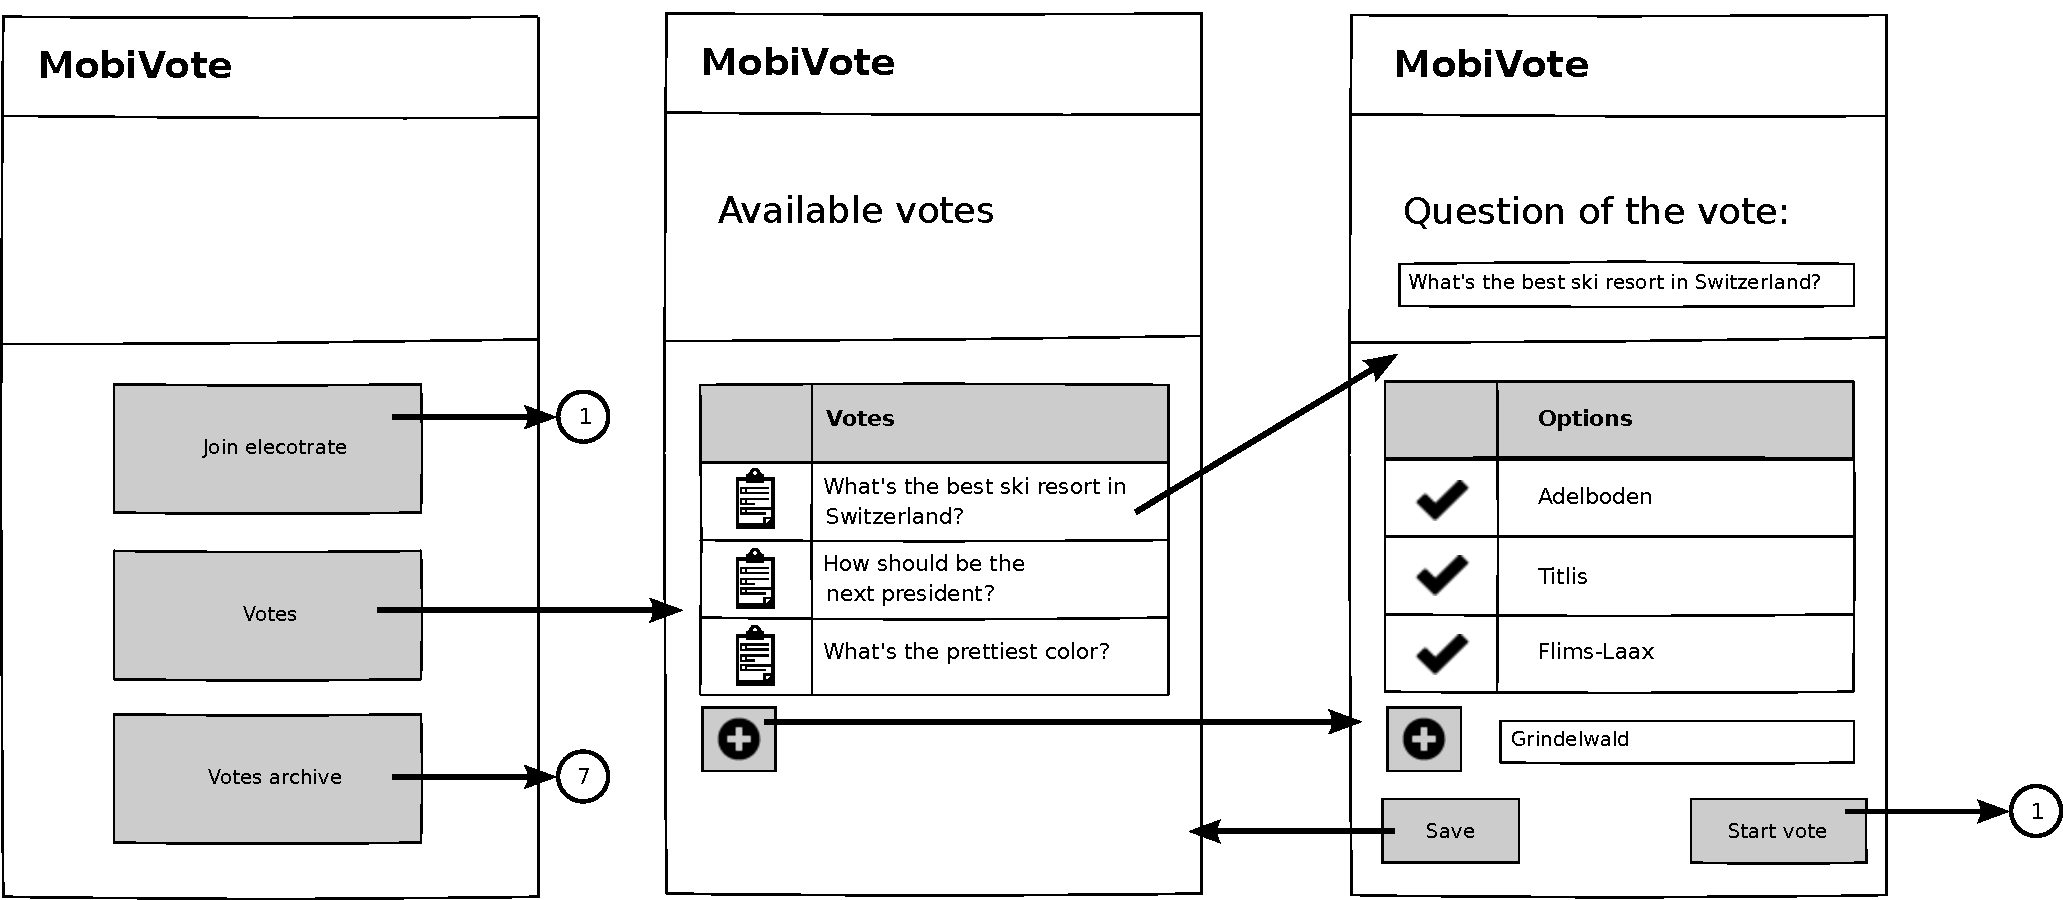
\includegraphics[height=.3\textheight]{img/storyboard/vote_setup}
	\caption{Setup a vote}
	\label{fig:vote_setup}
\end{figure}

\paragraph{Network Setup.}
The next step after defining a vote is to define in which network environment
the voting session will take place. The first person to do so is the vote
administrator. He can choose a Wi-Fi network in which the network session will
be started. The information about the chosen network as well as the generated
session password has to be shared with the participants. To do so, the
administrator can either just read the information out loud, or share the
information using either a QR-code or write the information to a NFC token which
can be passed to all participants. Using this information, the participants can
join the network session with their devices. Before joining the session, each
participant (including the administrator) has to define an identification string
for themselves. The screen design of this phase is illustrated in
\Vref{fig:network_setup}.

\begin{figure}[htb]
	\centering
	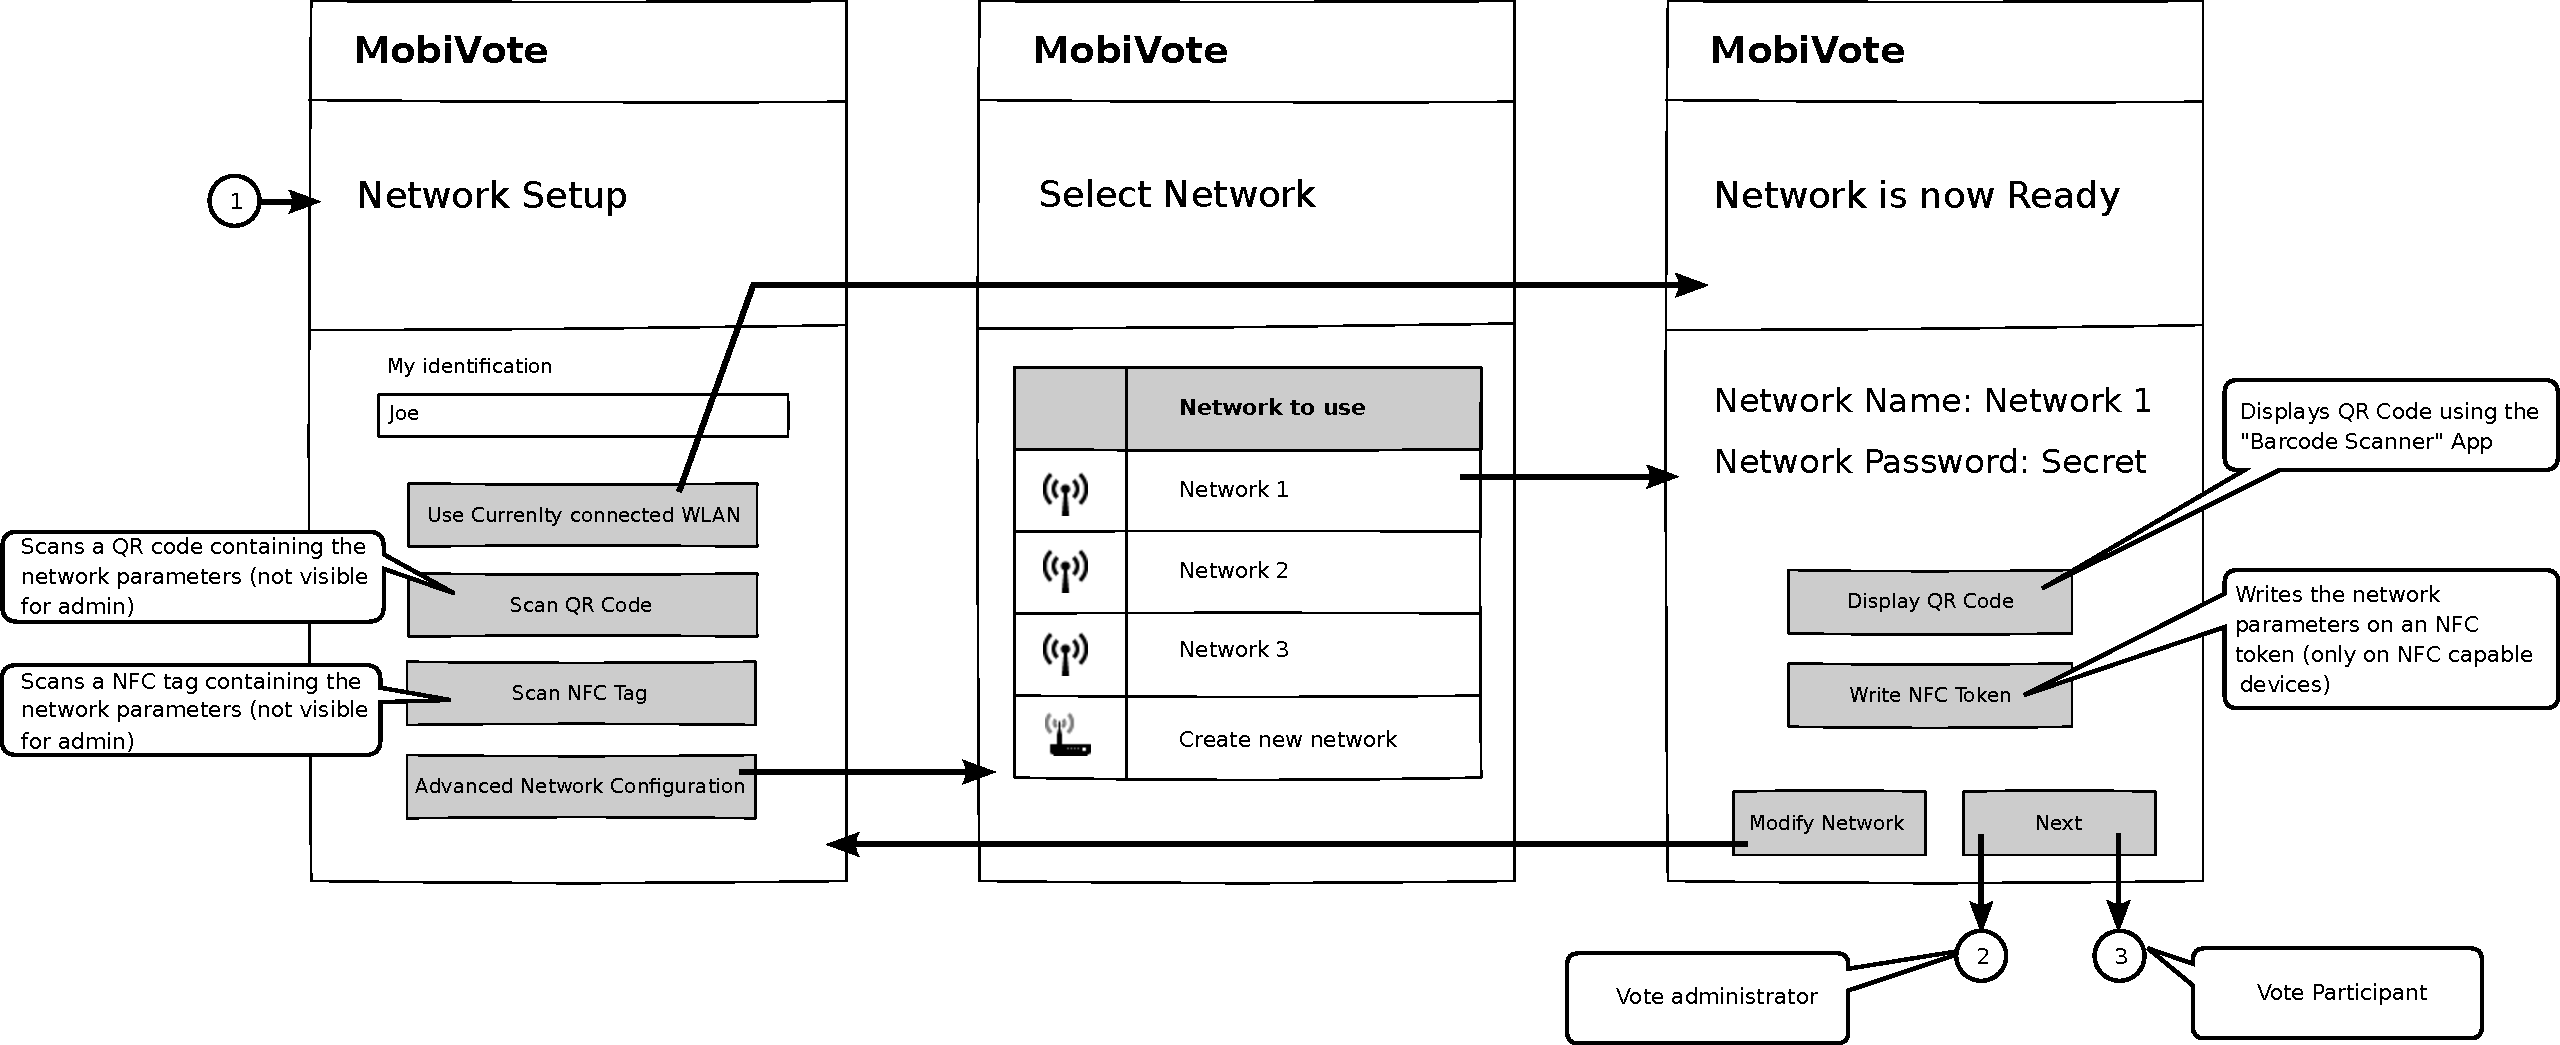
\includegraphics[height=.3\textheight]{img/storyboard/network_setup}
	\caption{Network setup}
	\label{fig:network_setup}
\end{figure}


\paragraph{Defining the Electorate and Review of the Vote.}
After joining the network session, a list of all the session participants is
displayed. At this stage, the administrator can define the electorate, meaning
he can select the participants which are allowed to vote. This can be done by
clicking on the checkboxes next to the participant's identification. The
participants can see who has been selected on their devices.

Once the administrator has defined the electorate, each participant has to
confirm that all the parameters of the vote (question, allowed options
and electorate) are correct. The vote can only be started by the administrator
if the whole electorate has agreed. If necessary, the administrator can go back and do changes on the vote parameters.

The screen design of this phase from the administrator's perspective is
illustrated in \Vref{fig:admin_review} and from the voter's perspective in
\Vref{fig:voter_review}.

\begin{figure}[htb]
	\centering
	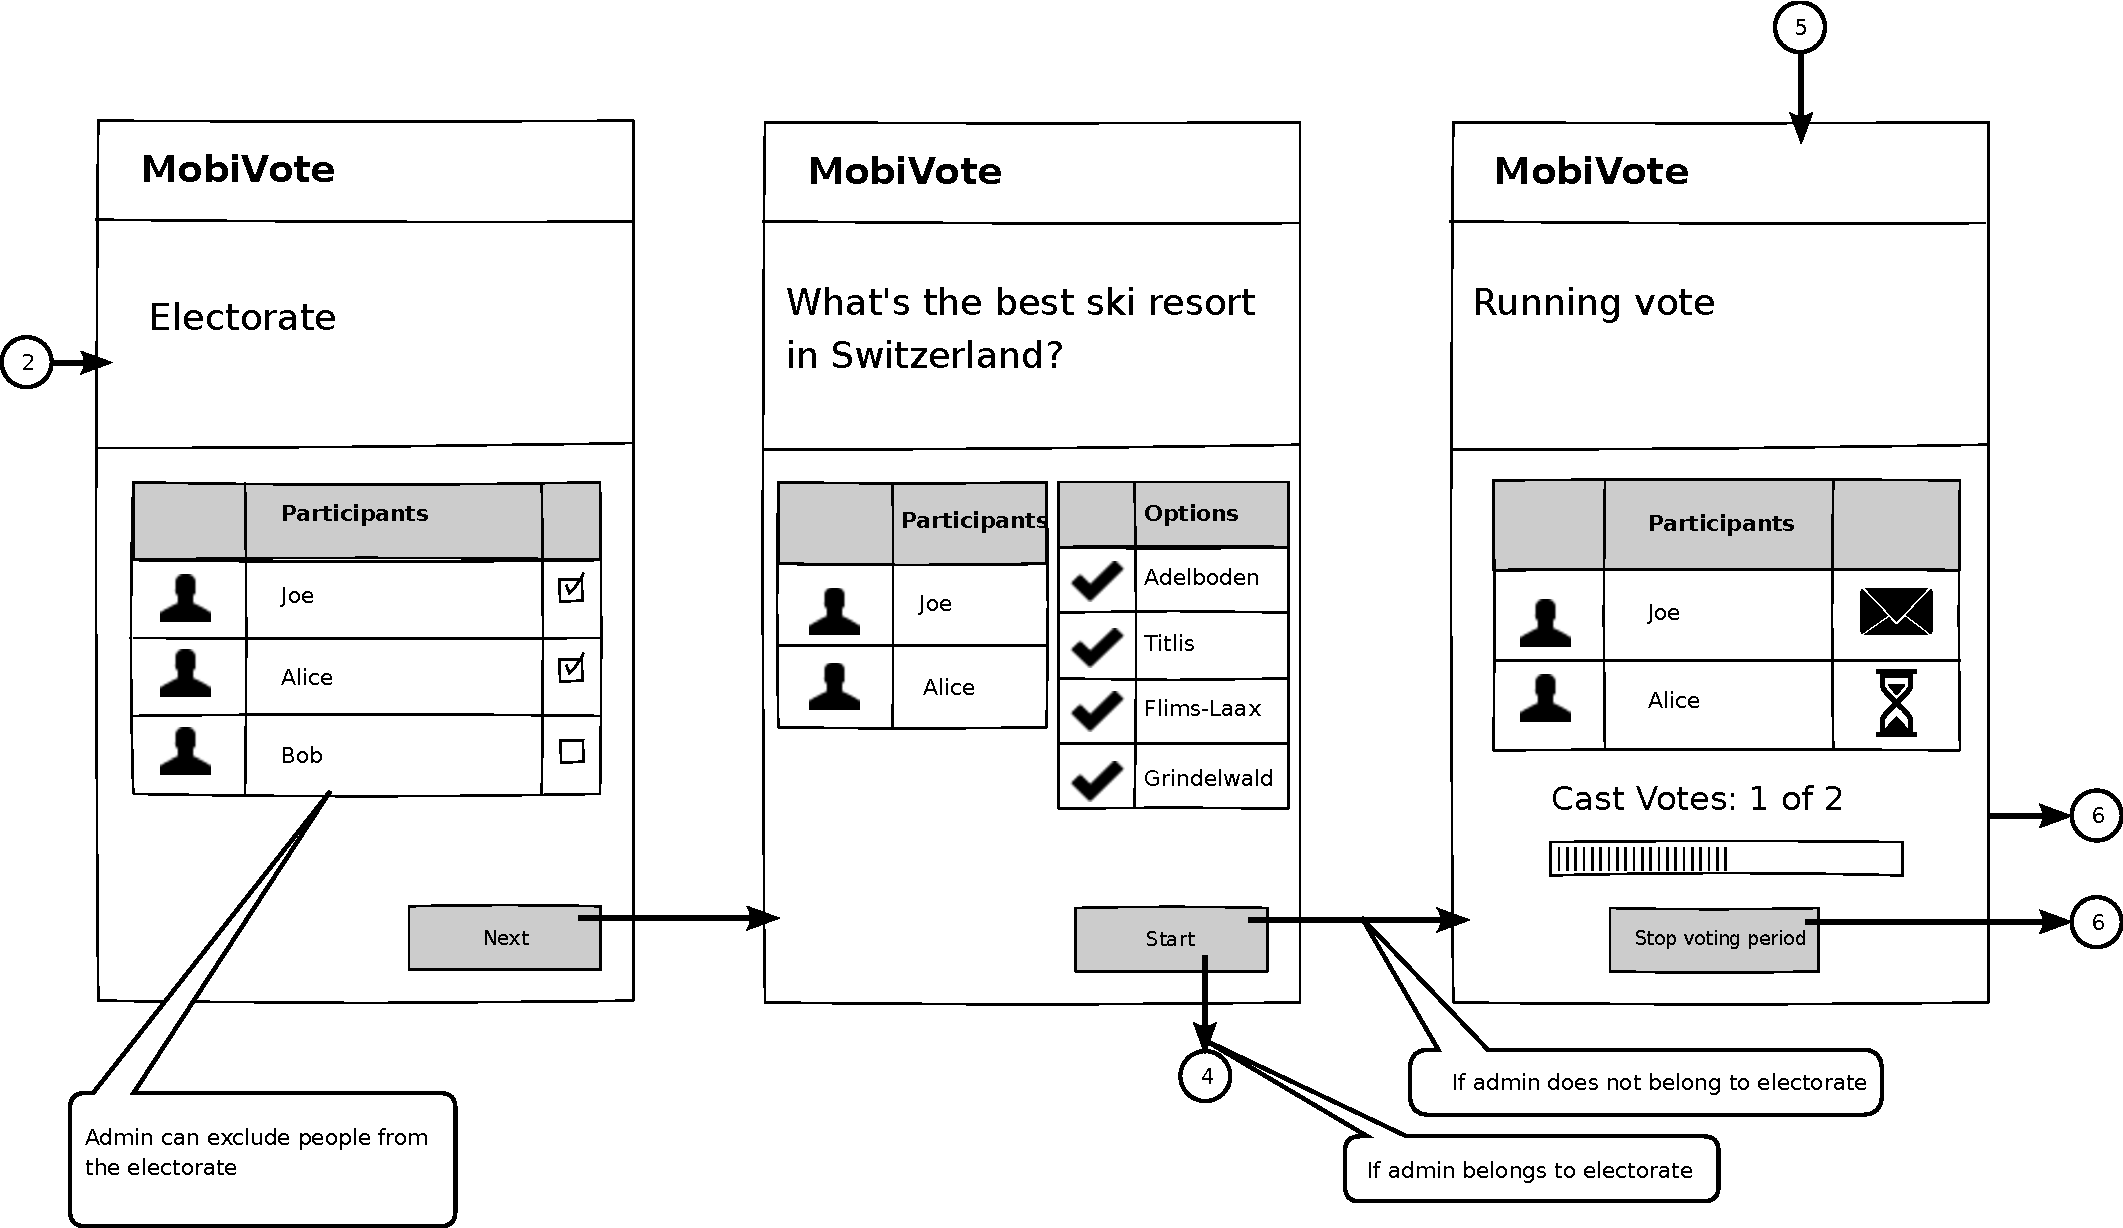
\includegraphics[height=.3\textheight]{img/storyboard/admin_review}
	\caption{Administrator defining the electorate}
	\label{fig:admin_review}
\end{figure}

\begin{figure}[htb]
	\centering
	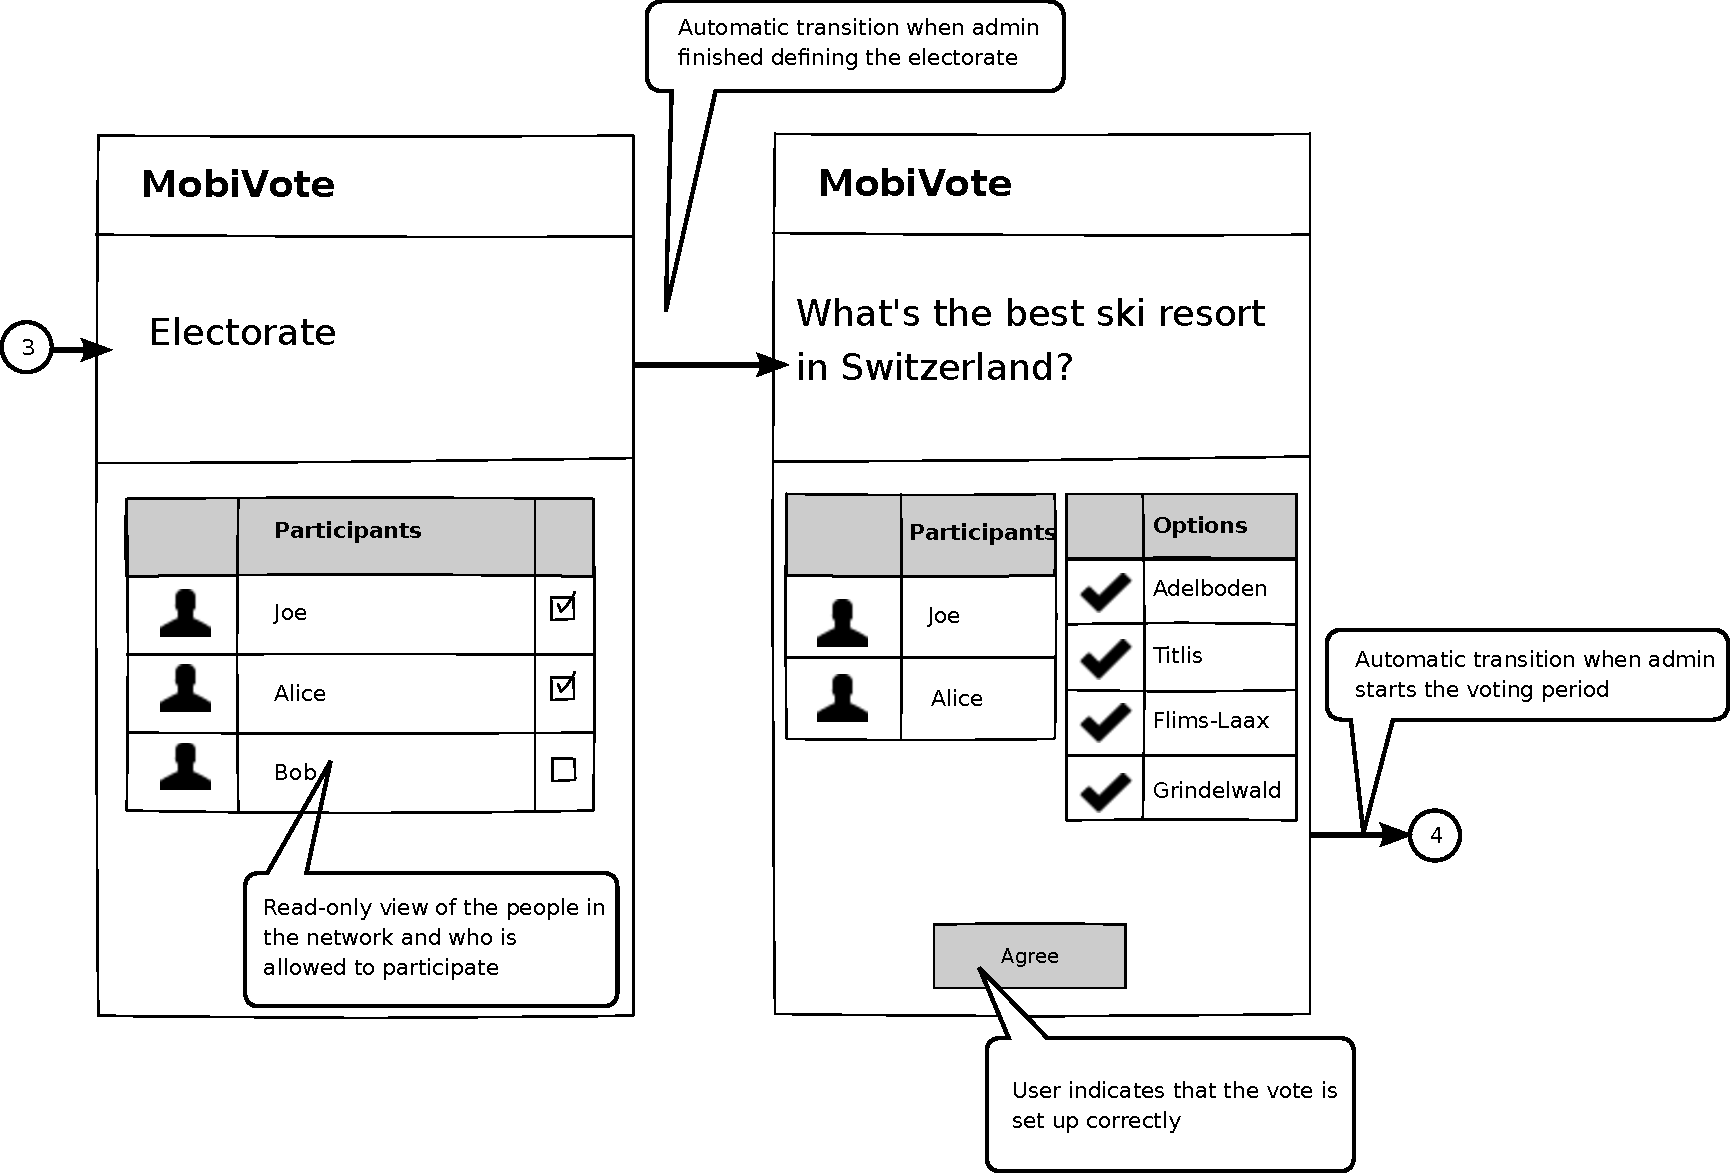
\includegraphics[height=.3\textheight]{img/storyboard/voter_review}
	\caption{Review of the vote from voter's perspective}
	\label{fig:voter_review}
\end{figure}

\paragraph{Voting phase.}
Once the vote has passed the review, the vote itself can take place. Each
participant can choose an option and cast it. The screen transitions to a view
which shows the vote casting state of all the participants. The screen
design of this phase is illustrated in \Vref{fig:vote}.

\begin{figure}[htb]
	\centering
	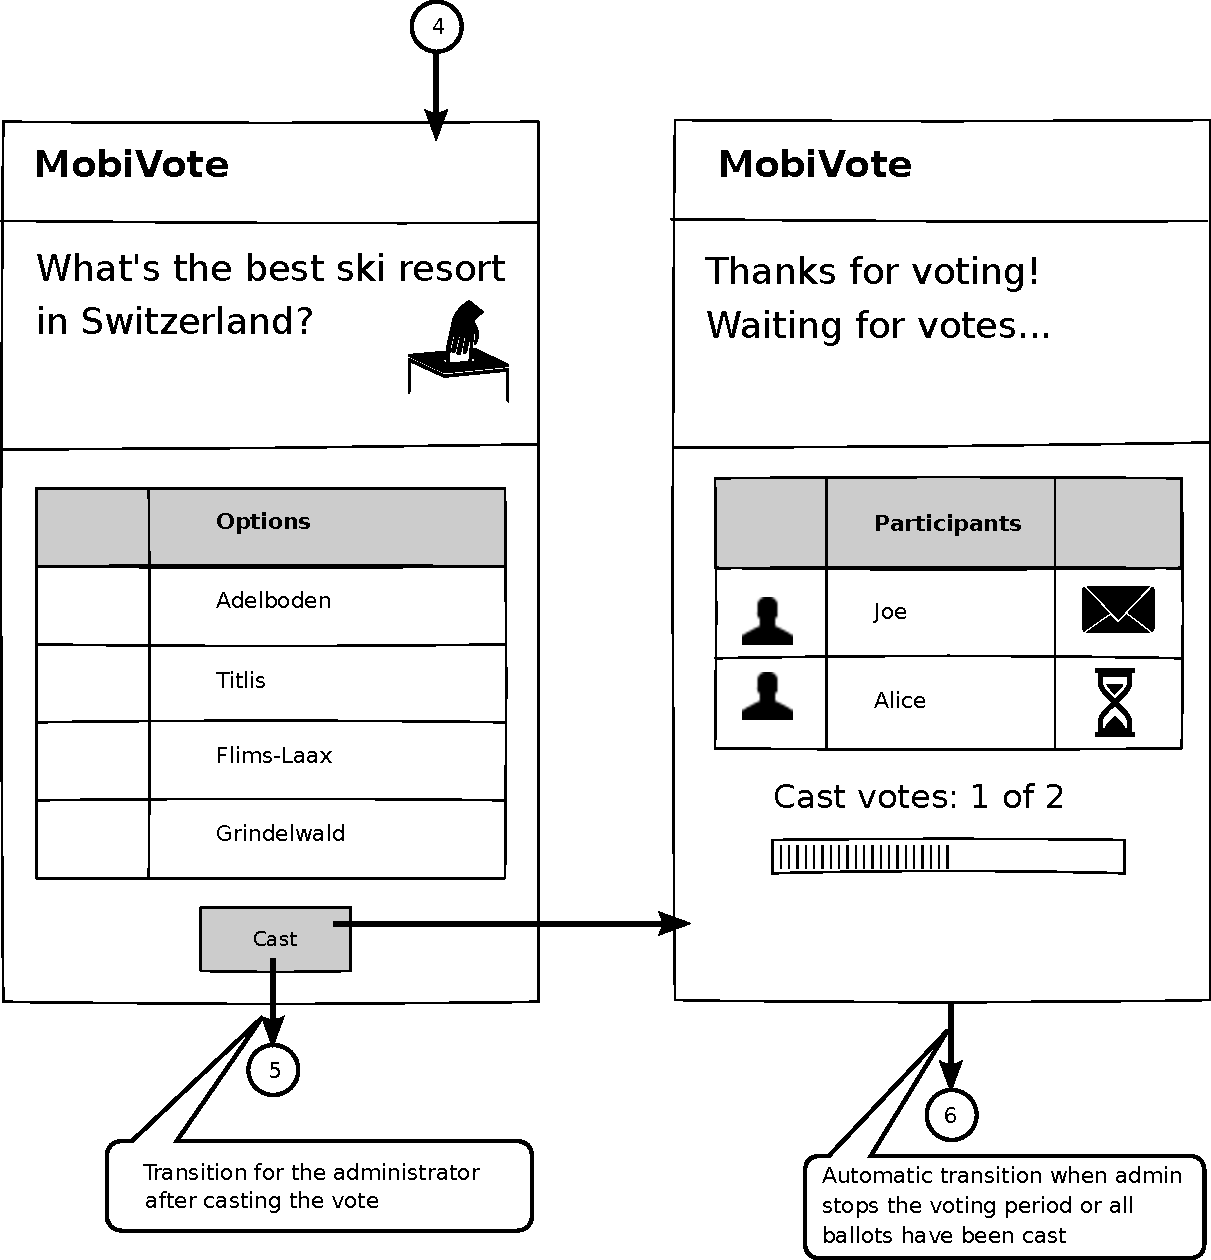
\includegraphics[height=.3\textheight]{img/storyboard/vote}
	\caption{Vote casting}
	\label{fig:vote}
\end{figure}

\paragraph{Displaying the result.}
The vote is tallied as soon as the last vote has been cast, or if the
administrator has ended the voting phase. The result is displayed in form of
a pie-chart and a tabular view. The result of the vote is saved on each device
and can be revisited using the archive function in the main screen. The screen
design of this phase is illustrated in \Vref{fig:result}.

\begin{figure}[htb]
	\centering
	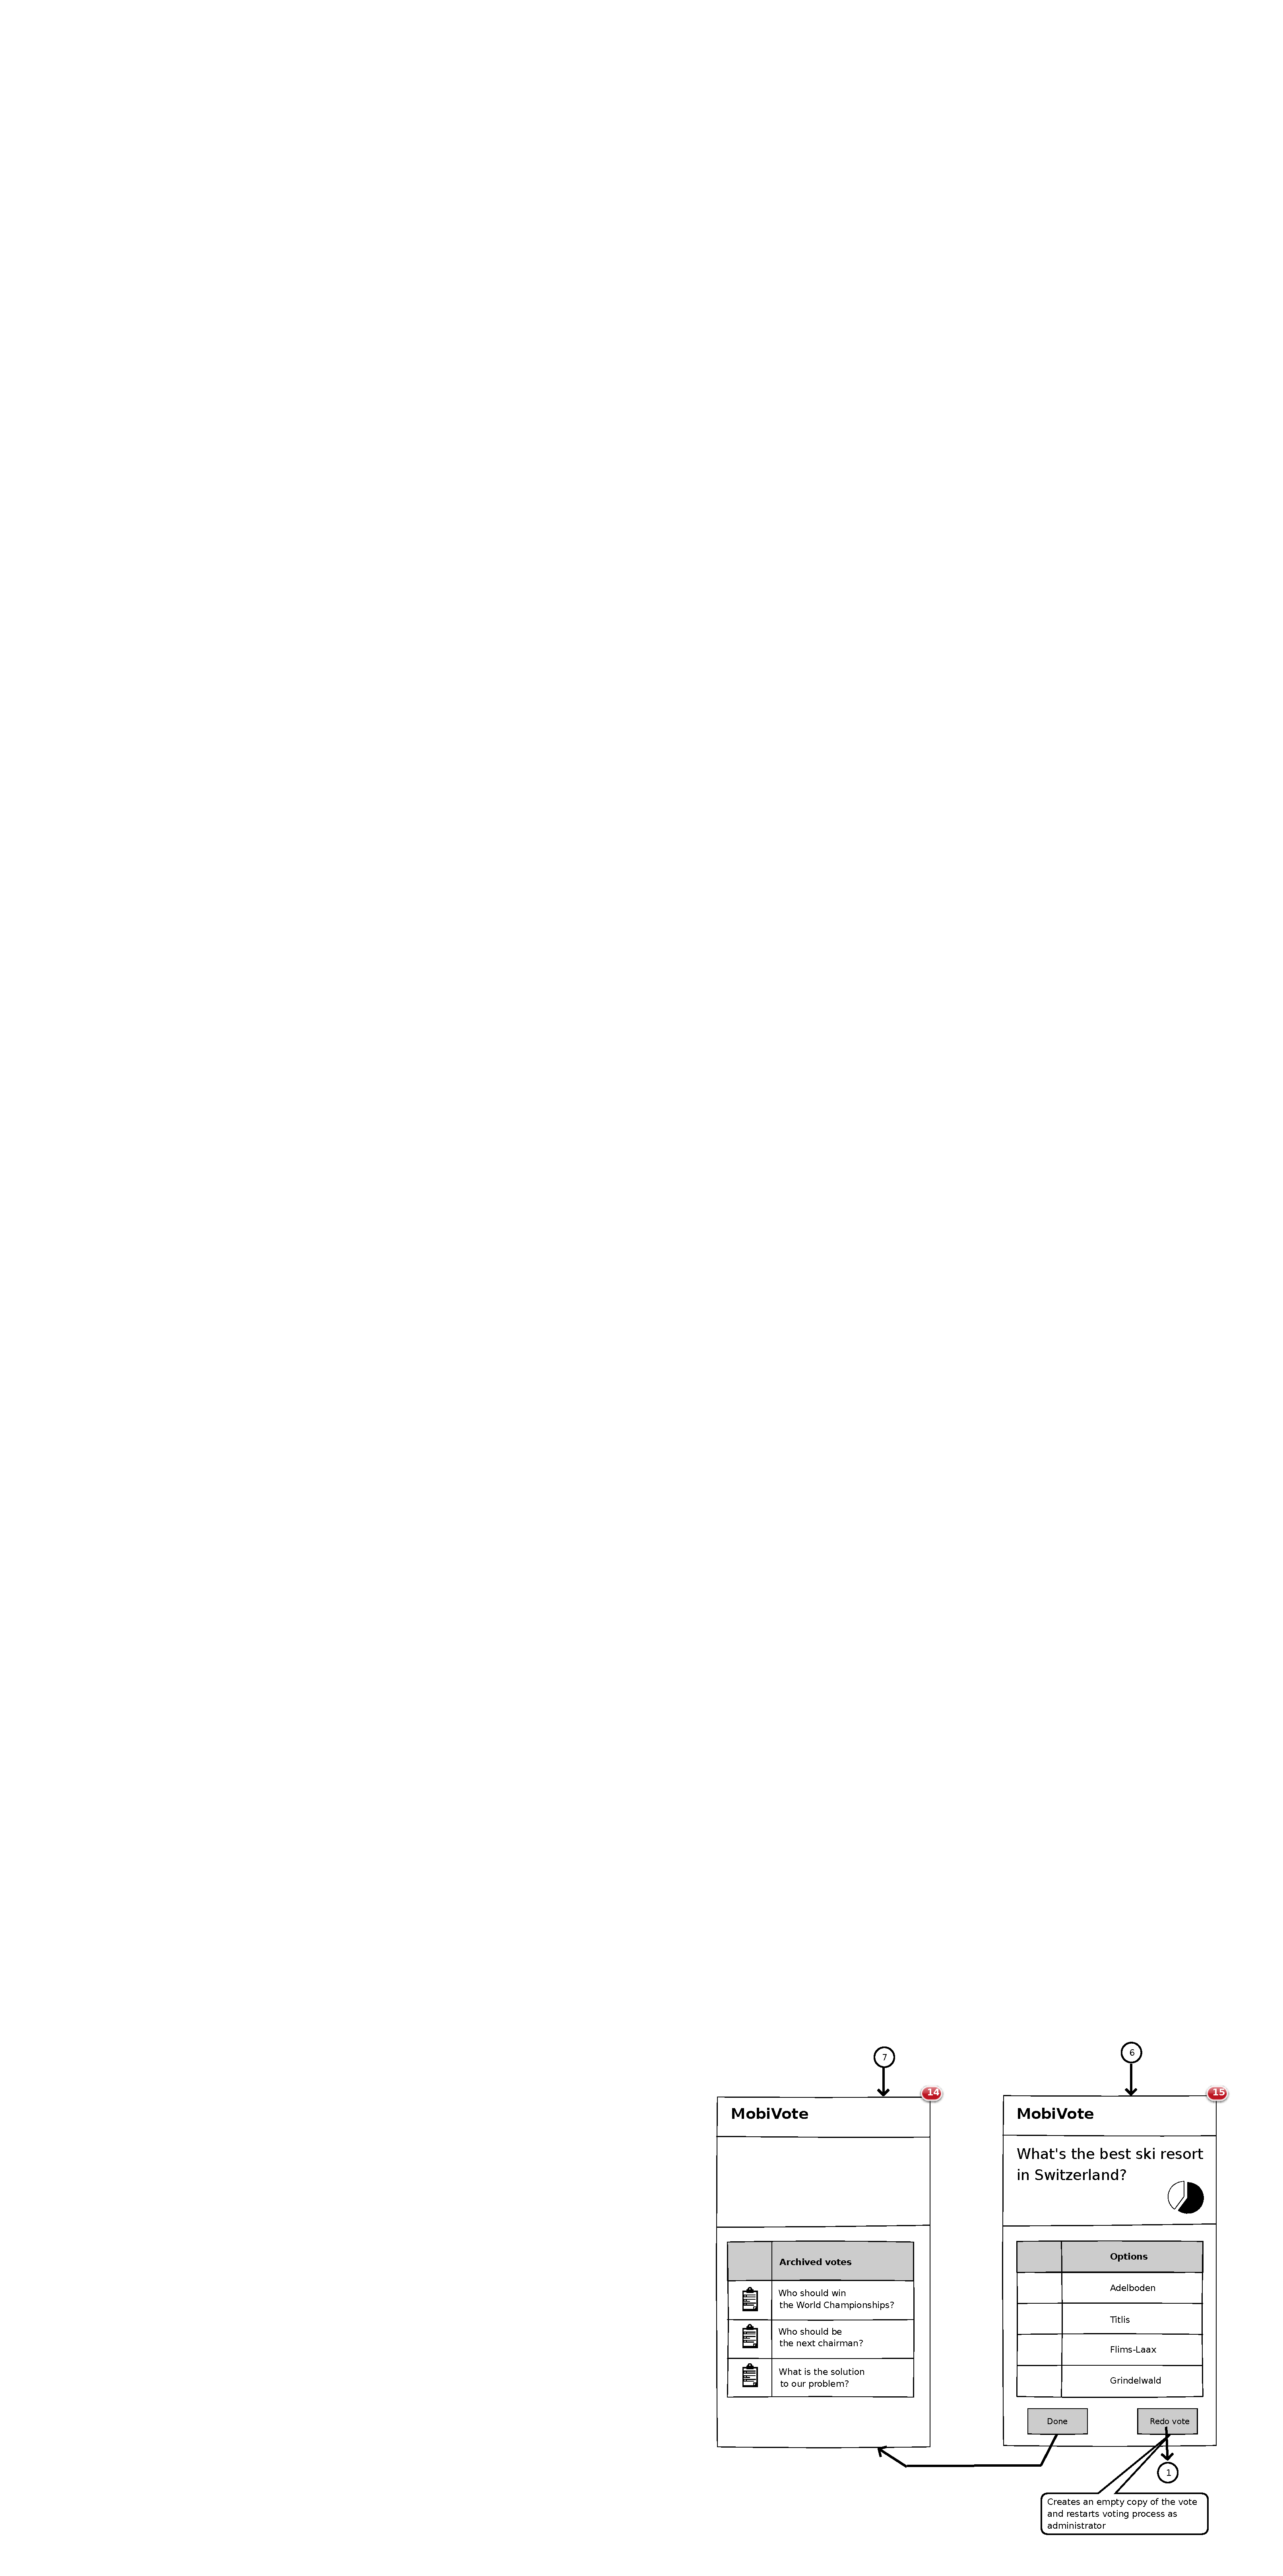
\includegraphics[height=.3\textheight]{img/storyboard/result}
	\caption{Result of the vote}
	\label{fig:result}
\end{figure}


\subsection{Implementation}
The user interface has been implemented according to the storyboard presented in
the previous section. The Android platform provides a powerful framework to
implement rich user interfaces. The framework also allows to handle different
layouts for each individual form factor. This is necessary because devices can
have different screen sizes and are normally used in different orientations. A
layout designed for a smartphone in portrait mode usually does not fit well on a
tablet in landscape mode. To deal with this issue, multiple layouts have been
developed to cope with this issue. The Android framework then automatically
applies the correct layout.



% \section{Graphical User Interface}
% \label{sec:graphicaluserinterface}
% 
% The Android platform provides a powerful framework which allows to design rich
% user interfaces specifically designed for mobile devices. The User interface was
% built using these techniques:
% 
% \paragraph{Activities.}
% Android Activities basically represent screens which allow the user to interact
% with the application. An activity is represented as a Java class inheriting from
% the Activity class. For each Activity there is a XML file which represents the
% structure of the screen layout and which elements (buttons, icons, labels,
% textfields, etc.) it contains. \Vref{tab:activities} outlines the activities and
% the corresponding layouts which have been implemented for this application.
% 
% \begin{table}[htbp]
% 	\centering
% 	\renewcommand{\arraystretch}{1.4}
% 	\begin{tabularx}{\textwidth}{llX}
% 		\toprule
% 		\textbf{Activity}			& \textbf{Layout}										\\
% 		\midrule
% 		CheckElectorateActivity 	& \texttt{activity\_check\_electorate.xml} 				\\
% 		CreateNetworkActivity		& \texttt{activity\_create\_network.xml}				\\
% 		DisplayResultActivity		& \texttt{activity\_display\_result.xml}				\\
% 		ElectorateActivity			& \texttt{activity\_electorate.xml}						\\
% 		ListTerminatedPollsActivity	& \texttt{activity\_list\_terminated\_polls.xml}		\\
% 		MainActivity				& \texttt{activity\_main.xml}							\\
% 		NetworkConfigActivity		& \texttt{activity\_network\_config.xml}				\\
% 		NetworkInformationActivity	& \texttt{activity\_network\_information.xml}			\\
% 		PollActivity				& \texttt{activity\_poll.xml}							\\
% 		PollDetailActivity			& \texttt{activity\_poll\_detail.xml}					\\
% 		ReviewPollAdminActivity		& \texttt{activity\_review\_poll.xml}					\\
% 		ReviewPollVoterActivity		& \texttt{activity\_review\_poll\_voter.xml}			\\
% 		VoteActivity				& \texttt{activity\_vote.xml}							\\
% 		WaitForVotesAdminActivity	& \texttt{activity\_admin\_wait\_for\_votes.xml}		\\
% 		WaitForVotesVoterActivity	& \texttt{activity\_wait\_for\_votes.xml}				\\
% 		
% 		\bottomrule
% 	\end{tabularx}
% 	\renewcommand{\arraystretch}{1}
% 	\caption{Activities}
% 	\label{tab:activities}
% \end{table}
% 
% 
% \paragraph{Fragments.}
% Fragments allow to reuse parts of a screen design in multiple activities. They
% are also used to design complex dialog interfaces. Fragments are always embedded
% into an activity or a dialog. Similar to activities,
% fragments also have a corresponding layout which is stored
% in a XML file. \Vref{tab:fragments} outlines the fragments and the corresponding
% layouts which have been implemented for this application.
% 
% \begin{table}[htbp]
% 	\centering
% 	\renewcommand{\arraystretch}{1.4}
% 	\begin{minipage}{\linewidth}
% 	\begin{tabularx}{\textwidth}{llX}
% 		\toprule
% 		\textbf{Fragment}						& \textbf{Layout}								\\
% 		\midrule
% 		ConnectNetworkDialogFragment			& \texttt{dialog\_join\_network.xml}			\\
% 		HelpDialogFragment						& \texttt{dialog\_help.xml}						\\
% 		IdentificationWlanKeyDialogFragment		& \texttt{dialog\_identification\_wlankey.xml}	\\
% 		NetworkDialogFragment					& \texttt{dialog\_network\_information.xml}		\\
% 		NetworkInformationFragment				& \texttt{fragment\_network\_information.xml}	\\
% 		NetworkListFragment						& \texttt{list\_item\_network.xml}\footnote{In
% 		\emph{ListFragments} the layout for each row is applied} 								\\
% 		NetworkOptionsFragment					& \texttt{fragment\_network\_options.xml}		\\
% 		NFCFragment								& \texttt{fragment\_nfc.xml}					\\
% 		PollReviewFragment						& \texttt{fragment\_poll\_review.xml}			\\
% 		ResultChartDialogFragment				& \texttt{dialog\_chart.xml}					\\
% 		ResultChartFragment						& \texttt{fragment\_result\_chart.xml}			\\
% 		WaitForVotesFragment					& \texttt{fragment\_wait\_for\_votes.xml}		\\
% 		\bottomrule
% 	\end{tabularx}
% 	\end{minipage}
% 	\renewcommand{\arraystretch}{1}
% 	\caption{Fragments}
% 	\label{tab:fragments}
% \end{table}
% 
% \paragraph{Listviews and Adapters.}
% In the Android framework, adapters are used to bind data to a layout
% representing one line in the list. These populated layouts are then displayed in
% a scrollable list. 
% \\

\section{Voting Protocol}
\label{sec:votingprotocol}
A major goal of this project is to create a decentralized e-voting system which
provides as many security properties as possible. These
properties are discussed in \Vref{sec:evoting}. The CGS97 voting scheme
\cite{CGS97} offers most of these properties. The properties of the CGS97 scheme
are discussed in \Vref{sec:CGS97}. This scheme has not specifically been
designed for decentralized e-voting systems. The protocol itself remains exactly
the same, but the assignment of some roles are slightly changed:

\paragraph{Trustees:} The CGS97 scheme stipulates the role of trustees. Trustees
are responsible to jointly generate an asymmetric key pair for the voting
session and jointly decrypt the result after the voting period has come to an end. In the
decentralized scenario, we merge the role of the trustee with the role of the
participant. This doesn't create a conflict because a trustee can also be a
participant in the vote. The fact that we assign the role of a trustee to each
participant also reduces the complexity from a usability perspective, because no
explicit assignment is required during the setup process of the vote.

\paragraph{Bulletin Board:} In classic e-voting scenarios, a bulletin board is
considered as a centralized high available infrastructure. This paradigm can't
be applied to the decentralized voting scenario because no central
infrastructure should be required. Instead, each participants creates it's own
transcript of the voting protocol. Almost all messages are exchanged by
broadcasting them to all participants of the group and can be intercepted and
recorded by each participant. In case of a manipulation, the participants would
discover the manipulation by comparing the recorded values using their physical
proximity.

\todo{Vote encoding}

\section{Bootstrapping of Group Communication}
\label{sec:bootstraping}
In order to assure privacy and authenticity of a voting session, the
communication between the participant's devices needs to be secured using
cryptographic means. To achieve that, different types of cryptographic keys need
to be exchanged. When joining a voting session, the user needs to provide a
conversation password which has been generated on the device of the vote
administrator. The administrator has several possibilities to distribute this
password, along with the other information which is needed to connect, namely
the SSID of the WLAN on which the conversation takes place and the group name to
identify the conversation. The following possibilities are available:
\begin{itemize}
  \item Communicate the password, the groupname and the SSID as text.
  Participants who want to join the session need to enter these parameters using
  the soft keyboard of the mobile device.
  \item Display a QR-code which encodes password, groupname and SSID.
  Participants who want to join the session can snap a picture of this QR-code
  using the camera of the mobile device and decode the information on their
  devices.
  \item Write password, groupname and SSID to a NFC tag which then can be passed
  along to all the participants. When tapping this NFC tag on the back of a NFC
  capable device, the User will be connected to the session.
\end{itemize}

The applications uses the password to derive an AES key which will be used to
symmetrically encrypt all the broadcast traffic in the conversation.
Furthermore, a dynamic salt which is generated by the administrator decreases
the risk of rainbowtable attacks.

In order to guarantee the authenticity and integrity of the messages in the
conversation, each participant generates an RSA key pair. The public key is 
broadcast to all the participants. This key setup can then be used for
signing/verifying all the messages in the conversation, as well as for
establishing a secure point-to-point channel between two participants in the
conversation.

For the unicast functionality of the messaging layer, a hybrid encryption
mechanism is used. To achieve this, we encrypt an AES key which is used
previously to encrypt the unicast payload using the RSA public key of the
recipient. The recipient can then use it's private key to decrypt the AES key,
and then in a second step use this AES key to decrypt the payload.

\section{Messaging}
\label{sec:messaging}
For the communication between devices and components, a messaging infrastructure
is required. We can divide the messages which are exchanged during a voting
period into two categories:
\begin{itemize}
  \item \textbf{Network Messages:} Messages which are exchanged
  between the participant's mobile devices.
  \item \textbf{Local Broadcast Messages:} This type of messages are Messages
  which are passed between Android components, for example when a user interface
  component needs to be updated if a specific event occurs. 
\end{itemize}
In order to distinguish the messages in order to decide how they should be
processed, messages types were defined. The following two sections describe the
message types which have been defined for each category and gives further
technical insight how the messaging infrastructure has been designed.

\subsection{Network Messages}
Network Messages are required to exchange messages between the mobile devices of
the participants. This is necessary for establishing the voting session, as well
as for exchanging protocol specific values, for example an encrypted ballot.
These messages are passed through a stack of communication layers.
\Vref{fig:messagingarchitecture} depicts how this stack is built. For
establishing a group communication among network devices, the AllJoyn library is
used. For the specific use in MobiVote, a wrapper library has been implemented.
The availability of this interface allows to interchange the messaging library
which is used for MobiVote. The AllJoyn Interface Library allows to send
broadcast messages, meaning the messages reach all the participant in the group.
Most of the communication is done in this manner. It is also possible to send a
message to a specific member of the group. This method is called unicast. In
order to distinguish the different purpose of the messages interchanged between
the participant's devices, a number of message types have been defined. These
message types are outlined in \Vref{tab:networkmessagetypes}.

 \begin{figure}[htbp]
	\centering
	\tikzumlset{fill component=lightgray!20}
	\tikzumlset{fill note=white} 
	\begin{tikzpicture} 
		\draw[rounded corners=0.2cm,dashed] (-3,6.8) rectangle (3,14);
		\draw (0,13.7) node {implemented during this project};
		\umlbasiccomponent[x=0, y=12, width=4cm]{MobiVote} 
		\umlbasiccomponent[x=0, y=8, width=4cm]{AllJoyn Interface Library} 
		\umlbasiccomponent[x=0, y=4, width=4cm]{AllJoyn}
		\umlbasiccomponent[x=0, y=0, width=4cm]{Android Network Stack} 
		\umlassemblyconnector[interface={\space}, anchor1=south,
		anchor2=north, name=1]{MobiVote}{AllJoyn Interface Library}
		\umlassemblyconnector[interface={\space}, anchor1=south,
		anchor2=north, name=2]{AllJoyn Interface Library}{AllJoyn}
		\umlassemblyconnector[interface={\space}, anchor1=south,
		anchor2=north, name=3]{AllJoyn}{Android Network Stack}
		
		\umlnote[x=6, y=10.2, width=5cm]{1-interface}{The AllJoyn interface library
		provides an interface to the messaging infrastructure which can be used by
		MobiVote.}
		\umlnote[x=6, y=6.2, width=5cm]{2-interface}{AllJoyn provides an API which
		allows to use the library's functionality.}
		\umlnote[x=6, y=2.2, width=5cm]{3-interface}{AllJoyn uses the network API
		provided by the Android platform.}
		
	\end{tikzpicture}
	\caption{Messaging Architecture}
	\label{fig:messagingarchitecture}
\end{figure}

\subsection{Local Broadcast Messages}
The Android framework provides an internal messaging infrastructure which allows
android component to communicate among each other. Any component can broadcast
messages using this infrastructure. These messages can be received by any
component which registered a so called Broadcast Receiver. All the registered
components will then be notified as soon as a message has been broadcast. This
mechanism can be used for example to update the User Interface according to a
specific event.
This paradigm was used heavily for the implementation of this project.


\begin{table}[htbp]
	\centering
	\renewcommand{\arraystretch}{1.4}
	\begin{minipage}{\linewidth}
	\begin{tabularx}{\textwidth}{lX}
		\toprule
		\textbf{Message Type}					& 	\textbf{Description}			\\
		\midrule
		VOTE\_MESSAGE\_ELECTORATE					& 	Used during the setup phase to
														indicate which participants are allowed to vote.\\
		VOTE\_MESSAGE\_POLL\_TO\_REVIEW				& 	Used to signal the participants that a
														vote is available for review.\\
		VOTE\_MESSAGE\_ACCEPT\_REVIEW				& 	Used by the participants to signal that
														they agree with the proposed vote.\\
		VOTE\_MESSAGE\_START\_POLL					& 	Used to signal the start of a voting
														period. \\
		VOTE\_MESSAGE\_COEFFICIENT\_COMMITMENT		& 	Used during the key generation
														phase for commiting to the chosen coefficients.\\
		VOTE\_MESSAGE\_KEY\_SHARE					& 	Used to transmit the key shares between
														participants.\\
		VOTE\_MESSAGE\_KEY\_SHARE\_COMMITMENT		& 	Used to commit to the key share
														used for performing the part decryption.\\
		VOTE\_MESSAGE\_VOTE							& 	Used to transmit a vote.	\\

		VOTE\_MESSAGE\_STOP\_POLL					& 	Used to signal the end of a voting period.\\
		VOTE\_MESSAGE\_CANCEL\_POLL					& 	Used to signal the cancellation of a
														voting period.\\
		VOTE\_MESSAGE\_PART\_DECRYPTION				& 	Used to transmit a part decryption
														after the voting period for jointly decrypting the result of the
														vote.\\
		

		\bottomrule
	\end{tabularx}
	\end{minipage}
	\renewcommand{\arraystretch}{1}
	\caption{Network Message Types}
	\label{tab:networkmessagetypes}
\end{table}

\section{Data Structures} 
\label{sec:datastructures}
In this section the used data structures to store data within the MobiVote
application are introduced.

\paragraph{Database.} For the management of the available votes in the system
(prepared as well as completed votes), a small database structure has been implemented. The Android
platform embeds the sqlite\footnote{\url{http://www.sqlite.org/}} database in
its API, hence this was the obvious choice for the database technology. \Vref{fig:erd} depicts the very simple data
structure which has been chosen for this project.

\begin{figure}[htbp]
	\centering
	\tikzumlset{fill class=lightgray!20} 
	\begin{tikzpicture} 
	\umlclass[x=0,y=0]{poll}{
		+ question : string \\
		+ starttime : int \\
		+ is\_terminated : boolean \\
		+ number\_participants : int \\
	}{} 
	\umlclass[x=8,y=0]{option}{
		+ text : string \\
		+ nbr\_votes : int \\
		+ percentage : real \\
	}{} 
	\umlassoc[geometry=--,arg1=1,align1=left, pos1=0,arg2=0..*,
	align2=left]{poll}{option}
	\end{tikzpicture}
	\caption{Entity Relationship Diagram}
	\label{fig:erd}
\end{figure}

According to the Android best practice, a \texttt{SQLiteOpenHelper} class has
been implemented which manages all the database communication. It also takes
care about the mapping between entity objects and database entries.
\Vref{fig:entities} depicts the implemented entity classes. The entity class
which represents a participant does not have a corresponding database identity,
this is because the participants of the vote is defined during the voting cycle.
It is also not relevant later on when displaying the result of the vote,
therefore the information about the participants are not stored in the database.

\begin{figure}[htbp]
	\centering
	\tikzumlset{fill class=lightgray!20} 
	\begin{tikzpicture}
	\umlclass[x=6,y=5]{Poll}{
		- id : int \\
		- question : String \\
		- options : List<Option> \\
		- participants : Map<String,Participant> \\
		- numberParticipants : int \\
		- startTime : long \\
		- isTerminated : boolean \\
	}{
		+ \emph{accessor methods}
	} 
	\umlclass[x=0,y=0]{Option}{
		- id : int \\
		- pollId : int \\
		- text : String \\
		- votes : int \\
		- pecentage : double \\
	}{
		+ \emph{accessor methods}
	} 
	\umlclass[x=11,y=0]{Participant}{
		- identification : String \\
		- uniqueId : String \\
		- hasVoted : boolean \\
		- isSelected : boolean \\
		- hasAcceptedReview : boolean \\
	}{
		+ \emph{accessor methods}
	} 
	\umlassoc[geometry=-|,arg1=1,arg2=0..*,pos1=0.1, pos2=1.9]{Poll}{Option}
	\umlassoc[geometry=-|,arg1=1,arg2=0..*,pos1=0.1, pos2=1.9]{Poll}{Participant}
	\end{tikzpicture}
	\caption{Entity Class Diagram}
	\label{fig:entities}
\end{figure}

\paragraph{XML Serialization.} In order to make a vote verifiable, all the
relevant values such as cryptographic parameters, encrypted ballots, zero-knowledge proofs, etc. of the
CGS97 voting protocol are serialized into a simple XML file. To do so, we are
using the Simple framework. Using this framework, we can create a set of classes
which are used to store all the values which should be written into a file.
Instructions how the serialization should happen are defined using annotations
in the class. This type of simple class is also known as POJO (Plain Old Java
Object)\footnote{\url{http://en.wikipedia.org/wiki/Plain_Old_Java_Object}}.
These POJO classes could later be used for writing a verifier software which
allows to check a vote by a third party software. The POJO classes can be found
in the Java package \texttt{ch.bfh.evoting.voterapp.protocol.cgs97.xml}.

\section{Testing}
\label{sec:testing}
To verify the correct behaviour of the implemented product, a number of
different tests have been conducted during the implementation phase. These
testing activities are outlined in the following.

\subsection{Functionality Tests}
\label{sec:functionalitytests}
The test of the functionality mostly took place right after the implementation
step. The functional tests were all done manually on the available devices. The
devices outlined in \Vref{tab:testinginfrastructure} were available for testing the
functionality.

\begin{table}[htbp]
	\centering
	\renewcommand{\arraystretch}{1.4}
	\begin{minipage}{\linewidth}
	\begin{tabularx}{\textwidth}{lll}
		\toprule
		\textbf{Device}	&  \textbf{Formfactor} & \textbf{Android Version} 	\\
		\midrule
		Samsung Galaxy S 3		& Smartphone	& 4.3 (Samsung original)	\\
		Samsung Galaxy S 1  	& Smartphone	& 4.3.1
		(CyanogenMod)\footnote{\url{http://www.cyanogenmod.org/}}		\\
		Samsung Galaxy Tab 10.1	& Tablet		& 4.0.4 (Samsung original)	\\
		\bottomrule
	\end{tabularx}
	\end{minipage}
	\renewcommand{\arraystretch}{1}
	\caption{Testing Infrastructure}
	\label{tab:testinginfrastructure}
\end{table}

\subsection{Usability Tests}
\label{sec:usabilitytests}
The implementation phase of this project started with the implementation of the
Graphical User Interface of the application. At this stage, it was possible
setup and run a vote on multiple devices, but without the security of the later
implemented e-voting protocol. This implementation was then used to verify that
the user interface of the application does not cause any confusion among users.
Several people were asked to use the application and provide feedback, which
then got compiled into the implementation. The implementation of the e-voting
protocol mostly took place behind the scenes, there were only some slight
modifications in the user interface necessary to add this functionality.

\subsection{Performance Tests}
\label{sec:performancetests}
In a decentralized environment, the load which each device has to handle grows
with the number of participants and the number of options in a vote. In order to
verify that the implementation is able to handle scenarios with more than just
3 participants, 17 LG Nexus 5 smartphones running Android version 4.4 were
available to test more complex scenarios. Various tests with different scenarios
have been performed and assessed regarding time consumption in the two most time
consuming steps, namely casting a ballot tallying a vote. The results of these
performance tests are shown in \Vref{tab:perftestresults}. The performance tests
were executed using the two separate ballot encoding strategies as discussed in
\Vref{sec:ballotencoding}. Another relevant factor regarding performance is the
bit lenght of the cryptographic parameters $p$ and $q$. For all tests,
parameters with the length of 2048 bits have been used.

\begin{table}[htbp]
	\centering
	\renewcommand{\arraystretch}{1.4}
	\begin{minipage}{\linewidth}
	\begin{tabularx}{\textwidth}{cccccc}
		\toprule
		& & \multicolumn{2}{c}{\textbf{Single Ballot}} &
		\multicolumn{2}{c}{\textbf{Multi Ballot}} \\
		& & \multicolumn{2}{c}{\textbf{Encryption}} &
		\multicolumn{2}{c}{\textbf{Encryption}} \\
		\textbf{Options}	&  \textbf{Participants} & \textbf{Cast Ballot} &
		\textbf{Tallying} & \textbf{Cast Ballot} &	\textbf{Tallying}
		\\
		\midrule
		4 & 3 & \SI{2.0}{\second} & \SI{1.2}{\second} & \SI{3.7}{\second} & 
		\SI{3.7}{\second} \\
		4 & 4 & \SI{2.0}{\second} & \SI{1.3}{\second} & \SI{3.4}{\second} &	
		\SI{3.6}{\second} \\
		4 & 5 & \SI{2.0}{\second} & \SI{1.3}{\second} & \SI{3.2}{\second} & 
		\SI{4.0}{\second} \\
		6 & 3 & \SI{2.6}{\second} & \SI{1.2}{\second} & \SI{4.3}{\second} &	
		\SI{4.8}{\second} \\
		6 & 4 & \SI{2.4}{\second} & \SI{1.5}{\second} & \SI{4.8}{\second} &	
		\SI{5.4}{\second} \\
		6 & 17 & \SI{2.5}{\second} & \SI{39.0}{\second} & \SI{4.6}{\second} & 
		\SI{22.0}{\second} \\
		10 & 17 &  &  & \SI{6.7}{\second} &	
		\SI{47.2}{\second} \\
		\bottomrule
	\end{tabularx}
	\end{minipage}
	\renewcommand{\arraystretch}{1}
	\caption{Performance Test Results}
	\label{tab:perftestresults}
\end{table}

These results clearly show that the single encryption ballot strategy is the
better choice for small voting scenarios, looses its advantages in bigger
scenarios because the number of combinations which have to be checked during the
tallying process grows factorially. One combination check (which is
baiscally a modular exponentiation) was measured to take around
1.8 milliseconds on a LG Nexus 5 smartphone. In the scenario with 10 options and
17 participants, the tallying process would take roughly 2 hours and 40 minutes.
Using the multi encryption ballot strategy on the other hand, tallying the same
scenario takes 42 seconds. 

The performance tests were executed on modern smartphone hardware which can
perform expensive operations such as generating encryptions and proofs in a
reasonable time. The user experience on older devices such as the Samsung Galaxy
S1 offer a less smooth user experience, especially when using the multi
encryption ballot strategy which requires much more calculation power for
creating and verifying ballots.

\section{UniCrypt Extensions}
\label{sec:enhancmentsunicrypt}
The CGS97 protocol contains a few building blocks which were not part of the
UniCrypt library by the time this project started. Part of the goals of this
project was to enhance UniCrypt so that the logic could be used in the
implementation of this application and make it also reusable in further upcoming
projects. In the following we describe how this implementation has been done.

\subsection{Shamir Secret Sharing Scheme}
In 1979, A. Shamir proposed a scheme \cite{Shamir79} on how a secret can be
split into several independent pieces which can be distributed among several
authorities. It is not possible to recover the secret unless a sufficient amount
of these authorities collaborate in order to recover the secret. Further details
regarding this scheme can be found in \Vref{sec:secretsharing}.

\paragraph{Implementation.} The implementation has been embedded into the
existing UniCrypt structure.
The class in which the implementation has been done is the following:

\texttt{ch.bfh.unicrypt.crypto.schemes.sharing.classes.ShamirSecretSharingScheme}
\\
\\
The instantiation of this scheme requires three parameters:
\begin{itemize}
  \item An algebraic field of the type \\
  \texttt{ch.bfh.unicrypt.math.algebra.dualistic.classes.ZModPrime}. The secret
  which should be shared later on has to be an element of this field.
  \item The number of shares which should be produced
  \item A threshold value which defines how many shares must be reunited in
  order to recover the secret
\end{itemize}

A secret can be shared using the method \texttt{share()}, which takes
a message as an argument. The message must be an element of the field which has
been specified during the initialization of the scheme. The method returns an
array of value pairs. Each pair represents a share.

The secret can be recovered using the method \texttt{recover()}, which takes an
array of value pairs as an argument. The array must at least contain as many
value pairs as specified with the threshold value during instantiation. The
method returns a single element which represents the recovered secret.

\paragraph{Testing.}
UniCrypt components are tested using the JUnit\footnote{\url{http://junit.org/}}
framework. A JUnit Test for the Shamir Secret Sharing scheme has been implemented in order to check the correct
functionality after each change that is done in the UniCrypt library. The
following testclass has been implemented:

\texttt{ch.bfh.unicrypt.crypto.schemes.sharing.ShamirSecretSharingSchemeTest}

\subsection{ElGamal Proof of Validity}
A proof of validity is required if a party wants to prove that an ElGamal
ciphertext is the encryption of element of a set of possible plaintexts without
revealing which one it is. \Vref{sec:proofofvalidity} covers this topic in
further detail.

The implementation of the this proof has been done in a very early stage of this
project, according to the architecture of UniCrypt 1. In the meantime, UniCrypt
has been completely reengineered. The validity proof has been reimplemented
independently of this project in order to fit into the new architecture. Since
this project is based on UniCrypt 2, the project makes use of the reimplemented
version of the ElGamal proof of validity.


\chapter{Discussion}
\label{cha:discussion}
At the end of this project, we reached the goal of creating an e-voting
application which runs on mobile devices and can be used without additional
infrastructure and offers security features such as privacy, anonymity and
verifiability. This chapter reflects on certain aspects of this work.

\section{Decentralized E-Voting}
\label{sec:discussiondecentralizedevoting}
This section reflects the term \emph{decentralized} in relation to this project
and what approaches have been chosen to achieve this property.

\paragraph{Communication Layer:} During this project we implemented an e-voting
system which does not require any other infrastructure than the devices of the
participants (smartphone or tablets). As a communication layer for the
communication between the devices, WLAN is used. Many facilities provied a WLAN
infrastructure. The application provides the functionality to use this
infrastructure, but also offers the possibility to set up a new WLAN network
using the hot spot functionality of Android. The hot spot integrated in older
devices are usually not as powerful as a hotspot which is designed for large
networks. For larger scenarios it is recommended to use a proper infrastructure
WLAN hot spot as the communication layer. One can argue that this violates the
principle of decentralization. This is true for the base communication layer,
but it does not affect the decentralized behaviour of the e-voting protocol
which is running on top of this communication layer.

\paragraph{Messaging Layer:} In a preceeding project, a decentralized messaging
infrastructure for Android called InstaCircle \cite{ritter13a} has been
implemented. The goal is to establish a group communication so that the
participating devices can exchange message among each other. The message
exchange in InstaCircle is based on broadcasts in an IP network.
Because broadcast communication does not offer a reliable message exchange, this
approach turned out to be not reliable enough in certain network situations. The
messaging layer has been replaced by the AllJoyn library \myref{sec:alljoyn}.
In contrast to InstaCircle, the initiator of a group takes the role as a master
who orchestrates the communication within the group. In some sense, this too
violates the principle of decentralization. The choice of this architecture can
be justified for two reasons though: 
\begin{itemize}
  \item The master only orchestrates the message exchange. Attempts to cheat on
  the e-voting protocol layer would be recognized by the protocol.
  \item In a voting session, some sort of administrator is necessary. This
  person is predestined to take the master of the group communication as well.
\end{itemize}
Regardless of who manages the group communication, from an infrastructure point
of view, the communication between the devices can still be done in a
decentralized manner.

\paragraph{E-Voting Protocol:} As we have seen in \Vref{sec:CGS97}, the protocol
has not specifically been designed to be used in decentralized scenarios. The
protocol has been adapted in two major points in order to achieve this property:
\begin{itemize}
  \item All the participants become trustees and contribute to the key
  generation and decryption process
  \item All participants have their own bulletin boards
\end{itemize}
More details regarding these modifications can be found in
\Vref{sec:votingprotocol}. The fact that there is no central bulletin board also
means that there is no master on which final result is derived from. Even though
several security measures have been built into the application, we still have to
consider that this software runs on devices which are potentially compromised.
For example, a malware could fake the screens when the application asks for
input or displays the result.
At this point, we can take advantage of the fact that the votes only take place
in a confined space where the participants can communicate visually and orally
without using their devices. In the case of a disagreement on the official
result of the vote, the participants can compare the result displayed on their
device and then take one of the following actions:
\begin{itemize}
  \item Agree on the result which is displayed on the majority of devices.
  \item Rerun the vote, potentially with different devices.
\end{itemize}
Using this method of negotiating without using the devices should allow to agree
on an official result of the vote.

\paragraph{Verifiability:} Using the recorded values on the bulletin board, the
whole voting cycle can be verified. It stands for itself that the MobiVote
application verifies all the values, but in order to increase the confidence in
MobiVote, it would be desirable that a vote can be verified by an external
software. To do so, MobiVote offers the functionality to export the values of
the bulletin board to an XML file, which then can be used as an input for an
external verifier software.
One missing link in this verifiability chain stems from the fact that that the
identities used in a vote are created ad-hoc when establishing the group
communication before voting. That means that the integrity of the messages which
are exchange can only be verified during the session. Of course, the public keys
of all participants used during a particular voting session could also be
exported, but could be replaced along with all the signatures which are
recalculated using the secret key corresponding to the new public key. This
missing link could be added by using identities verified by a trusted authority,
for example with digital certificates. Dealing with certificates usually has a
significant negative impact on the usability. Furthermore, only a minority of
people are in possession of such a digital certificate which could be used as a
digital identity during the voting process. 

\section{Usability}
\label{sec:discusionusability}
In retrospective, the decision to create a proper storyboard before we started
to implement the user interface was a very good decision. It forced to reflect
on how such a spontaneous e-voting process should look like in practice. It turns
out that the process in such a spontaneous manner looks different compared to a
classic e-voting scenario in many ways. For example, we need to find a way on
how the electorate and setup can be defined and, more importantly, approved
by everybody before the vote itself can start. When we consider classic voting
scenarios, the electorate is clearly defined in advance, for example all
eligible citizen of a country. The same is true for defining how the question
and the possible options should be defined. Quite some paperwork usually
preceds a vote, whereas in a spontaneous vote, the setup needs to be approved
somehow.

Before implementing the actual e-voting protocol which provides the e-voting
specific security measures, we had an implementation ready which allowed to
perform a votes in a decentralized manner, but didn't offer the desired
security. We used this stage to do tests of the communication layer and, more
importantly usability, tests \myref{sec:usabilitytests}. The fact that the user
interface at this stage and at the final stage almost look identical shows two
things:
\begin{itemize}
  \item We were able to implement the e-voting protocol in an almost transparent
  manner. 
  \item The storyboard that has been designed seems to be universal and not
  specific to this implementation.
\end{itemize}
The latter fact is also underpinned by the fact that the partner project came to
the same conclusion \myref{sec:comparisontopartnerproject}.

\section{Security Considerations}
It speaks for itself that security plays a crucial role in the context of
e-voting. In this project we employed modern cryptographic techniques which are
the answers to many threats. Nevertheless we had to make some compromises. Most
of them relate to the tradeoff between security and usability. This section
should give an overview of these compromises.

\paragraph{Public Key Exchange:} In order to guarantee the authenticity of
messages which have been exchanged during a voting session, each participant
needs a secret key for signing all the outgoing messages. All the other
participants need to be in possession of the corresponding public key, which
they use to verify incoming messages of that particular sender. Obviously these
public keys have to be exchanged at the beginning of the session. Of course,
these keys can be transmitted using the existing network communication layer,
but since these keys are not linked to a real life identity, we can only assume
that the key really belongs to the sender. During this key exchange process, a
participant could hence impersonate somebody else. The key exchange happens on
the secured layer, so that impersonation would have to be done by a participant
who is in possession of the group password. This fact reduces the risk
significantely, because since all participants are gathered in the same physical
space, the fact that something is wrong would be discovered. The fact that
non-certified keys are used for each session also makes it impossible to verify
the authenticity of the messages after the voting session.

This problem could be solved if each participant has its own certificate, which
is a certified digital identity that lasts for longer than just a voting
session. Unfortunately only a small percentage of people possess a digital
certificate nowadays. Requiring such a certificate would narrow the group of
potential users further down and would have a negative impact on the security.

\paragraph{Untrusted Devices:} Nowadays, smartphones are little computers which
allow to run all sort of software. The ever growing popularity of these devices
also caused malware to appear. Malware could be employed to circumvent security
measures, for example by showing a user a fake screen on its devices. For
example, during a vote with options A and B, the malware would display option B
instead of A and vice versa. This causes a voter that intends to vote for option
A to vote for option B. Malware could also be used to collect information on how
a participant voted. Dealing with untrusted platforms is subject of ongoing
research and is out of scope of this project. 

\section{Comparison to the Partner Project}
\label{sec:comparisontopartnerproject}
During the same period, a project with the same focus, but with a different
e-voting protocol has been implemented \cite{vonBergen14}
\myref{cha:organization}. This allows us to compare each others implementation.
In both projects, the specified e-voting protocol could be implemented
successfully. Also, both projects share the same user interface, which shows
that the storyboard is generic. There is only one small deviation in the
implementation of this project, namely the threshold parameter which has to be
defined in the secret sharing part of the CGS97 e-voting protocol. Sharing the
same user interface also means that the protocol implementation could be merged
into a single app and let the user choose which protocol to use.

As we found out, both protocols have their own advantages and disadvantages,
mainly in the area of performance. The HKRS12 protocol \cite{HKRS12} which has
been implemented in the partner project is specifically designed for this kind
of voting scenarios. It is also a very slim protocol which results in a faster
execution, especially on slower devices. A disadvantage is the fact, that the
decoding step of the HKRS12 protocol requires an exhaustive search of
combinations in order to avoid the discrete logarithm problem, very similar to
the single encryption ballot encoding used in this project
\myref{sec:singleencriptionballot}. This means that the time consumption of the
tallying process grows rapidly as the number of participants and options grow.
In this implementation we have the same problem when using the single encryption
ballot strategy, but in this implementation we have the option to switch to the
multi encryption ballot strategy \myref{sec:multiencriptionballot}.

\section{Challenges}
Along the way to the finished app, there were a few challenges to overcome. This
section should give an overview on some points that turned out to be a bit more
challenging than anticipated.

\paragraph{Decentralized communication:} The original plan was to employ the
InstaCircle communication infrastructure in the project. InstaCircle is a
completely decentralized communication infrastructure. That also means that here
is no master instance which manages the overall state of the communication
session. Problems with synchronisation and reliability arise. This is one reason
that the communication layer has been switched to the AllJoyn library.

\paragraph{Security - Usability Trade-off:} From a user's point of view,
security usually puts many obstacles in the way. PIN-codes, Passwords, Keys,
Certificates and similar things are confusing the users. To keep the usability
on an acceptable level, some compromises have been made. One such compromise is
the use of non-certified identities. Of course, the design of a usable user
interface was quite a challenge on its own.

\paragraph{Android Wifi API:} The android platform provides an API for managing
the Wireless connections on an Android device. This API is used in our
application to properly configure the network on which the voting session is
going to take place. Despite the documentation, it took quite some time to
figure out how this API can be used properly.

\paragraph{Robustness in many Situations:} An application running on a mobile
device has to be in a way that it can deal with many unexpected situations. For
example, an incoming phone call should not disrupt the entire ongoing voting
process. In a voting scenario with many participants, the chance that something
unexpected happens are quite high. If these situations are not handled properly,
the votes have be rerun many times until everything works as expected.


\chapter{Conclusion}
\label{cha:conclusion}
During this project, we implemented a mobile e-voting application which can be
used for boardroom voting. It is running on the popular mobile platform
Android and therfore be used on devices such as smartphones and tablets. There
is no infrastructure other than the participant's devices required in order to
run a vote on them. During this project, we also contributed to the UniCrypt
library and implemented cryptographic building blocks which were used to
implement the application at hand. We were also able to give feedback regarding
the ongoing implementation of UniCrypt and also found some bugs along the way.
Of course, these bugs have been fixed by the UniCrypt development team in the
meanwhile. The fact that we could implement multiple cryptographic protocols
relatively easy also proves, that UniCrypt is heading in the direction that it
was intended to. 

The user interface design of a decentralized e-voting system requires some
additional considerations, for example there is a mechanism required which
allows the participant to approve a certain vote setup. We invested a good deal
of time into building a user interface for mobile devices that allows to deal
with this additional requirements. After some unsatisfactory attempts, we ended
up with a design that met the requirements, proved by usability tests. The user
interface has been designed in cooperation with another master's thesis project
\cite{vonBergen14}. This cooperation proved to be extremely valuable, thanks to
a lot of discussions and different perspectives. The fact that the resulting
user interface was also used in the master's thesis project of Philémon von
Bergen shows that we built a truly universal user interface for decentralized
e-voting systems.

\section{Future Work}
\label{sec:futurework}
The application at hand could be extended in many different ways. In this
section we present some ideas for extensions which could be realized in the future.

\paragraph{Mobile Platforms:} The current implementation is limited to devices
running the Android mobile operating system. All participants have to be in
possession of an Android device. Despite the fact that Android is an extremely
popular platform, this would be a big coincidence. To enable users of other
mobile platforms to participate on votes, this MobiVote implementation should be
reimplemented on other platforms such as Apple iOS or Windows Mobile.

\paragraph{Vote Verifier:} The MobiVote application allows to export all
relevant cryptographic values which are required to verify the whole vote
process. After exporting these values, they could be fed into a verification
software that recalculates all necessary steps and recalculates potential
problems.

\paragraph{Identity Management:} At this point, MobiVote works with temporary
identities for each voting session. This fact makes it impossible to check the
integrity of messages after the voting session ended because the identity cannot
be assigned to a human participant or at least to a device. This issue could be
solved if MobiVote could use identity providers to assign a participant
distinctively to a identity.

\paragraph{Multiple Protocols:} Another interesting experiment would be to merge
the application implemented in this project and in the partner project by
Philémon von Bergen \cite{vonBergen14}. An application featuring multiple
e-voting protocols could choose automatically the most efficient protocol
according to a scenario (e.g. number of participants or number of options), or
even give the user the choice which protocol should be used for a voting
session.
\\

This is a non-exhaustive list of proposals for following projects, but it
clearly shows that the research in the field of decentralized e-voting is
certainly not at its end and there is still a lot of room for interesting
projects in this area.

\printbibliography

\appendix

\chapter{User Handbook}
\label{cha:handbook}
This chapter describes how the MobiVote Application can be used in practice.

\section{Purpose of this Application}
MobiVote can be used as an e-voting system for a small group of people. A
possible use case would be a vote in a board of directors of a company, or any
other committee where a group of people want to seek a decision in a secure
manner. With MobiVote, such a vote can be set up very spontaneously as no
special infrastructure is required. The system guarantees the privacy of each
voter. It is not possible to find out how a participant has voted.

\section{Prerequisites}
In order to run a vote using MobiVote, all the participants need to be in
possession of a mobile device such as a smartphone or a tablet computer running
at least Android 4.0 (Ice Cream Sandwich). All the devices also need to be WLAN
capable and the WLAN adapter has to be activated. Currently it is not possible
to use mobile devices of other flavours such as Apple iPhones or devices running
Windows mobile. At least two participants are required in order to run a voting
session.

\section{Installation}
The MobiVote application is available as an APK file which can be installed on
Android devices. In order to install the APK file, the file needs to be
transferred to the device. The easiest way to do so is to connect the device to
a computer using the USB cable and copy the APK file to the device. Using a filemanager on
the mobile device, locate the APK file in your filesystem and install it by
clicking on it. For this to work, the option \menu[,]{Settings, Security,
Unknown Sources} must be enabled.

\section{Start of the Application}
After a successful installation, the app should be available in the applications
screen of your Android device. The app can be started by clicking on the icon.
This leads you to the main screen of the application
\myref{fig:handbook_mainscreen}.

\begin{figure}[!htb] \centering
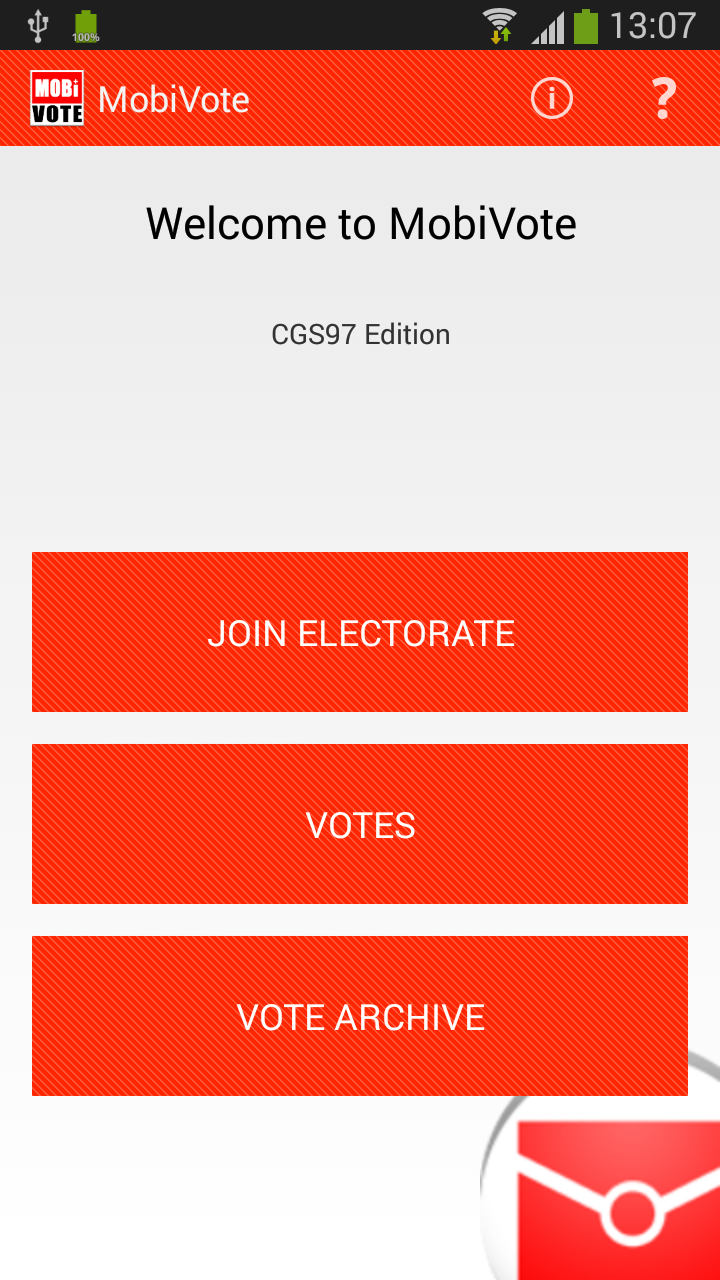
\includegraphics[height=.4\textheight]{img/screenshots/main}
	\caption{MobiVote Main Screen}
	\label{fig:handbook_mainscreen}
\end{figure}

\section{Setup a Vote}
The group needs to nominate one member as the administrator of the vote. The
administrator is responsible for the orchestration of the voting process. That
includes defining the question and the possible options, approving other people
to be in the electorate and initiating the voting phase.

\textbf{Admin only:} In order to setup a new vote, the nominated administrator
selects the option \keys{Votes} on the main screen. The appearing screen shows a list of prepared
votes, as well as an option to create a new vote \myref{fig:handbook_votes}. In
the ``Vote Setup'' screen \myref{fig:handbook_votesetup}, the properties of the
vote can be defined, namely the question of the vote and a list of possible
answers. The option \menu[,]{Allow blank ballots} can be checked if voters
should be allowed to cast a blank ballot.

From here you can either go back if you just want to prepare the vote in advance
for an upcoming session, or you can directly start the vote by clicking on the
button \keys{Start vote}.

\begin{figure}[!htb]
	\begin{minipage}{.5\textwidth}
  		\centering
		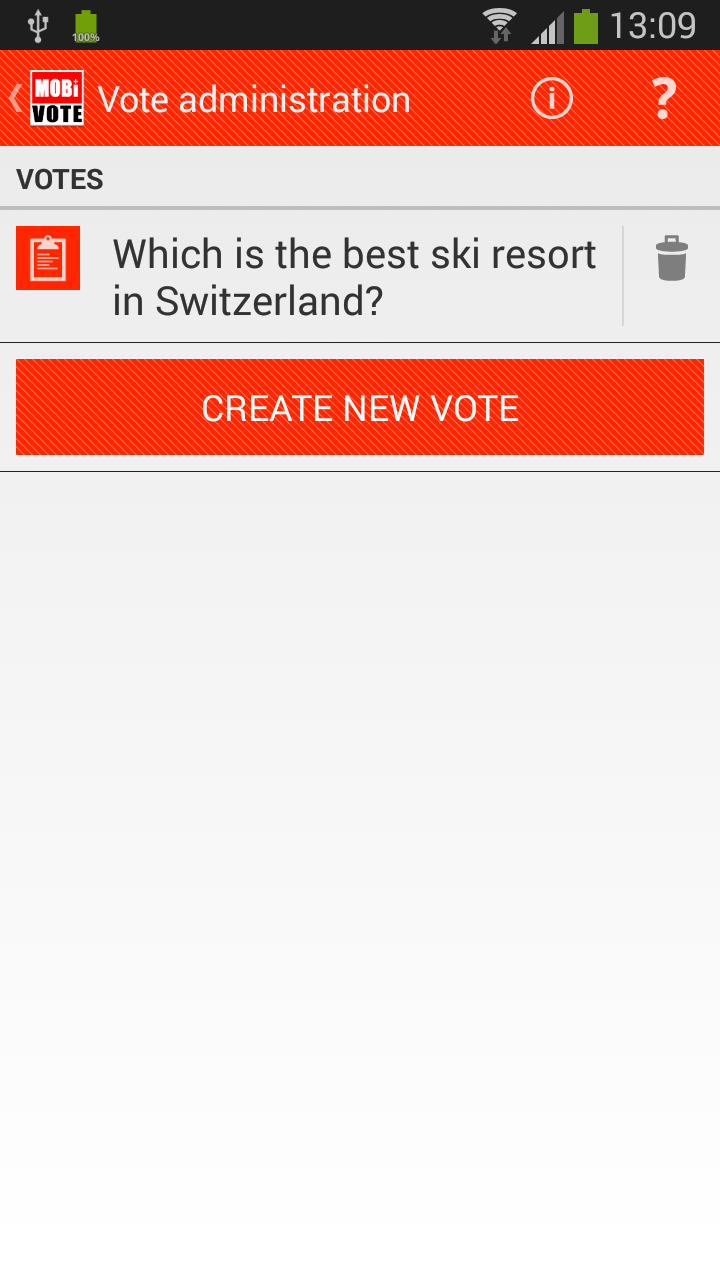
\includegraphics[height=.4\textheight]{img/screenshots/votes}
		\caption{Available Votes}
		\label{fig:handbook_votes}
	\end{minipage}
	\begin{minipage}{.5\textwidth}
  		\centering
		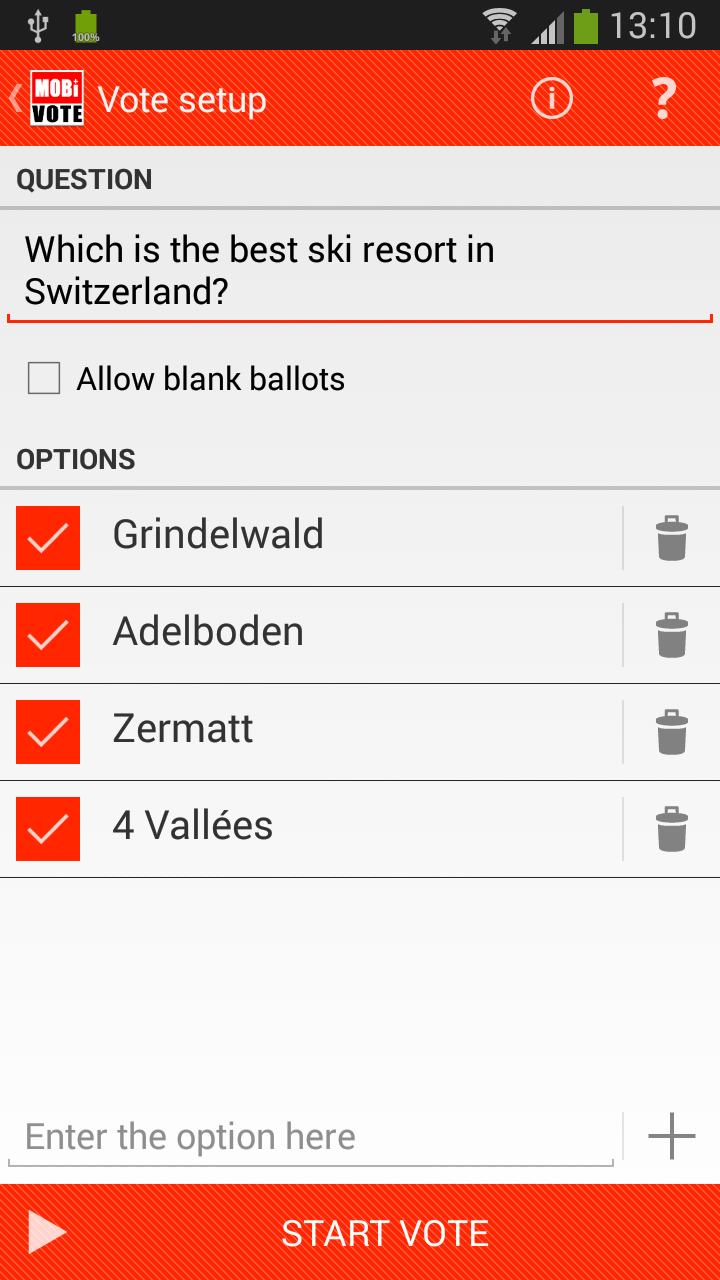
\includegraphics[height=.4\textheight]{img/screenshots/vote_details}
		\caption{Vote Setup}
		\label{fig:handbook_votesetup}
	\end{minipage}
\end{figure}

\section{Start a Voting Session}
\textbf{Admin only:} In order to establish a voting session, some additional
information regarding the network is required. First, you need to enter an identification into the
according textbox at the top of the screen
\myref{fig:handbook_networkconfiguration}. This value defines how you will be
represented in the voting session. Most likely you will want to enter your name
into this box. This value will be saved on the device and will be proposed in
upcoming sessions, but you can change this representation anytime you want to.
Moreover, you are required to tell the application in which wireless network the
voting session should take place. In most cases this will be the network that
you are currently connected to. If you want to use this network, you can just
click on the button \keys{Use network ``XYZ''}. In case you want to use a
different network, you can use the button \keys{Advanced network configuration}.
This screen lets you choose all currently available network
\myref{fig:handbook_advancednetworkconfiguration}. When choosing a network, you
should consider that all the participants need to be allowed to connect to this
network.

\begin{figure}[!htb]
	\begin{minipage}{.5\textwidth}
  		\centering
		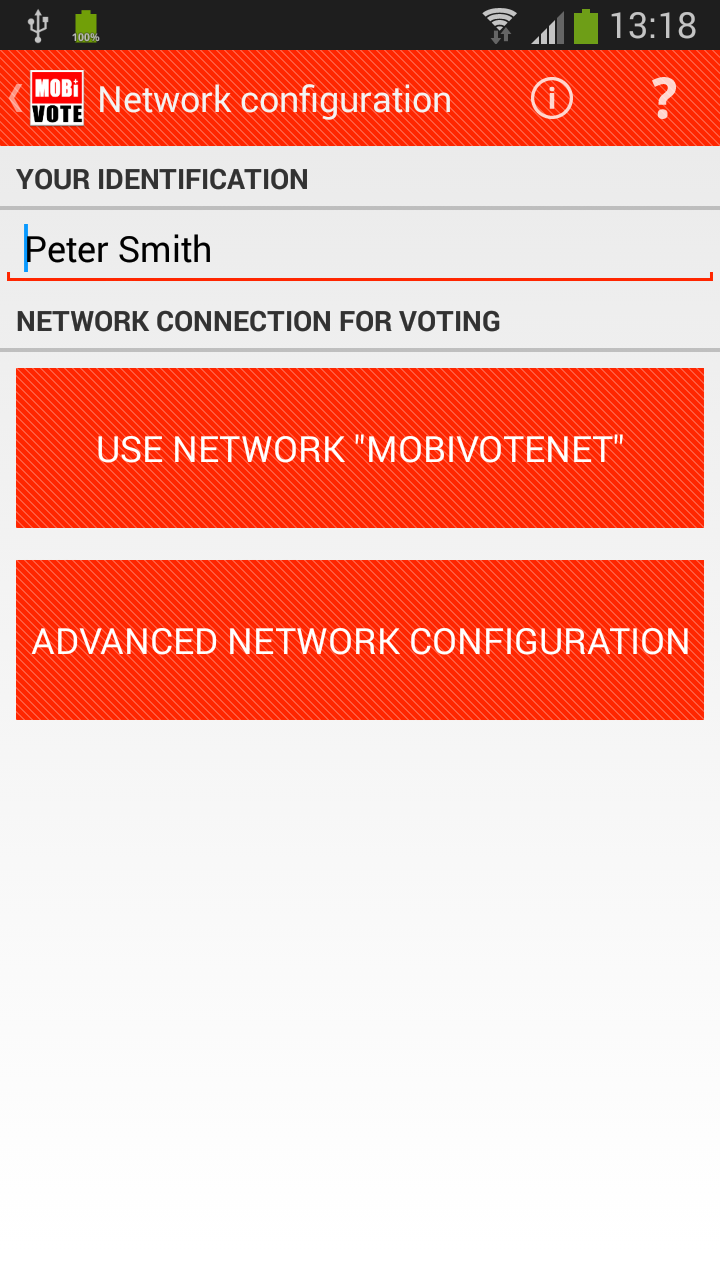
\includegraphics[height=.4\textheight]{img/screenshots/network_configuration}
		\caption{Network Configuration}
		\label{fig:handbook_networkconfiguration}
	\end{minipage}
	\begin{minipage}{.5\textwidth}
  		\centering
		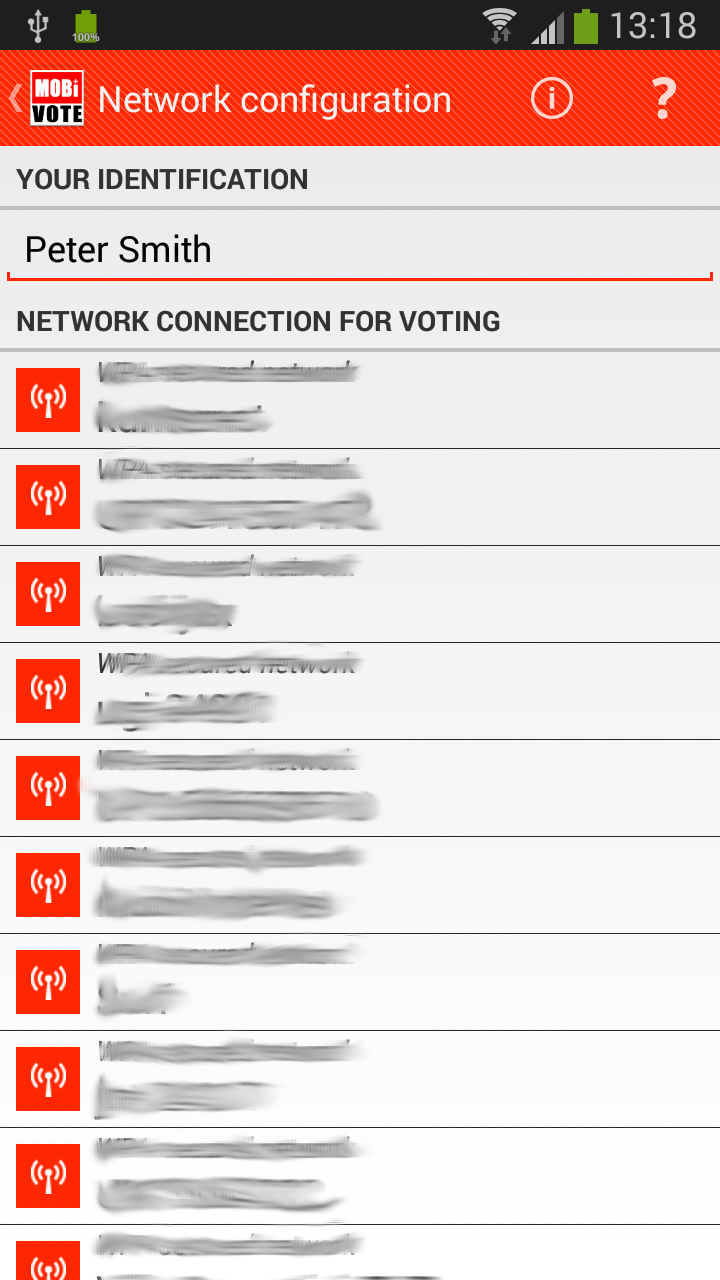
\includegraphics[height=.4\textheight]{img/screenshots/advanced_network_configuration}
		\caption{Advanced Configuration}
		\label{fig:handbook_advancednetworkconfiguration}
	\end{minipage}
\end{figure}

\section{Share the Session Parameters}
After selecting the network, a screen containing the voting session parameters
is displayed \myref{fig:handbook_networkinformation}. Three parameters are
required to connect to a voting session:
\begin{itemize}
  \item The network name (SSID)
  \item The group number
  \item The group password
\end{itemize}

These three parameters need to be distributed to all the persons who will be
allowed to join the electorate of the vote. To do so, MobiVote provides three
ways.
\begin{itemize}
  \item \textbf{Plain text:} All three parameters are communicated visually or
  orally as plain text. The participants can enter them when joining a voting
  session.
  \item \textbf{QR-code:} The three parameters are encoded in a QR-code which is
  displayed on the same screen. This QR-code can then be scanned using the
  camera of the participant's devices.
  \item \textbf{NFC tag:} The three parameters are written to a NFC tag. A NFC
  tag is a small magnetic storage token. An example of a NFC tag is depicted in
  \Vref{fig:handbook_nfctag}. This tag can then be passed along the participants
  who can scan the tag by tapping it to the back of their device. Please note
  that NFC functionality is only available in devices of the latest generation.
\end{itemize}
Of course it is also possible to use a combination of these three options. Using
one of the sharing methods above, the participants can now join the voting
session.

\begin{figure}[!htb]
	\begin{minipage}{.5\textwidth}
  		\centering
		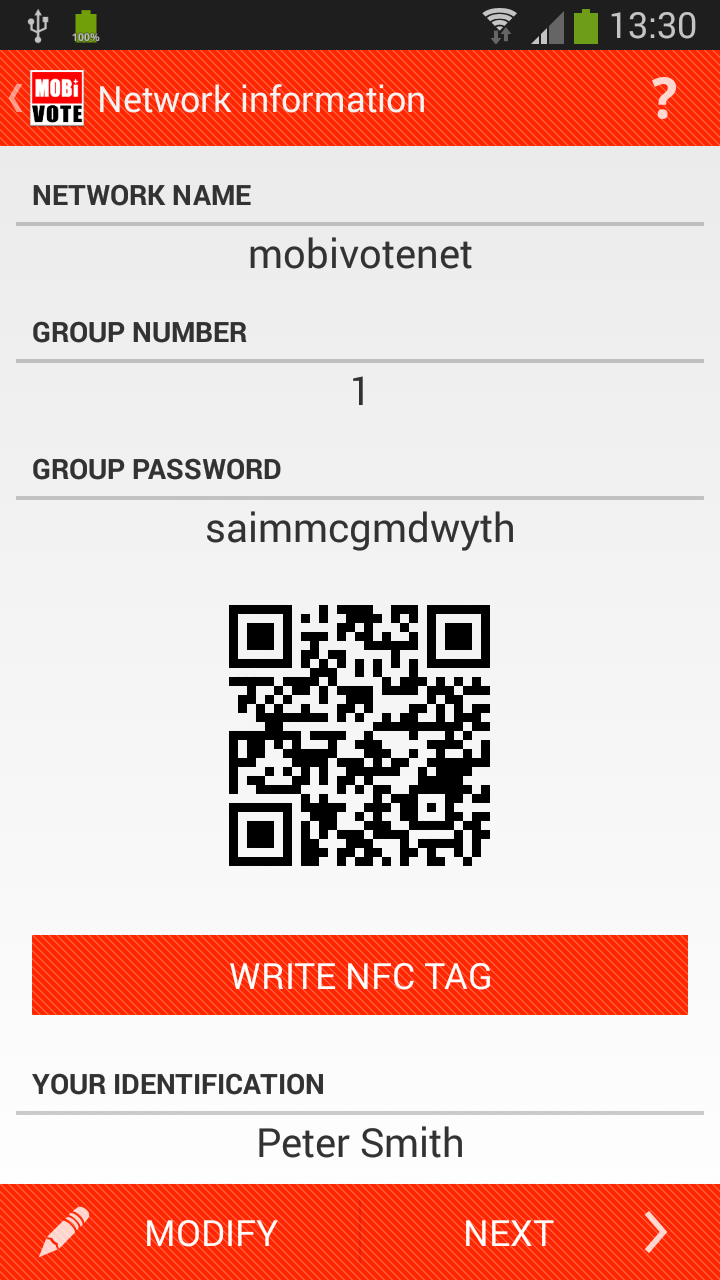
\includegraphics[height=.4\textheight]{img/screenshots/network_information}
		\caption{Network Information}
		\label{fig:handbook_networkinformation}
		\end{minipage}
	\begin{minipage}{.5\textwidth}
  		\centering
		
\includegraphics[height=.2\textheight]{img/nfc_tag}
		\caption{NFC Tag}
		\label{fig:handbook_nfctag}
	\end{minipage}
\end{figure}

\section{Join a Voting Session as a Participant}
\textbf{Voter only:} Once the administrator has announced the session
parameters, the participants can join the session using one of the sharing methods outlined in the previous
section. After starting up the MobiVote app, the participants now chooses the
option \keys{Join electorate}. First, you need to enter an identification into
the according textbox at the top of the screen
\myref{fig:handbook_joinelectorate}. This value defines how you will be
represented in the voting session. Most likely you will want to enter your name
into this box. This value will be saved on the device and will be proposed in
upcoming sessions, but you can change this representation anytime you want to.
Next, one of the following methods to join can be chosen:
\begin{itemize}
  \item \textbf{Scan QR-code:} Using this method, the QR-code displayed on
  another device can be captured using the camera of the device. After the
  successful capture, the device is automatically joined into the voting
  session. In case the session takes place on a secure WLAN which is not known
  on the device, the user will be prompted to enter the WLAN key. This method is
  probably the easiest and fastest way to join a voting session.
  \item \textbf{Use currently connected network:} When choosing this option, the
  WLAN to which the device is currently connected will be used. The user will be
  prompted to enter the password and the group number
  \myref{fig:handbook_joinelectoratepassword}.
  These values are both displayed on the device of the administrator who
  established the voting session.
  \item \textbf{Advanced network configuration:} This option provides you with a
  list of currently available WLAN configuration
  \myref{fig:handbook_advancedconfigurationuser}. In order to join the voting
  session, you need to choose the WLAN which is displayed on the screen of the
  administrator's device. You will then be prompted to enter the password and
  the group number according to the parameters provided by the administrator.
  \item \textbf{Scan NFC tag:} This option can be used if you want to use a NFC
  tag which has been passed to you from the vote administrator
  \myref{fig:handbook_scannfctag}.
  After tapping the NFC tag to the back of the device, the device automatically
  connects to the voting session. In case the session takes place on a secure
  WLAN which is not known on the device, the user will be prompted to enter the
  WLAN key.
  Please note that this option is only available on devices on which NFC
  functionality is available.
\end{itemize}

\begin{figure}[!htb]
	\begin{minipage}{.5\textwidth}
  		\centering
		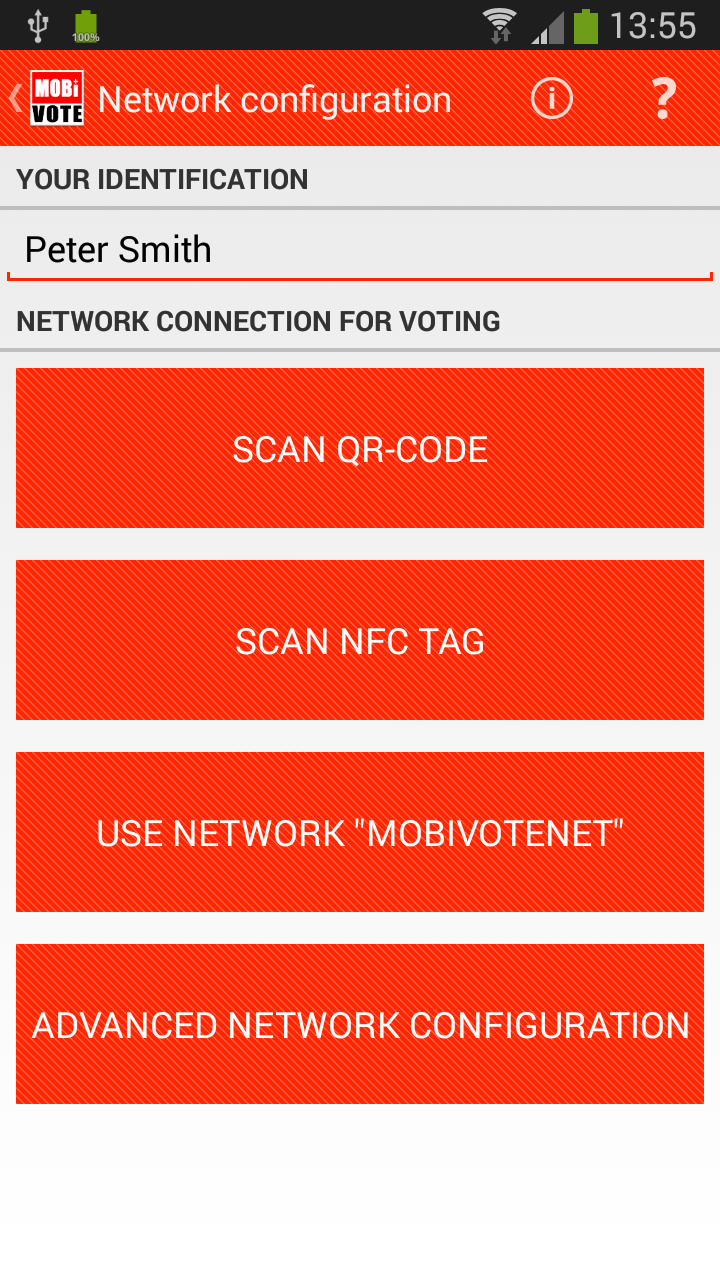
\includegraphics[height=.4\textheight]{img/screenshots/join_electorate}
		\caption{Join Electorate}
		\label{fig:handbook_joinelectorate}
	\end{minipage}
	\begin{minipage}{.5\textwidth}
  		\centering
		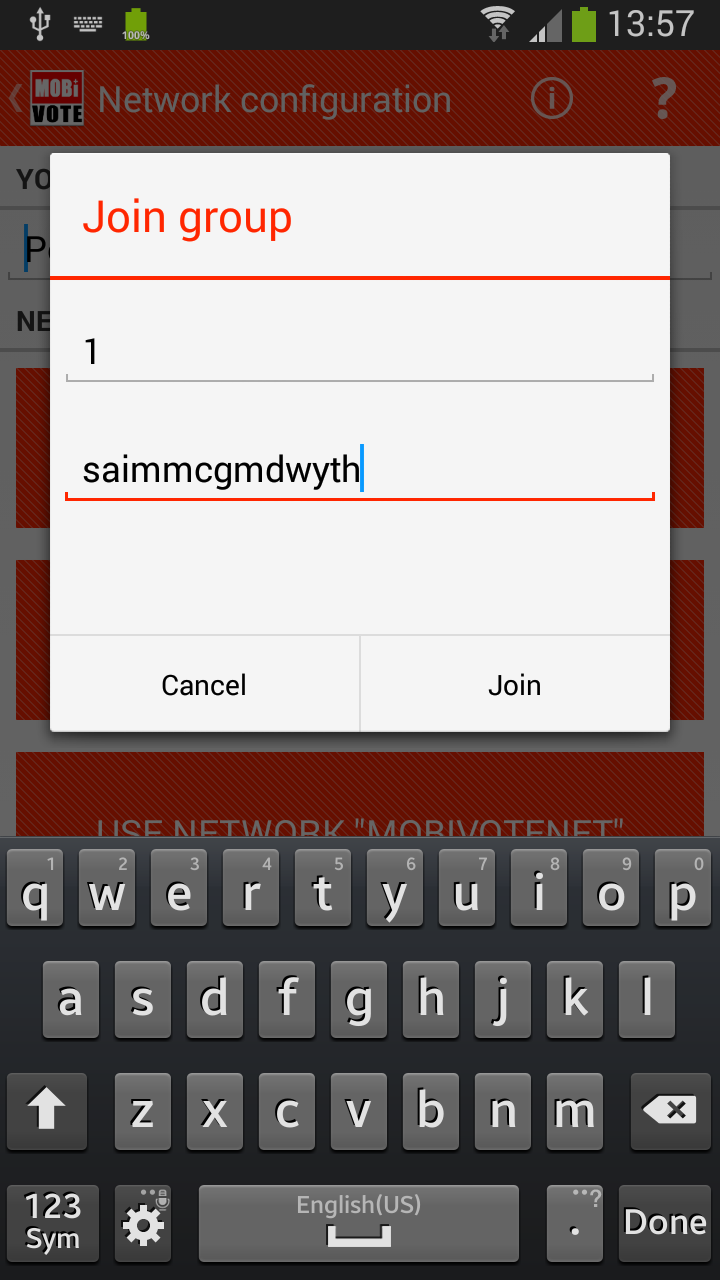
\includegraphics[height=.4\textheight]{img/screenshots/join_electorate_password}
		\caption{Enter Password}
		\label{fig:handbook_joinelectoratepassword}
	\end{minipage}
\end{figure}
\begin{figure}[!htb]
	\begin{minipage}{.5\textwidth}
  		\centering
		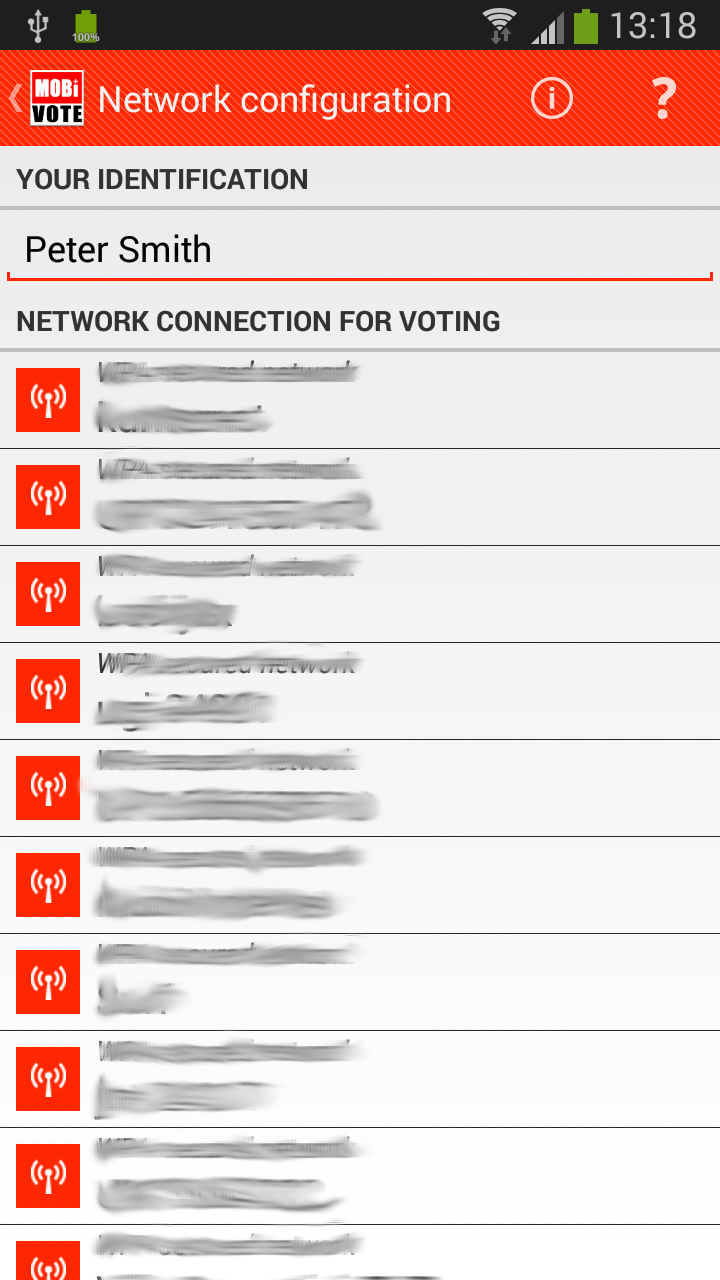
\includegraphics[height=.4\textheight]{img/screenshots/advanced_network_configuration}
		\caption{Advanced Configuration}
		\label{fig:handbook_advancedconfigurationuser}
	\end{minipage}
	\begin{minipage}{.5\textwidth}
  		\centering
		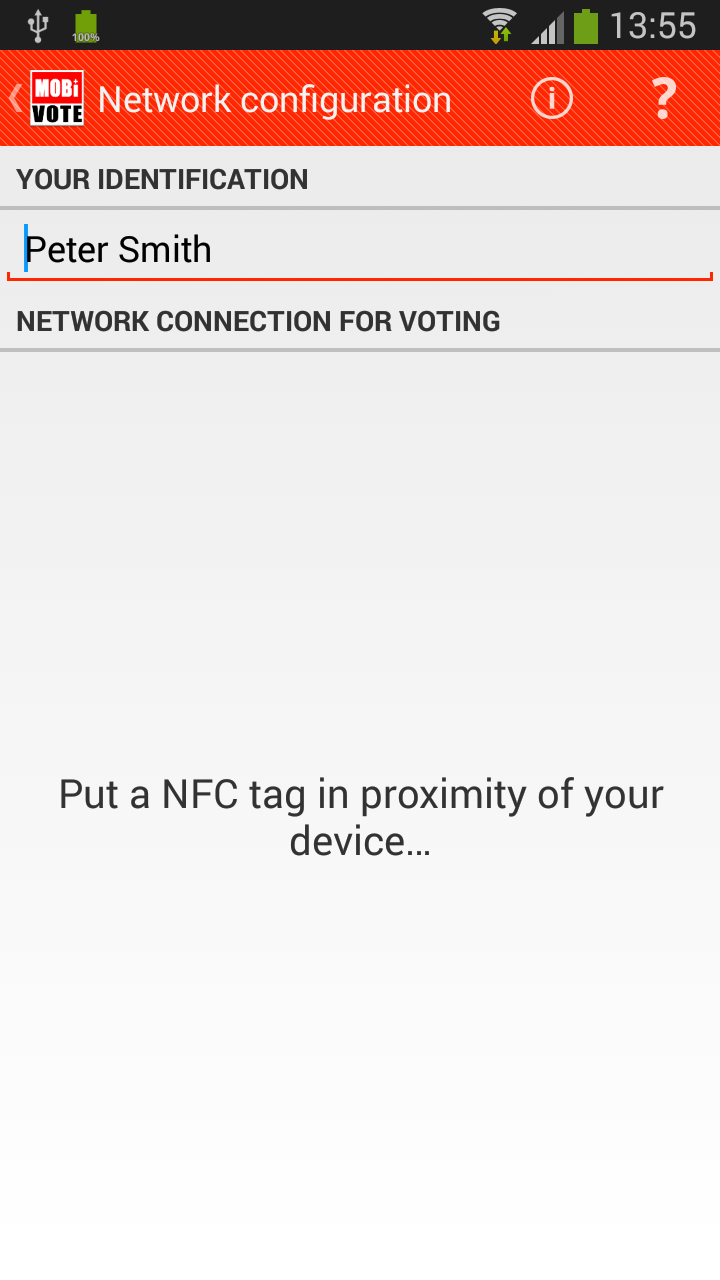
\includegraphics[height=.4\textheight]{img/screenshots/scan_nfc_tag}
		\caption{Scan NFC Tag}
		\label{fig:handbook_scannfctag}
	\end{minipage}
\end{figure}

\section{Define the Electorate}
As soon as all participants were able to join their devices to the voting
session, the administrator can forward to the next screen by clicking on
\keys{Next}. In the following screen \myref{fig:handbook_electorateselection},
the administrator can approve all the joined participants by clicking on the
checkbox next to the allowed participants. Each action reflects
immediately on all the joined devices \myref{fig:handbook_electoratedisplay}.
Please note that the administrator can include or exclude itself in the
electorate.
Furthermore, the administrator has to define a so called \emph{threshold} value.
This value defines how many honest behaving participants need to be available
when the vote is tallied. This value has to lie between two and
the number of participants in the electorate. The value can be adjusted using
the slider at the bottom of the screen.

\begin{figure}[!htb]
	\begin{minipage}{.5\textwidth}
  		\centering
		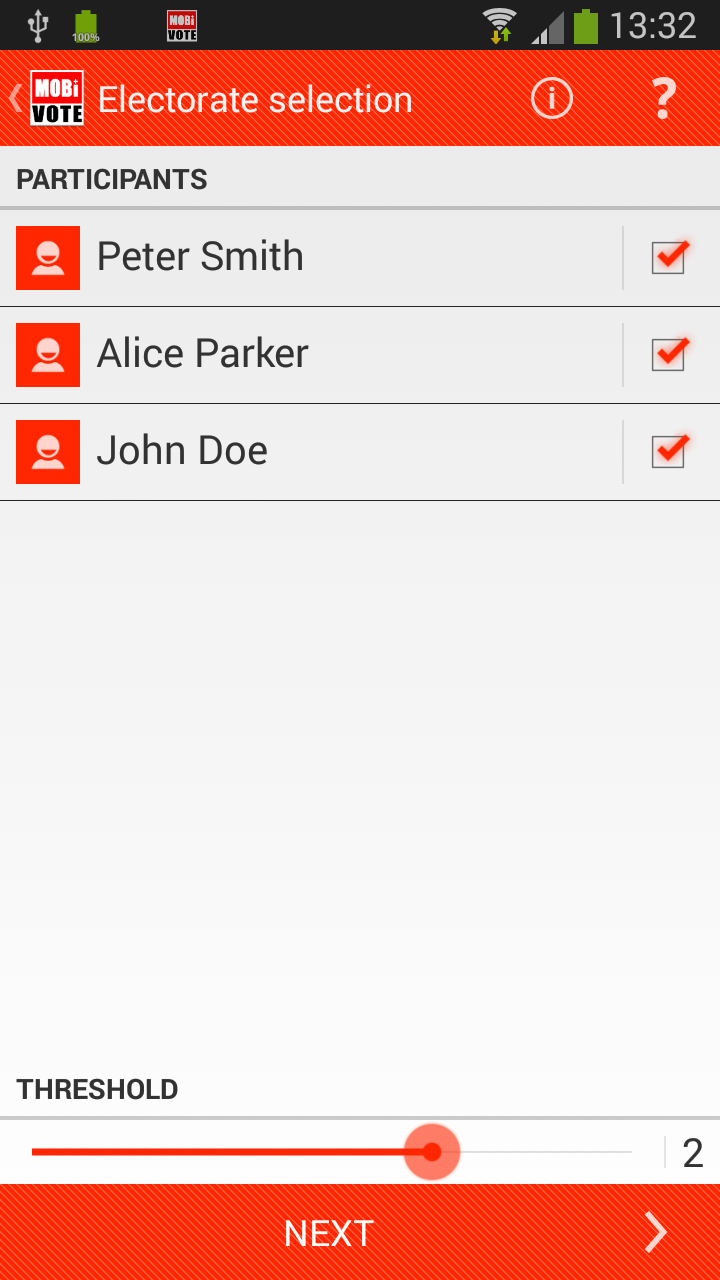
\includegraphics[height=.4\textheight]{img/screenshots/electorate_selection}
		\caption{Admin Defines Electorate}
		\label{fig:handbook_electorateselection}
	\end{minipage}
	\begin{minipage}{.5\textwidth}
  		\centering
		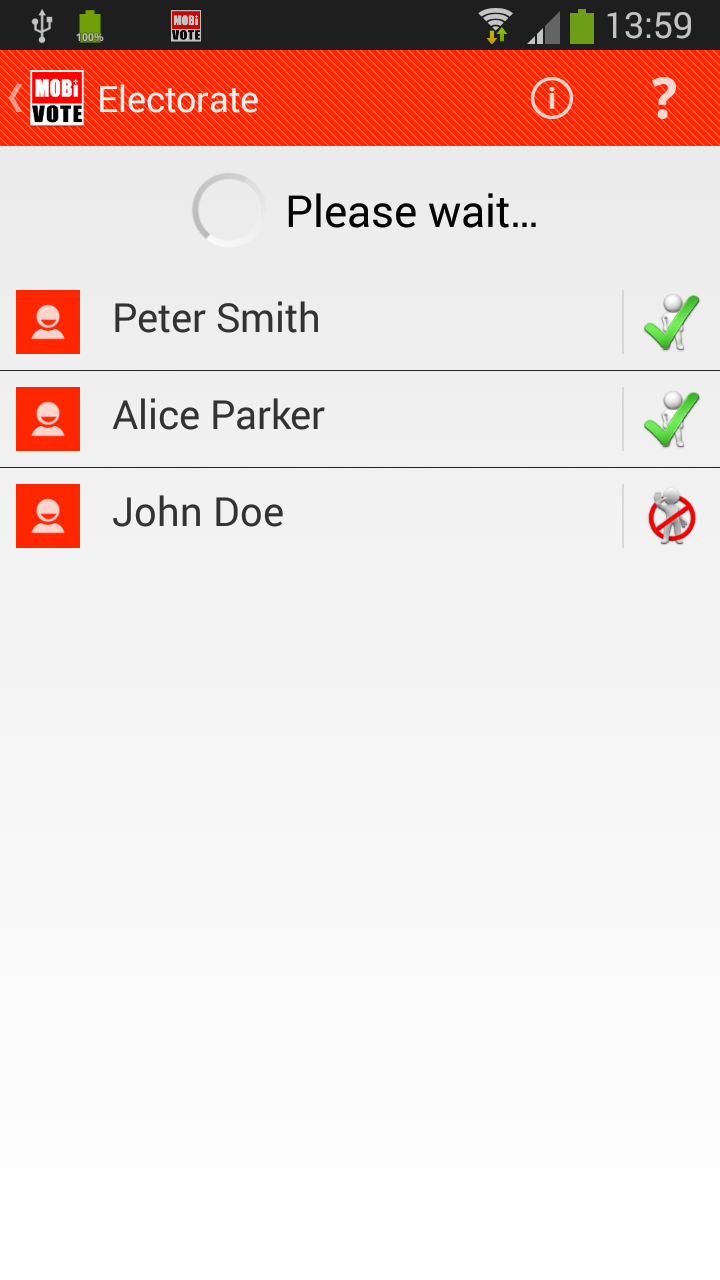
\includegraphics[height=.4\textheight]{img/screenshots/electorate_display}
		\caption{Display Electorate}
		\label{fig:handbook_electoratedisplay}
	\end{minipage}
\end{figure}

\section{Review the Vote}
After having defined the electorate, the administrator can move along the
process by clicking on the \keys{Next} button. This leads to the review screen
\myref{fig:handbook_votereview}, where all the participants see a summary of the
vote and its electorate.
All participants have to agree on this setup by clicking on the checkbox next to
their identification. In case some participants disagree, the administrator can
always go back and adjust the electorate. Once all the participants have agreed
on the setup, the administrator can start the actual voting period by clicking
on the button \keys{Start voting period}.

\begin{figure}[!htb]
	\centering
	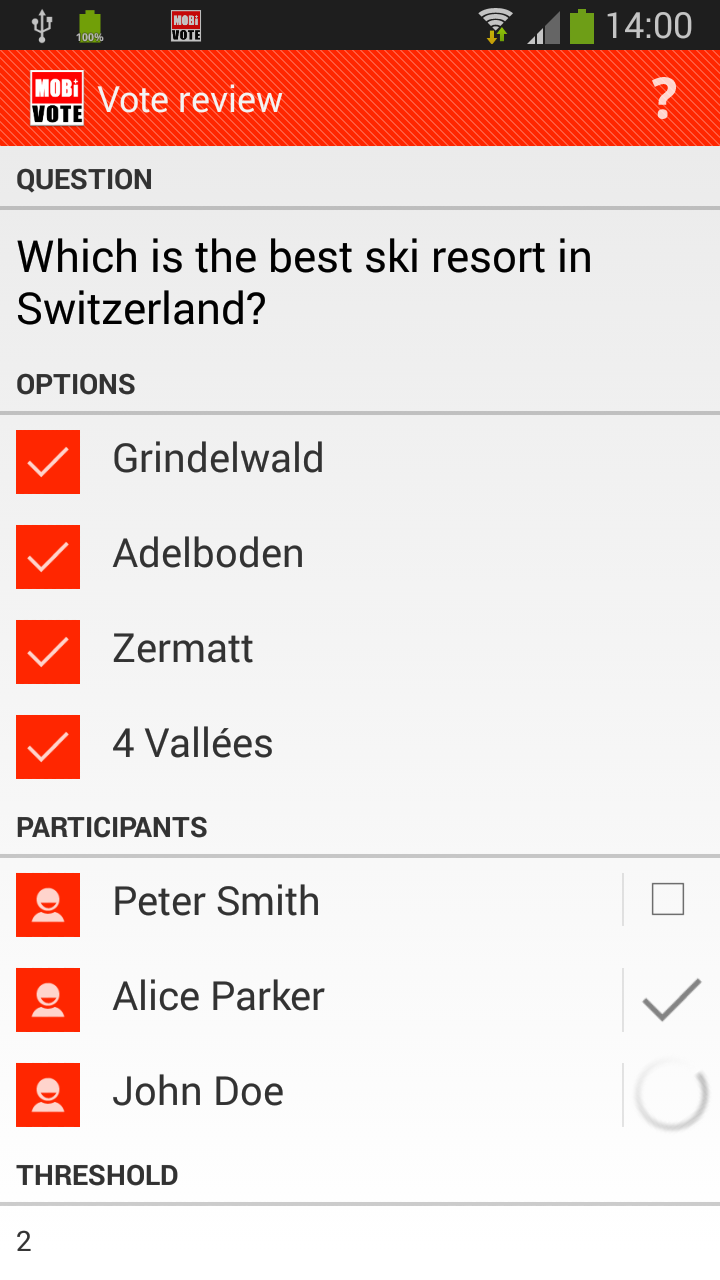
\includegraphics[height=.4\textheight]{img/screenshots/vote_review}
	\caption{Vote Review}
	\label{fig:handbook_votereview}
\end{figure}


\section{Voting}
In the voting screen \myref{fig:handbook_votescreen}, each participant can
select the preferred option.
After confirming the choice, the vote is encrypted and cast. The following
screen \myref{fig:handbook_waitforballots} summarizes which participants cast their votes and which
did not.
The administrator has the option to interrupt by clicking on \keys{Cancel vote}, in
which case no results are obtained. The administrator can also choose the option
\keys{Finish vote}, in which case the vote is tallied and the results are
displayed. The tally of the vote starts automatically as soon as all
participant have cast their votes.

\begin{figure}[!htb]
	\begin{minipage}{.5\textwidth}
  		\centering
		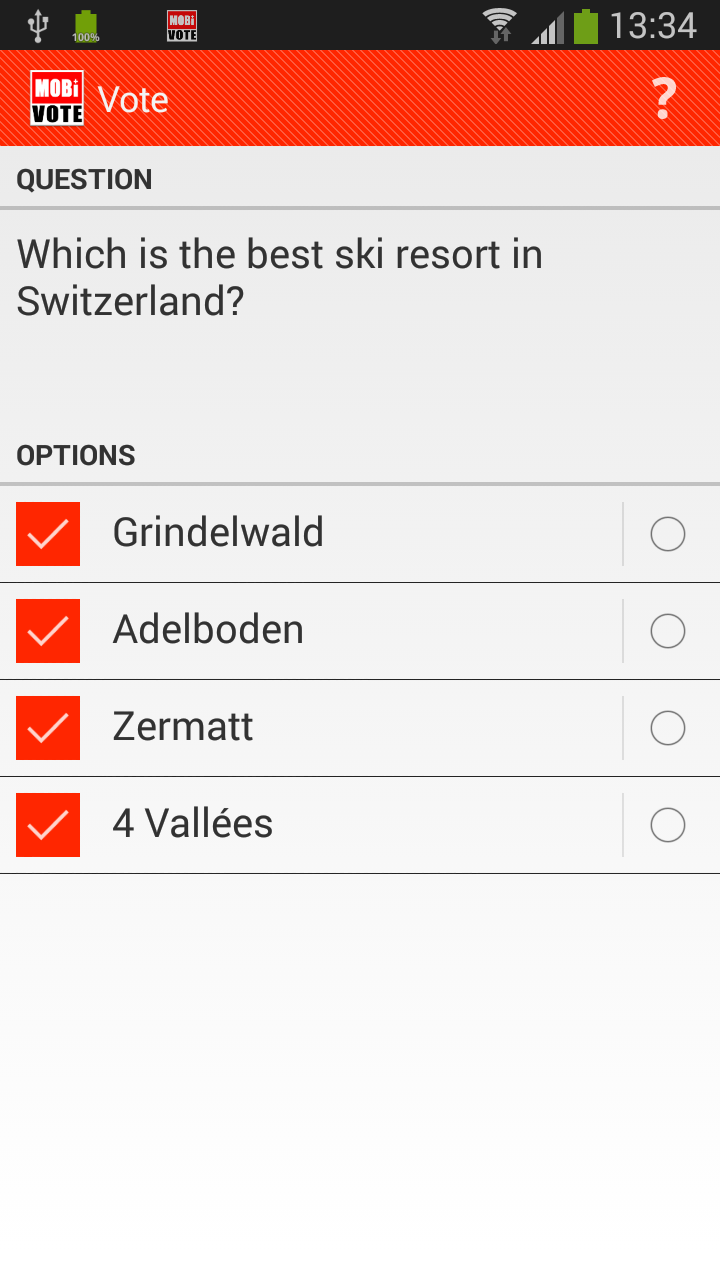
\includegraphics[height=.4\textheight]{img/screenshots/vote}
		\caption{Vote Screen}
		\label{fig:handbook_votescreen}
	\end{minipage}
	\begin{minipage}{.5\textwidth}
  		\centering
		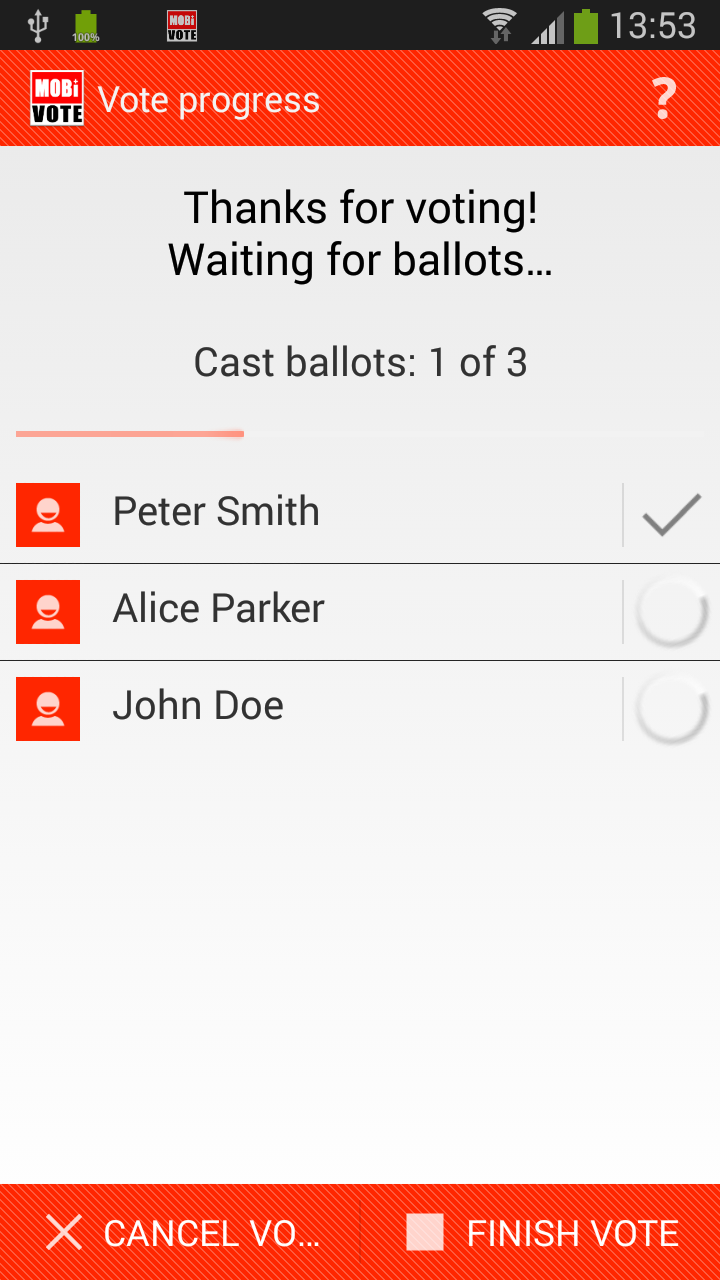
\includegraphics[height=.4\textheight]{img/screenshots/waitforballots}
		\caption{Waiting for Ballots}
		\label{fig:handbook_waitforballots}
	\end{minipage}
\end{figure}

\section{Display the Result}
After a successful tally, you will be redirected to the result screen
\myref{fig:handbook_result} where the result of the vote is displayed along with
some statistics. The vote is archived and can be accessed anytime using the
\keys{Vote archive} option on the main screen. The administrator has the
possibility to repeat the vote. This comes in handy if several voting round are
required to reach a decision.

\begin{figure}[!htb]
	\centering
	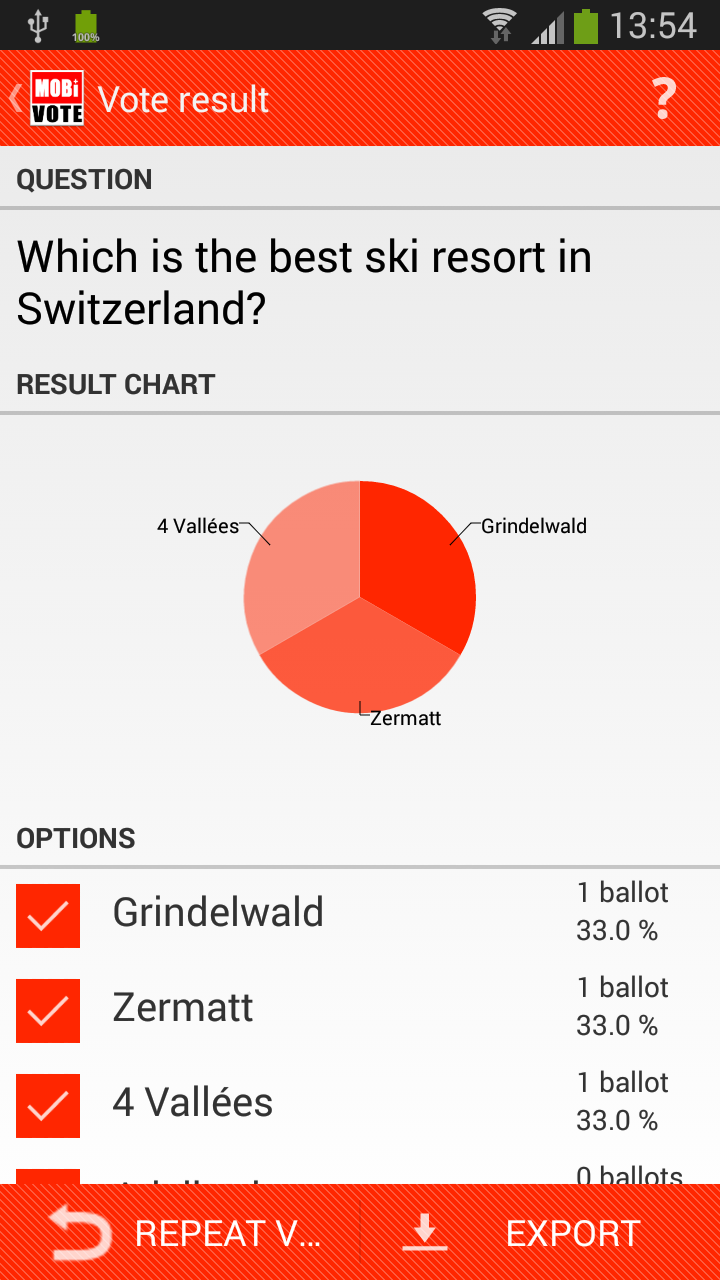
\includegraphics[height=.4\textheight]{img/screenshots/result}
	\caption{Result of the Vote}
	\label{fig:handbook_result}
\end{figure}

\section{Vote Archive}
The vote archive \myref{fig:handbook_votearchive}, which is accessible
through the main screen, lists all the past votes.
Unwanted votes can be deleted using the trash icon on the right side. An
individual vote including the results can be examined in further detail by
clicking on the according list item. If you want to run the exact election
again, the \keys{Clone vote} button can be used to recreate an empty vote which
can then be started in the usual manner. The \keys{Export} button allows to
export the transcript of this vote to an XML file. This file could be used to
verify that the vote has been done correctly. 

\begin{figure}[!htb]
	\centering
	
\includegraphics[height=.4\textheight]{img/screenshots/vote_archive}
	\caption{Vote Archive}
	\label{fig:handbook_votearchive}
\end{figure}

\listoftodos

\end{document}
